%%%%%%%%%%%%%%%%%%%%%%%%%%%%%%%%%%%%%%%%%%%%%%%%%%%%%%%%%%%%%%%%%%%%%%%%%%%%%%%%
\section{Supplementary materials}
%%%%%%%%%%%%%%%%%%%%%%%%%%%%%%%%%%%%%%%%%%%%%%%%%%%%%%%%%%%%%%%%%%%%%%%%%%%%%%%%

These supplementary materials show facets of \verb;pirouette; that did not
fit the main article, such as the installation and an overview of
pirouette's main functions.

Additionally, there is a guide for empicists, based on multiple experiments
that are shown here as well.

For these experiments, we limited the amount of replicates by time, 
aiming at a duration of
24 hours per setting, when run on the computer cluster of the
University of Groningen. Due to this, for example, a run of 40 taxa only
has 6 replicates, as one run takes 4 hours.

All the figures shown in this section are shown as-is, 
without any aesthetical modifications, with the exception that the arrangement
of the sub-figures in subsection \ref{subsec:main_example},
where we aligned parts of the figure by hand.

%%%%%%%%%%%%%%%%%%%%%%%%%%%%%%%%%%%%%%%%%%%%%%%%%%%%%%%%%%%%%%%%%%%%%%%%%%%%%%%%
\subsection{Overview}
%%%%%%%%%%%%%%%%%%%%%%%%%%%%%%%%%%%%%%%%%%%%%%%%%%%%%%%%%%%%%%%%%%%%%%%%%%%%%%%%

\itemize{
  \item{
    subsection \ref{subsec:guidelines}: guidelines for empiricists
  }
  \item{
    subsection \ref{subsec:installation}: installation
  }
  \item{
    subsection \ref{subsec:resources}: resources, such as 
    website, tutorials, packages used, bug reporting and contributing
  }
  \item{
    subsection \ref{subsec:citation}: citation of pirouette
  }
  \item{
    subsection \ref{subsec:main_functions}: main functions
  }
  \item{
    subsection \ref{subsec:main_example}: extra figures and
    diagnostics regarding the main example.
  }
  \item{
    subsection \ref{subsec:distribution}: the result of using 
    multiple trees, as generated by the
    same stochastic process as the main example
  }
  \item{
    subsection \ref{subsec:n_taxa}: the effect of the number
    of taxa
  }
  \item{
    subsection \ref{subsec:n_nucleotides}: the effect of the DNA
    alignment sequence length
  }
  \item{
    subsection \ref{subsec:non_clock}: the effect when the alignment
    is generated by a non-clock like nucleotide substitution model
  }
  \item{
    subsection \ref{subsec:simplest_correct_parameterization} shows the
    effect when doing an inference in the simplest use case
  }
  \item{
    subsection \ref{subsec:under_parameterization} shows the
    effect when doing an inference with an under-parameterization
  }
  \item{
    subsection \ref{subsec:different_n_mutations} shows the
    effect when the twin alignment is allowed to have a different
    number of mutations
  }
  \item{
    subsection \ref{subsec:mutation_rate} shows the
    effect of different mutation rates
  }
}

%%%%%%%%%%%%%%%%%%%%%%%%%%%%%%%%%%%%%%%%%%%%%%%%%%%%%%%%%%%%%%%%%%%%%%%%%%%%%%%%
\subsection{Guidelines for empiricists}
\label{subsec:guidelines}
%%%%%%%%%%%%%%%%%%%%%%%%%%%%%%%%%%%%%%%%%%%%%%%%%%%%%%%%%%%%%%%%%%%%%%%%%%%%%%%%

From the experiments shown below, we composed some rough guidelines.
These guidelines should be treated as preliminary results, as
the total runtime of these experiments is 'only' 19 days.

\itemize{
  \item the use of 20 replicates results in decent plots
  \item the use of more taxa, counterintuitively, increases the inference error
  \item the use of longer DNA sequences, as expected, decreases the inference error
  \item {
    there is a difference when a twin alignment is selected to have
    an equal amount of mutations as the true alignment. The consequences
    of this is unknown
  }
  \item {
    using a mutation rate less than 1.0 / crown age, decreases the
    inference error. We predict this will increase the error in the parameter
    estimation
  }
}

%%%%%%%%%%%%%%%%%%%%%%%%%%%%%%%%%%%%%%%%%%%%%%%%%%%%%%%%%%%%%%%%%%%%%%%%%%%%%%%%
\subsection{Installation}
\label{subsec:installation}
%%%%%%%%%%%%%%%%%%%%%%%%%%%%%%%%%%%%%%%%%%%%%%%%%%%%%%%%%%%%%%%%%%%%%%%%%%%%%%%%

\verb;pirouette; will be made available on CRAN from which 
it can then be easily installed:
\begin{lstlisting}[language=R, floatplacement=ht, frame=single]
install.packages("pirouette")
\end{lstlisting}

Until it is on CRAN, and for the most up-to-date version, 
one can download and install the package from \verb;pirouette;'s GitHub 
repository:

\begin{lstlisting}[
    language = R,
    floatplacement = ht,
    frame = single
]
remotes::install_github(
  "richelbilderbeek/pirouette"
)
\end{lstlisting}
To start using \verb;pirouette;, 
load its functions in the global namespace first:
\begin{lstlisting}[language=R, floatplacement=ht, frame=single]
library(pirouette)
\end{lstlisting}
Because \verb;pirouette; calls BEAST2, BEAST2 must be installed. 
This can be done from within R, using:
\begin{lstlisting}[language=R, floatplacement=ht, frame=single]
install_beast2()
\end{lstlisting}
For the option to select the best candidate model,
\verb;pirouette; needs the "NS" BEAST2 package [\cite{russel2019model}].
It can be installed from within R, using:
\begin{lstlisting}[language=R, floatplacement=ht, frame=single]
install_beast2_pkg("NS")
\end{lstlisting}

%%%%%%%%%%%%%%%%%%%%%%%%%%%%%%%%%%%%%%%%%%%%%%%%%%%%%%%%%%%%%%%%%%%%%%%%%%%%%%%%
\section{Resources}
\label{subsec:resources}
%%%%%%%%%%%%%%%%%%%%%%%%%%%%%%%%%%%%%%%%%%%%%%%%%%%%%%%%%%%%%%%%%%%%%%%%%%%%%%%%

\verb;pirouette; is free, libre and open source software available at 
\url{http://github.com/richelbilderbeek/pirouette},
licensed under the GNU General Public License version 3.
\verb;pirouette; depends on multiple packages, which are:
\verb;ape; [\cite{ape}],
\verb;assertive; [\cite{assertive}],
\verb;babette; [\cite{bilderbeek2018babette}],
\verb;DDD; [\cite{DDD}],
\verb;devtools; [\cite{devtools}],
\verb;dplyr; [\cite{dplyr}],
\verb;ggplot2; [\cite{ggplot2}],
\verb;knitr; [\cite{knitr}],
\verb;lintr; [\cite{lintr}],
\verb;magrittr; [\cite{magrittr}],
\verb;mcbette; [\cite{mcbette}],
\verb;nLTT; [\cite{nLTT}],
\verb;phangorn; [\cite{phangorn}],
\verb;phytools; [\cite{phytools}],
\verb;plyr; [\cite{plyr}],
\verb;rappdirs; [\cite{rappdirs}],
\verb;rmarkdown; [\cite{rmarkdown}],
\verb;Rmpfr; [\cite{Rmpfr}],
\verb;stringr; [\cite{stringr}],
\verb;TESS; [\cite{TESS}],
\verb;testit; [\cite{testit}], 
\verb;testthat; [\cite{testthat}] and
\verb;tidyr; [\cite{tidyr}].

\verb;pirouette;'s development takes place on GitHub,
\url{https://github.com/richelbilderbeek/pirouette},
which allows submitting bug reports, requesting features, 
and adding code. To ensure a high quality, \verb;pirouette; 
uses a continuous integration service, has a code coverage of above 95\%
and enforces the most commonly used R style guide [\cite{style_guide}].

\verb;pirouette;'s is extensively documented on its website,
its documentation and its vignettes.
The \verb;pirouette; website is a good starting point to learn
how to use \verb;pirouette;, as it links to tutorials and videos.
The \verb;pirouette; package documentation describes
all functions and liberally links to related functions.
All exported functions show a minimal example as part of their documentation.
The \verb;pirouette; vignette demonstrates extensively how 
to use \verb;pirouette; in a more informally written way. 

The code used in this article and more examples that are periodically 
tested, can be found at 
\url{https://github.com/richelbilderbeek/pirouette_examples}. 

%%%%%%%%%%%%%%%%%%%%%%%%%%%%%%%%%%%%%%%%%%%%%%%%%%%%%%%%%%%%%%%%%%%%%%%%%%%%%%%%
\subsection{Citation of pirouette}
\label{subsec:citation}
%%%%%%%%%%%%%%%%%%%%%%%%%%%%%%%%%%%%%%%%%%%%%%%%%%%%%%%%%%%%%%%%%%%%%%%%%%%%%%%%

To cite \verb;pirouette; this article from within R, use:

\begin{lstlisting}[language=R]
> citation("pirouette")
\end{lstlisting}

%%%%%%%%%%%%%%%%%%%%%%%%%%%%%%%%%%%%%%%%%%%%%%%%%%%%%%%%%%%%%%%%%%%%%%%%%%%%%%%%
\subsection{Main functions}
\label{subsec:main_functions}
%%%%%%%%%%%%%%%%%%%%%%%%%%%%%%%%%%%%%%%%%%%%%%%%%%%%%%%%%%%%%%%%%%%%%%%%%%%%%%%%

An overview of \verb;pirouette;'s main functions is shown in 
Table~\ref{tab:functions}. 
All \verb;pirouette;'s functions are documented,
have a useful example and sensible defaults.

%%%%%%%%%%%%%%%%%%%%%%%%%%%%%%%%%%%%%%%%%%%%%%%%%%%%%%%%%%%%%%%%%%%%%%%%%%%%%%%%
\begin{table}[h]
  \centering
  \begin{tabular}{ | l | l | l | }
    \hline
    \textbf{Name} & \textbf{Description} \\
    \hline
    \verb;pir_run; & Run \verb;pirouette; \\
    \verb;pir_plot; & Show the \verb;pirouette; results as a plot  \\
    \verb;create_pir_params; & Create the \verb;pirouette; parameters  \\
    \hline
    \verb;create_alignment_params; & Create the alignment parameters  \\
    \verb;create_twinning_params; & Create the twinning parameters  \\
    \verb;create_experiment; & Create one experiment  \\
    \verb;create_error_measure_params; & Create the error measurement parameters  \\
    \hline
  \end{tabular}
  \caption{
    \texttt{pirouette}'s main functions and description. 
  }
  \label{tab:functions}
\end{table}
%%%%%%%%%%%%%%%%%%%%%%%%%%%%%%%%%%%%%%%%%%%%%%%%%%%%%%%%%%%%%%%%%%%%%%%%%%%%%%%%

%%%%%%%%%%%%%%%%%%%%%%%%%%%%%%%%%%%%%%%%%%%%%%%%%%%%%%%%%%%%%%%%%%%%%%%%%%%%%%%%
\subsection{Main example}
\label{subsec:main_example}
%%%%%%%%%%%%%%%%%%%%%%%%%%%%%%%%%%%%%%%%%%%%%%%%%%%%%%%%%%%%%%%%%%%%%%%%%%%%%%%%

This subsection shows the diagnostics from the main example, which
uses one tree.

The code used in this part of the article can be found at 
\url{https://github.com/richelbilderbeek/pirouette_example_30}.

%%%%%%%%%%%%%%%%%%%%%%%%%%%%%%%%%%%%%%%%%%%%%%%%%%%%%%%%%%%%%%%%%%%%%%%%%%%%%%%%
\begin{figure}[H]
  \centering
  \resizebox {1.0\columnwidth} {!} {
    \begin{tikzpicture}[
      ->,>=stealth',shorten >=1pt,auto,
      node distance=0.5\textheight, 
      semithick
    ]   
    \tikzstyle{every state}=[]
    \node[state, draw=none] (O) [] {
    };   
    \node[state] (A) [right of = O, rectangle] {
      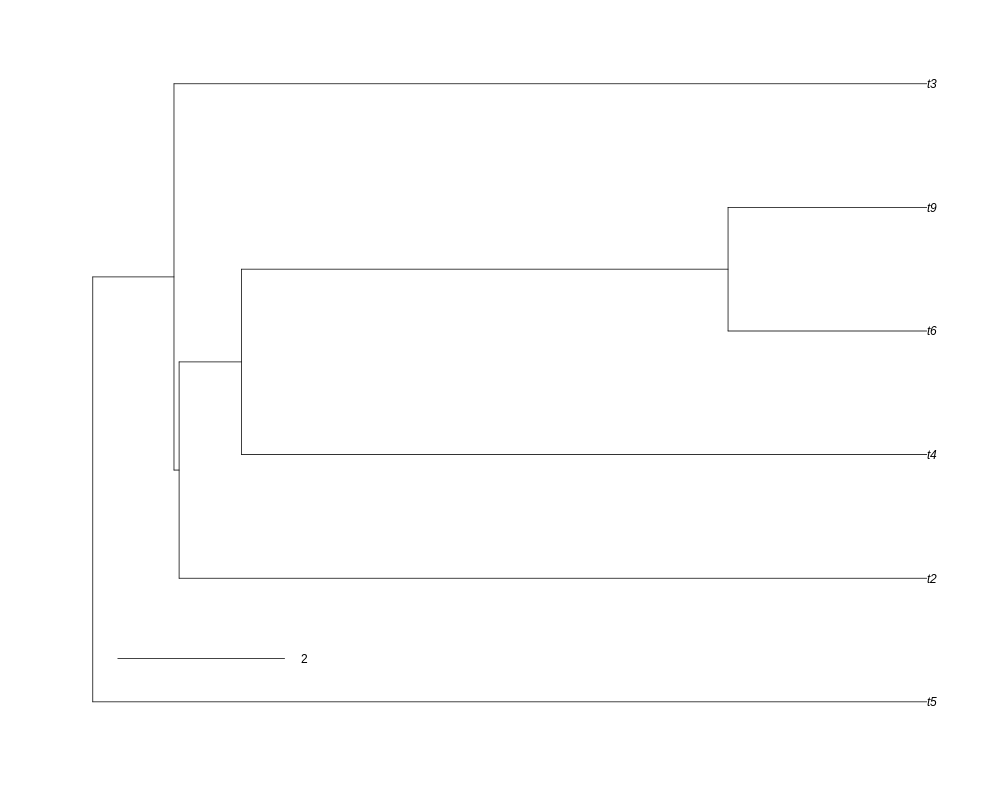
\includegraphics[height=0.4\textheight]{pirouette_example_30/example_30_314/true_tree.png}
    };   
    \node[state] (B) [below of = A, rectangle] {
      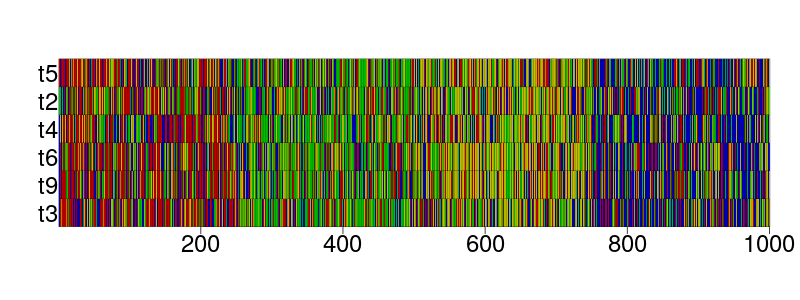
\includegraphics[height=0.25\textheight]{pirouette_example_30/example_30_314/true_alignment.png}
    };   
    \node[state] (CG) [below of = B, rectangle] {
      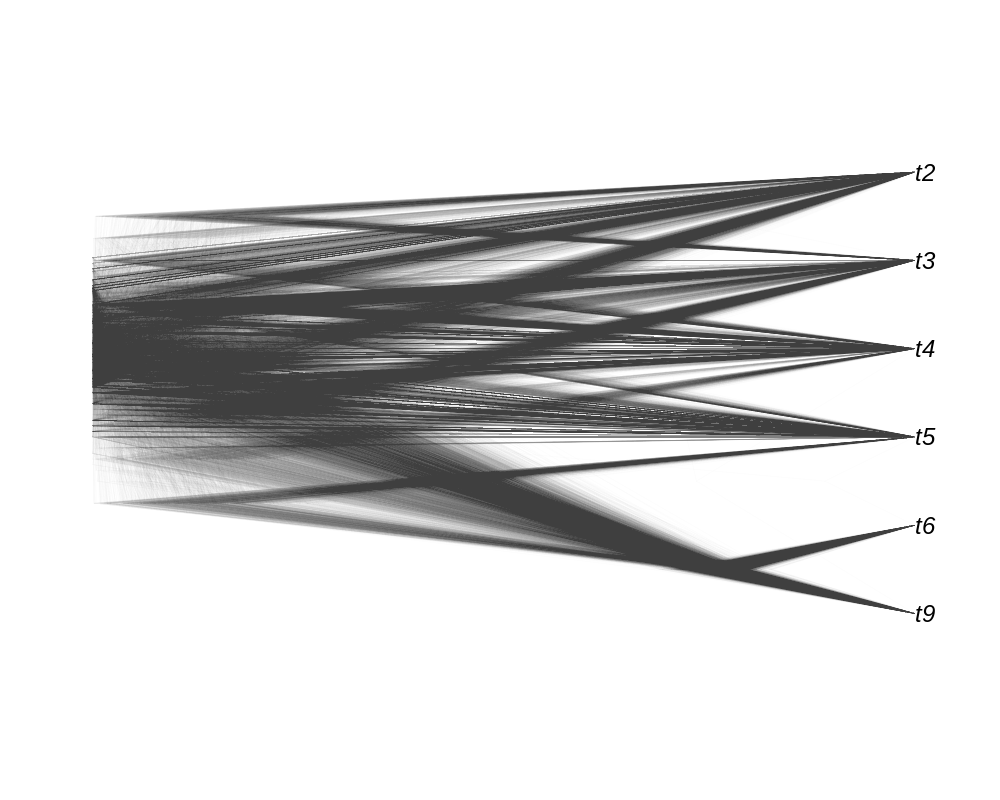
\includegraphics[height=0.3\textheight]{pirouette_example_30/example_30_314/true_posterior_gen.png}
    };   
    \node[state] (DG) [below of = CG, rectangle] {
      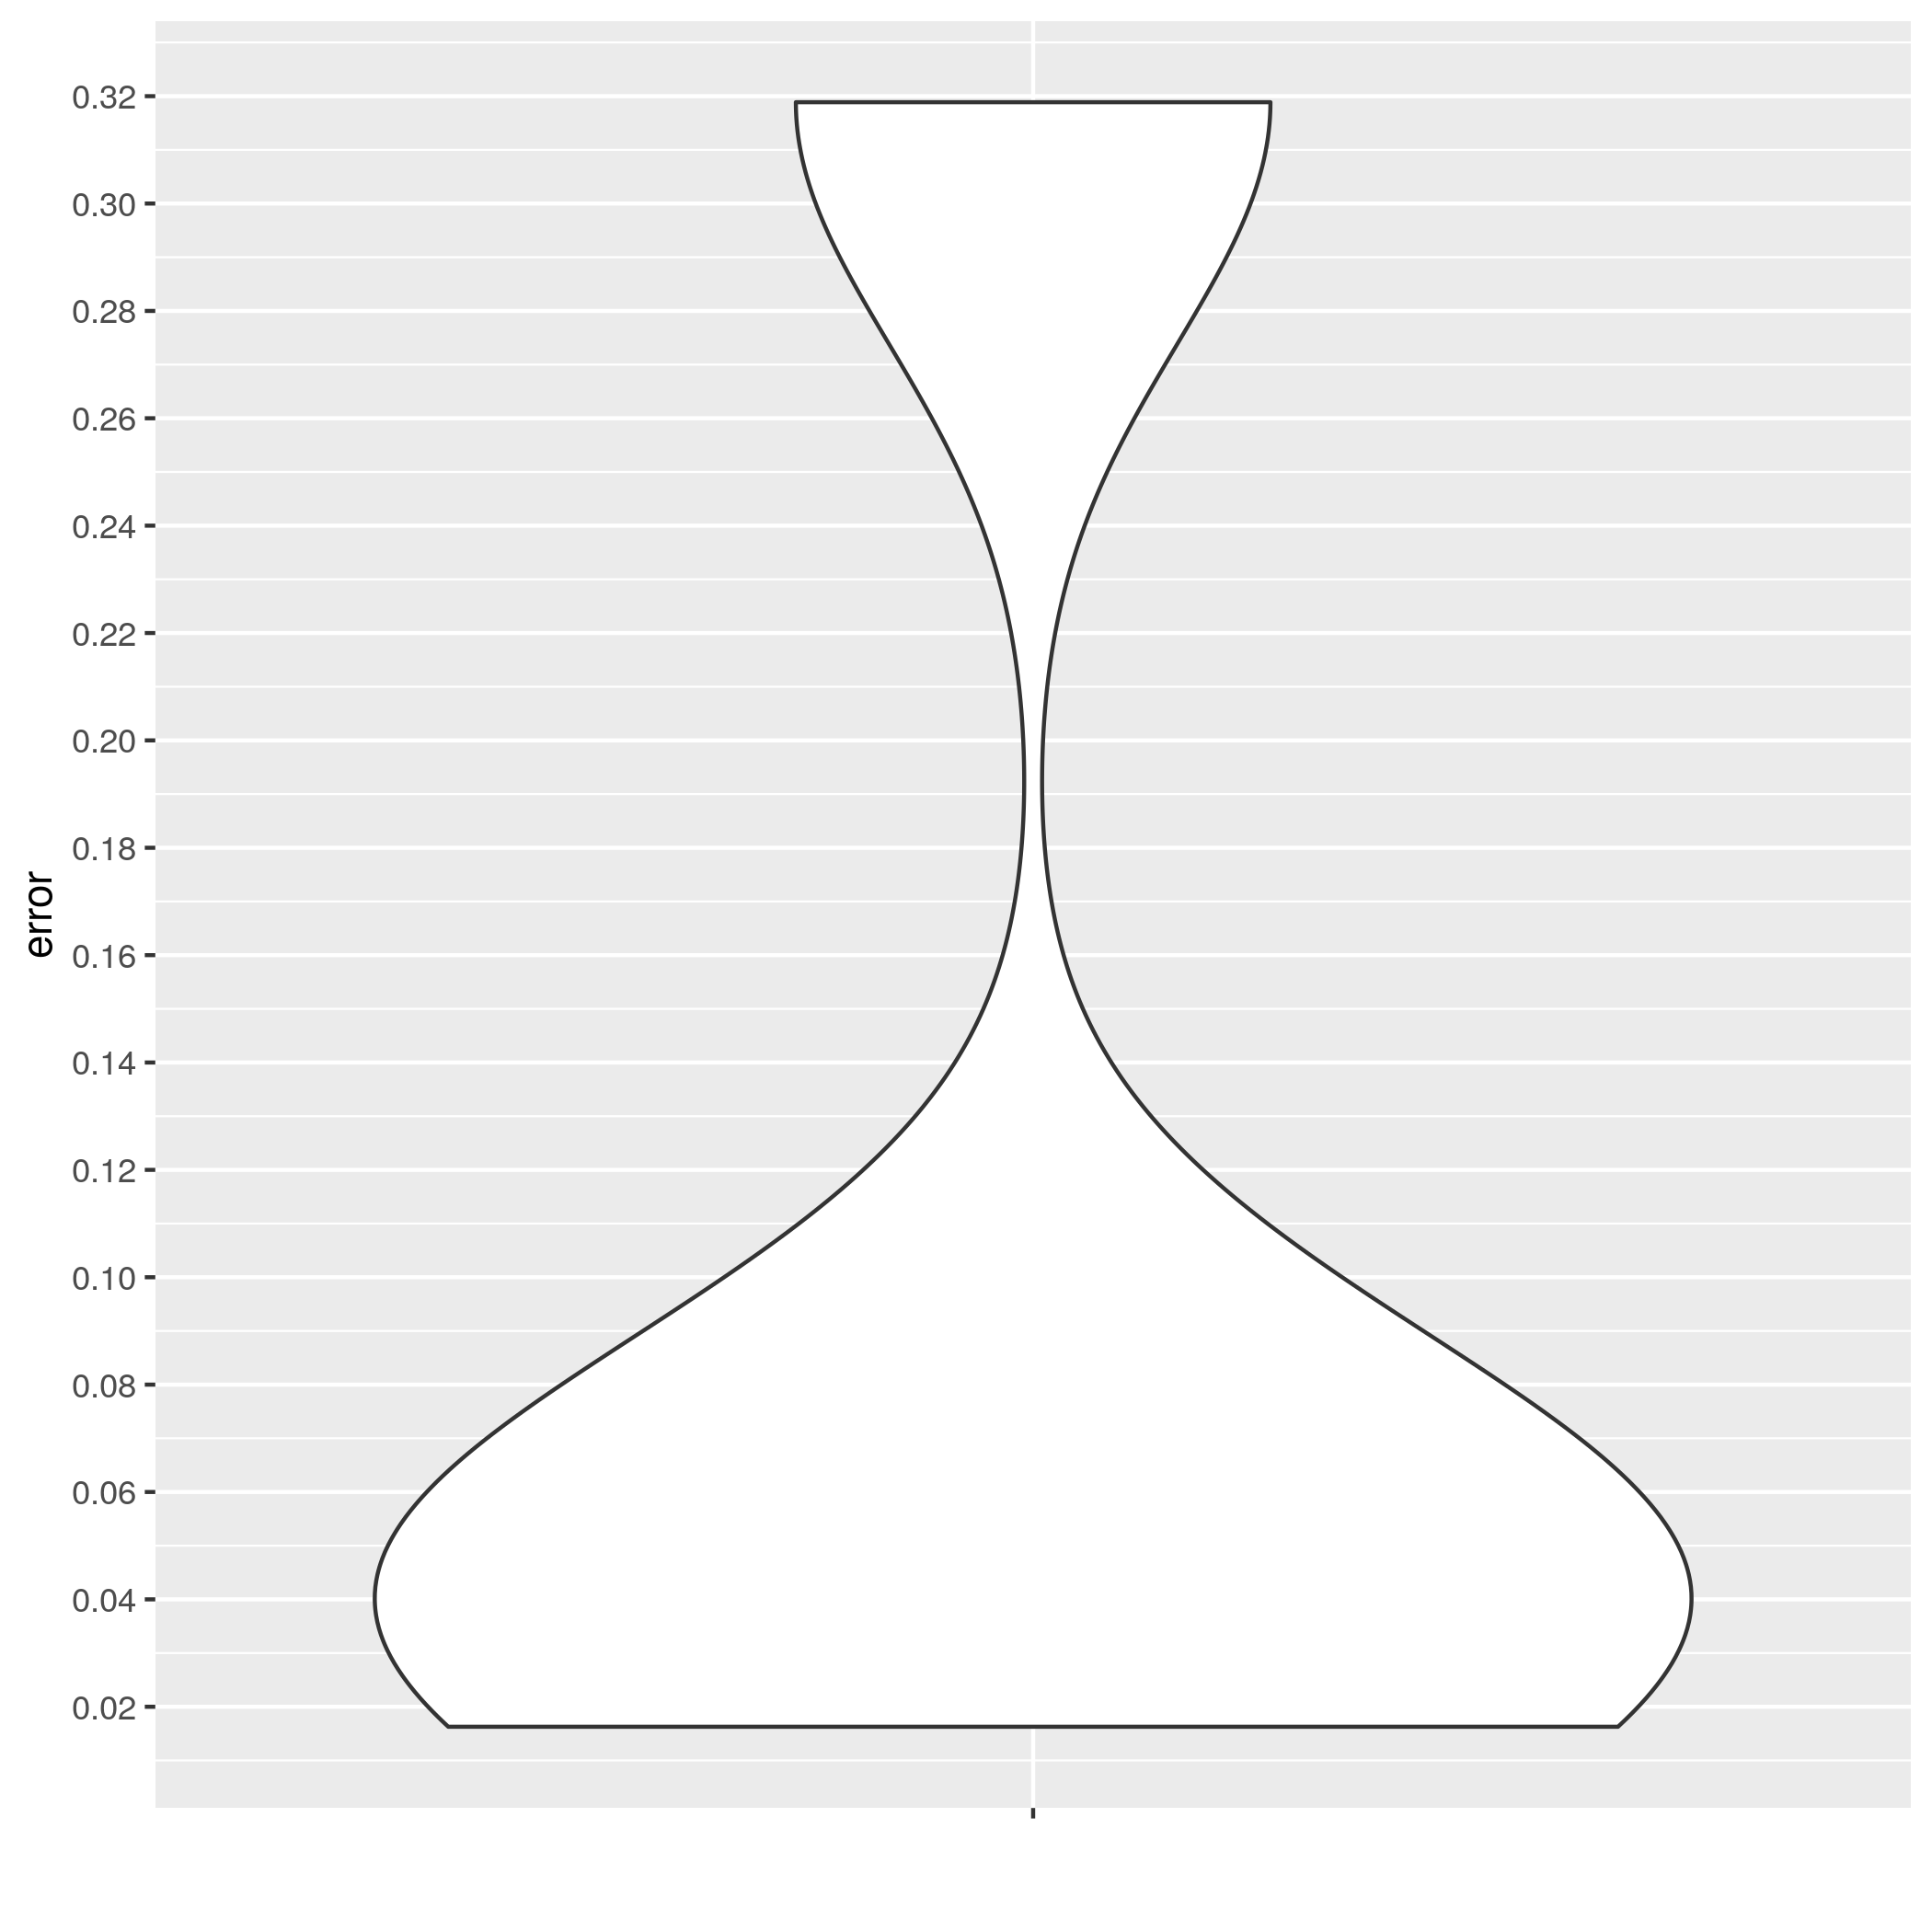
\includegraphics[height=0.3\textheight]{pirouette_example_30/example_30_314/true_error_violin_gen.png}
    };   
    \node[state] (CB) [right of = CG, rectangle] {
      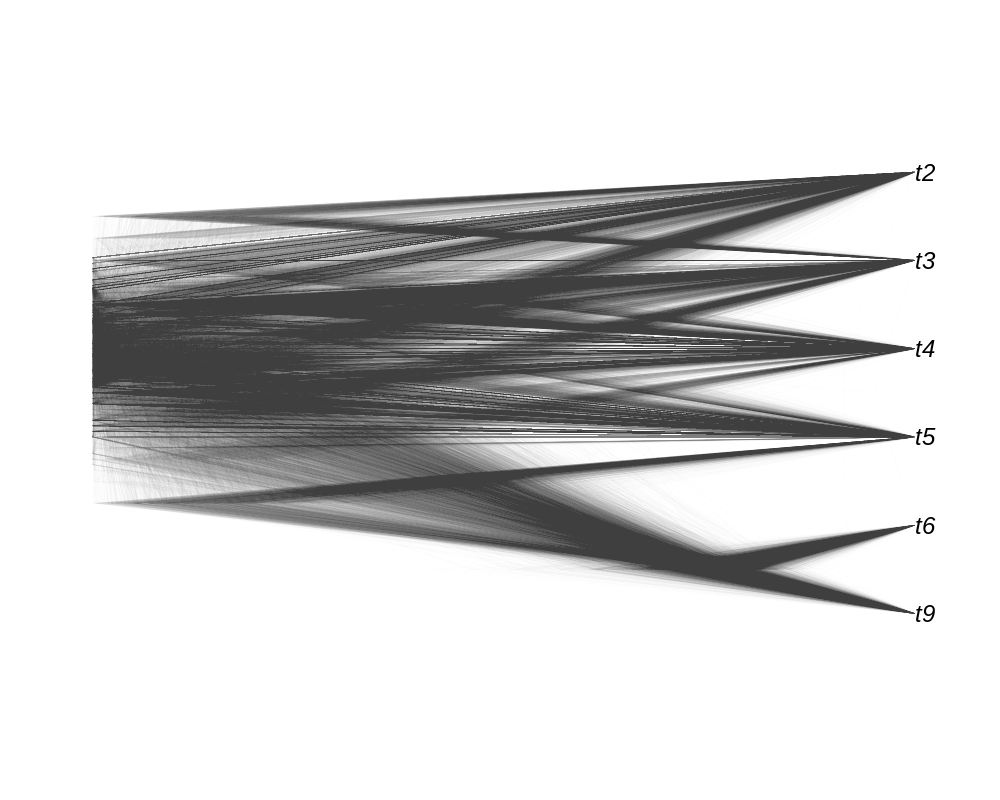
\includegraphics[height=0.3\textheight]{pirouette_example_30/example_30_314/true_posterior_best.png}
    };   
    \node[state] (DB) [below of = CB, rectangle] {
      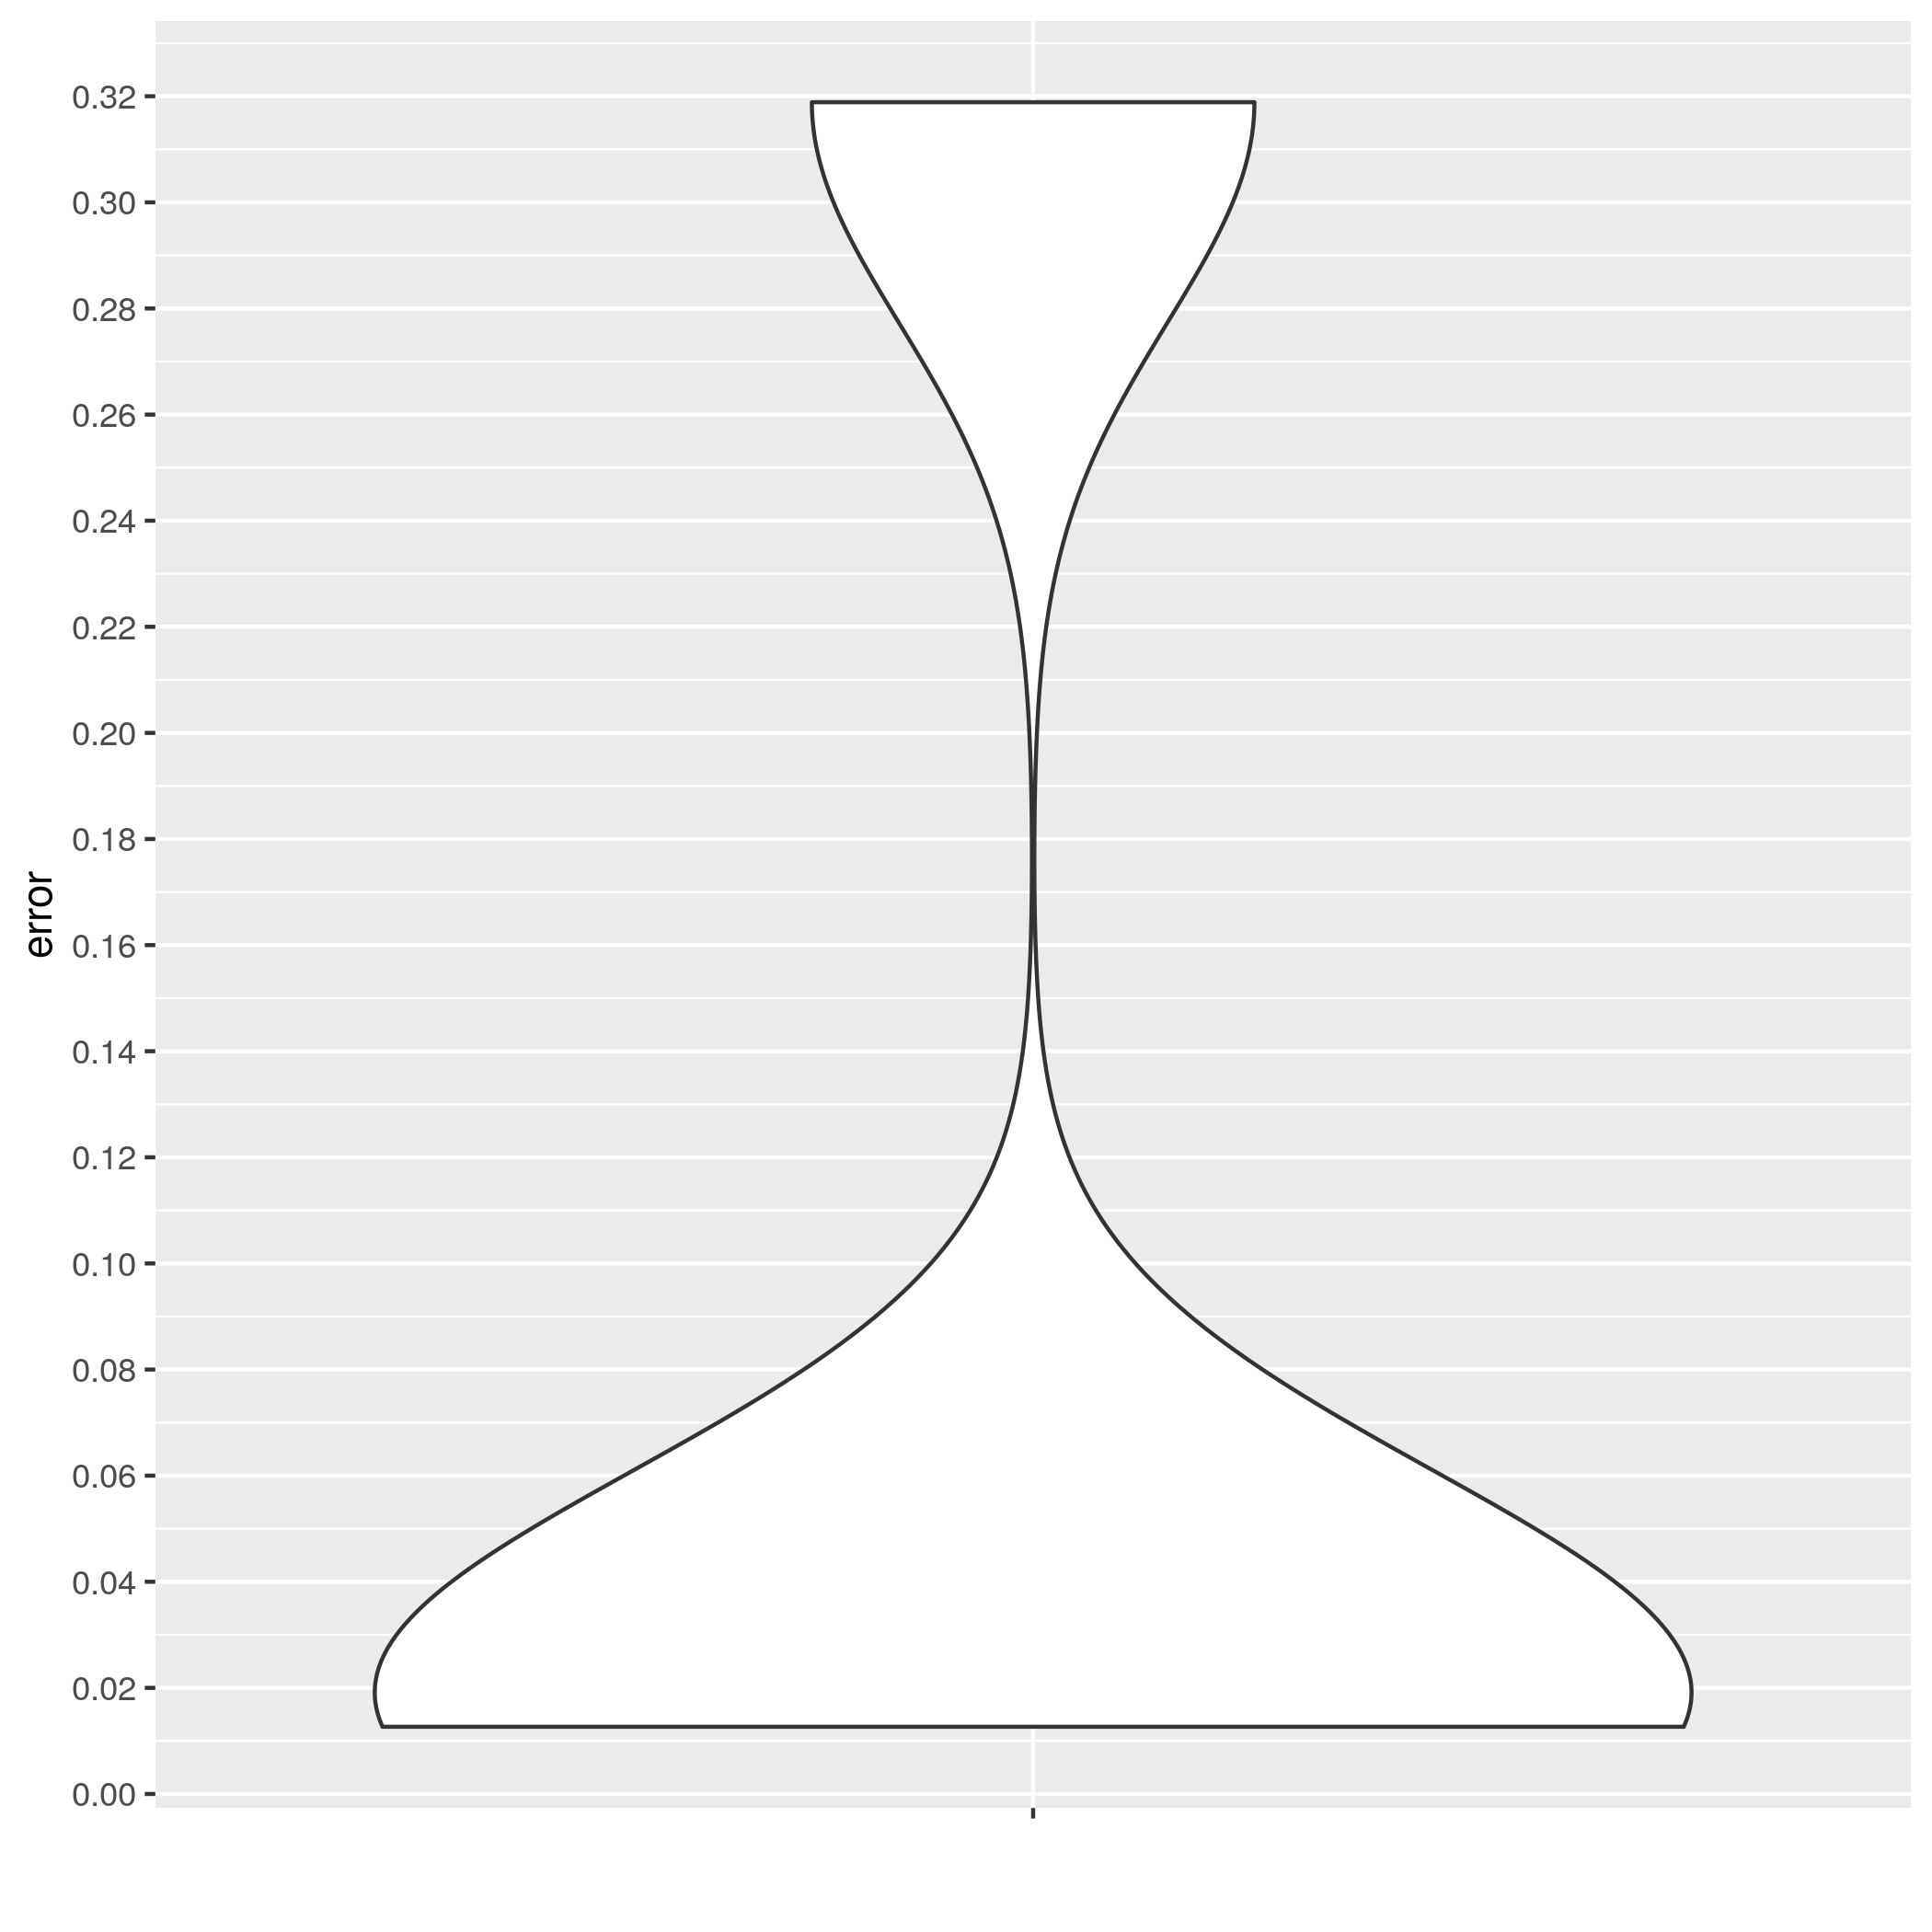
\includegraphics[height=0.3\textheight]{pirouette_example_30/example_30_314/true_error_violin_best.png}
    };   
    \node[state] (AT) [right of = A, rectangle, node distance=0.8\textheight] {
      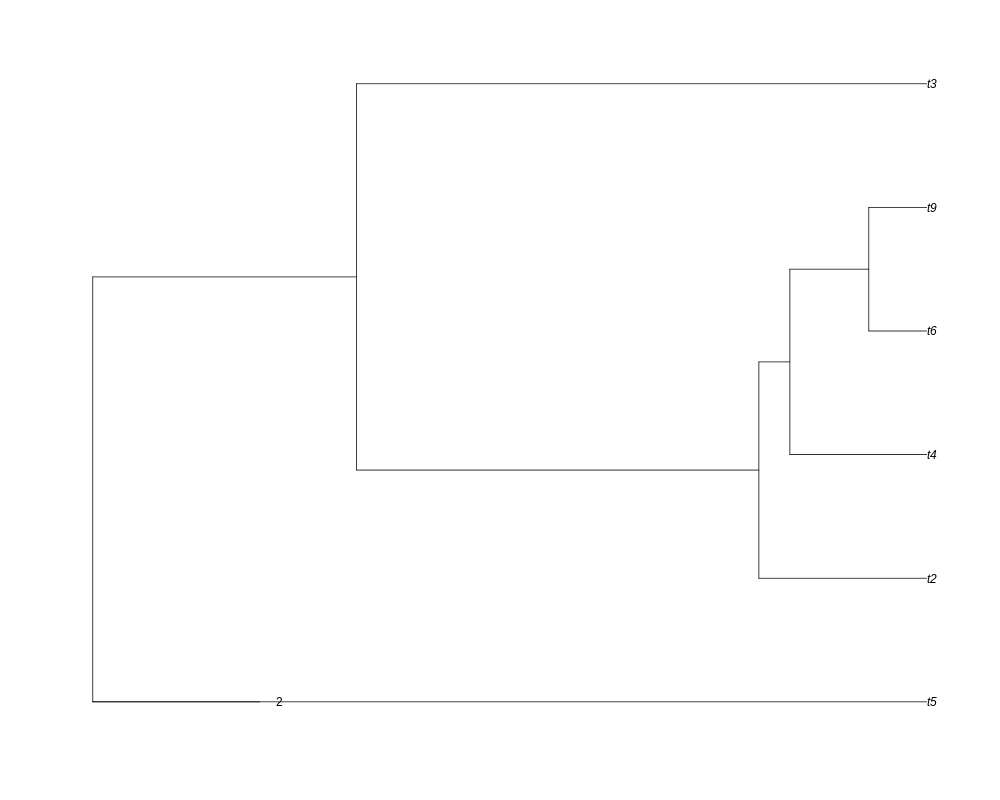
\includegraphics[height=0.4\textheight]{pirouette_example_30/example_30_314/twin_tree.png}
    };   
    \node[state] (BT) [below of = AT, rectangle] {
      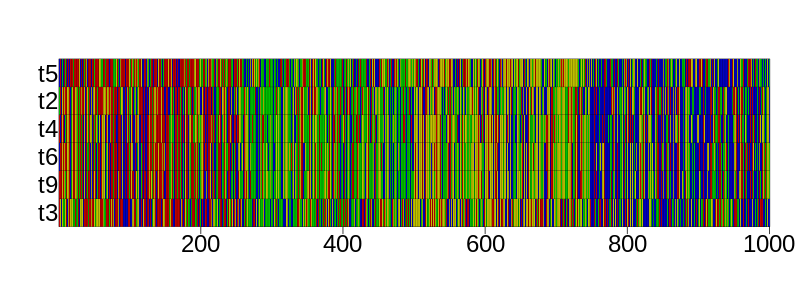
\includegraphics[height=0.25\textheight]{pirouette_example_30/example_30_314/twin_alignment.png}
    };   
    \node[state] (CTG) [right of = CB, rectangle] {
      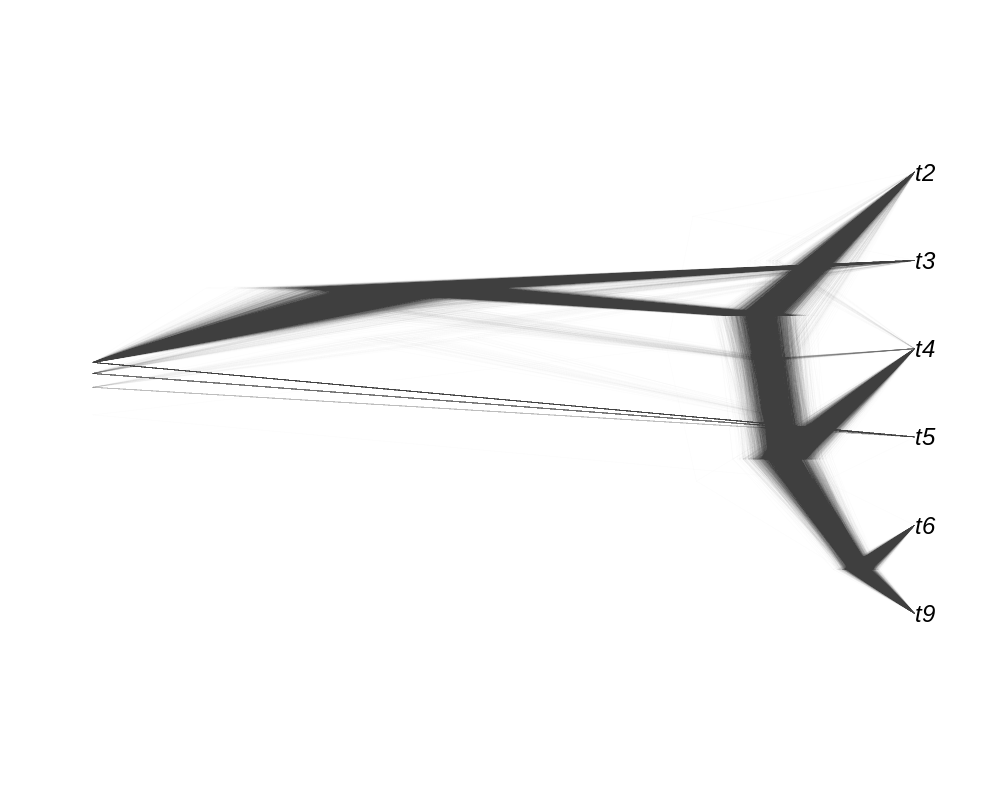
\includegraphics[height=0.3\textheight]{pirouette_example_30/example_30_314/twin_posterior_gen.png}
    };   
    \node[state] (DTG) [below of = CTG, rectangle] {
      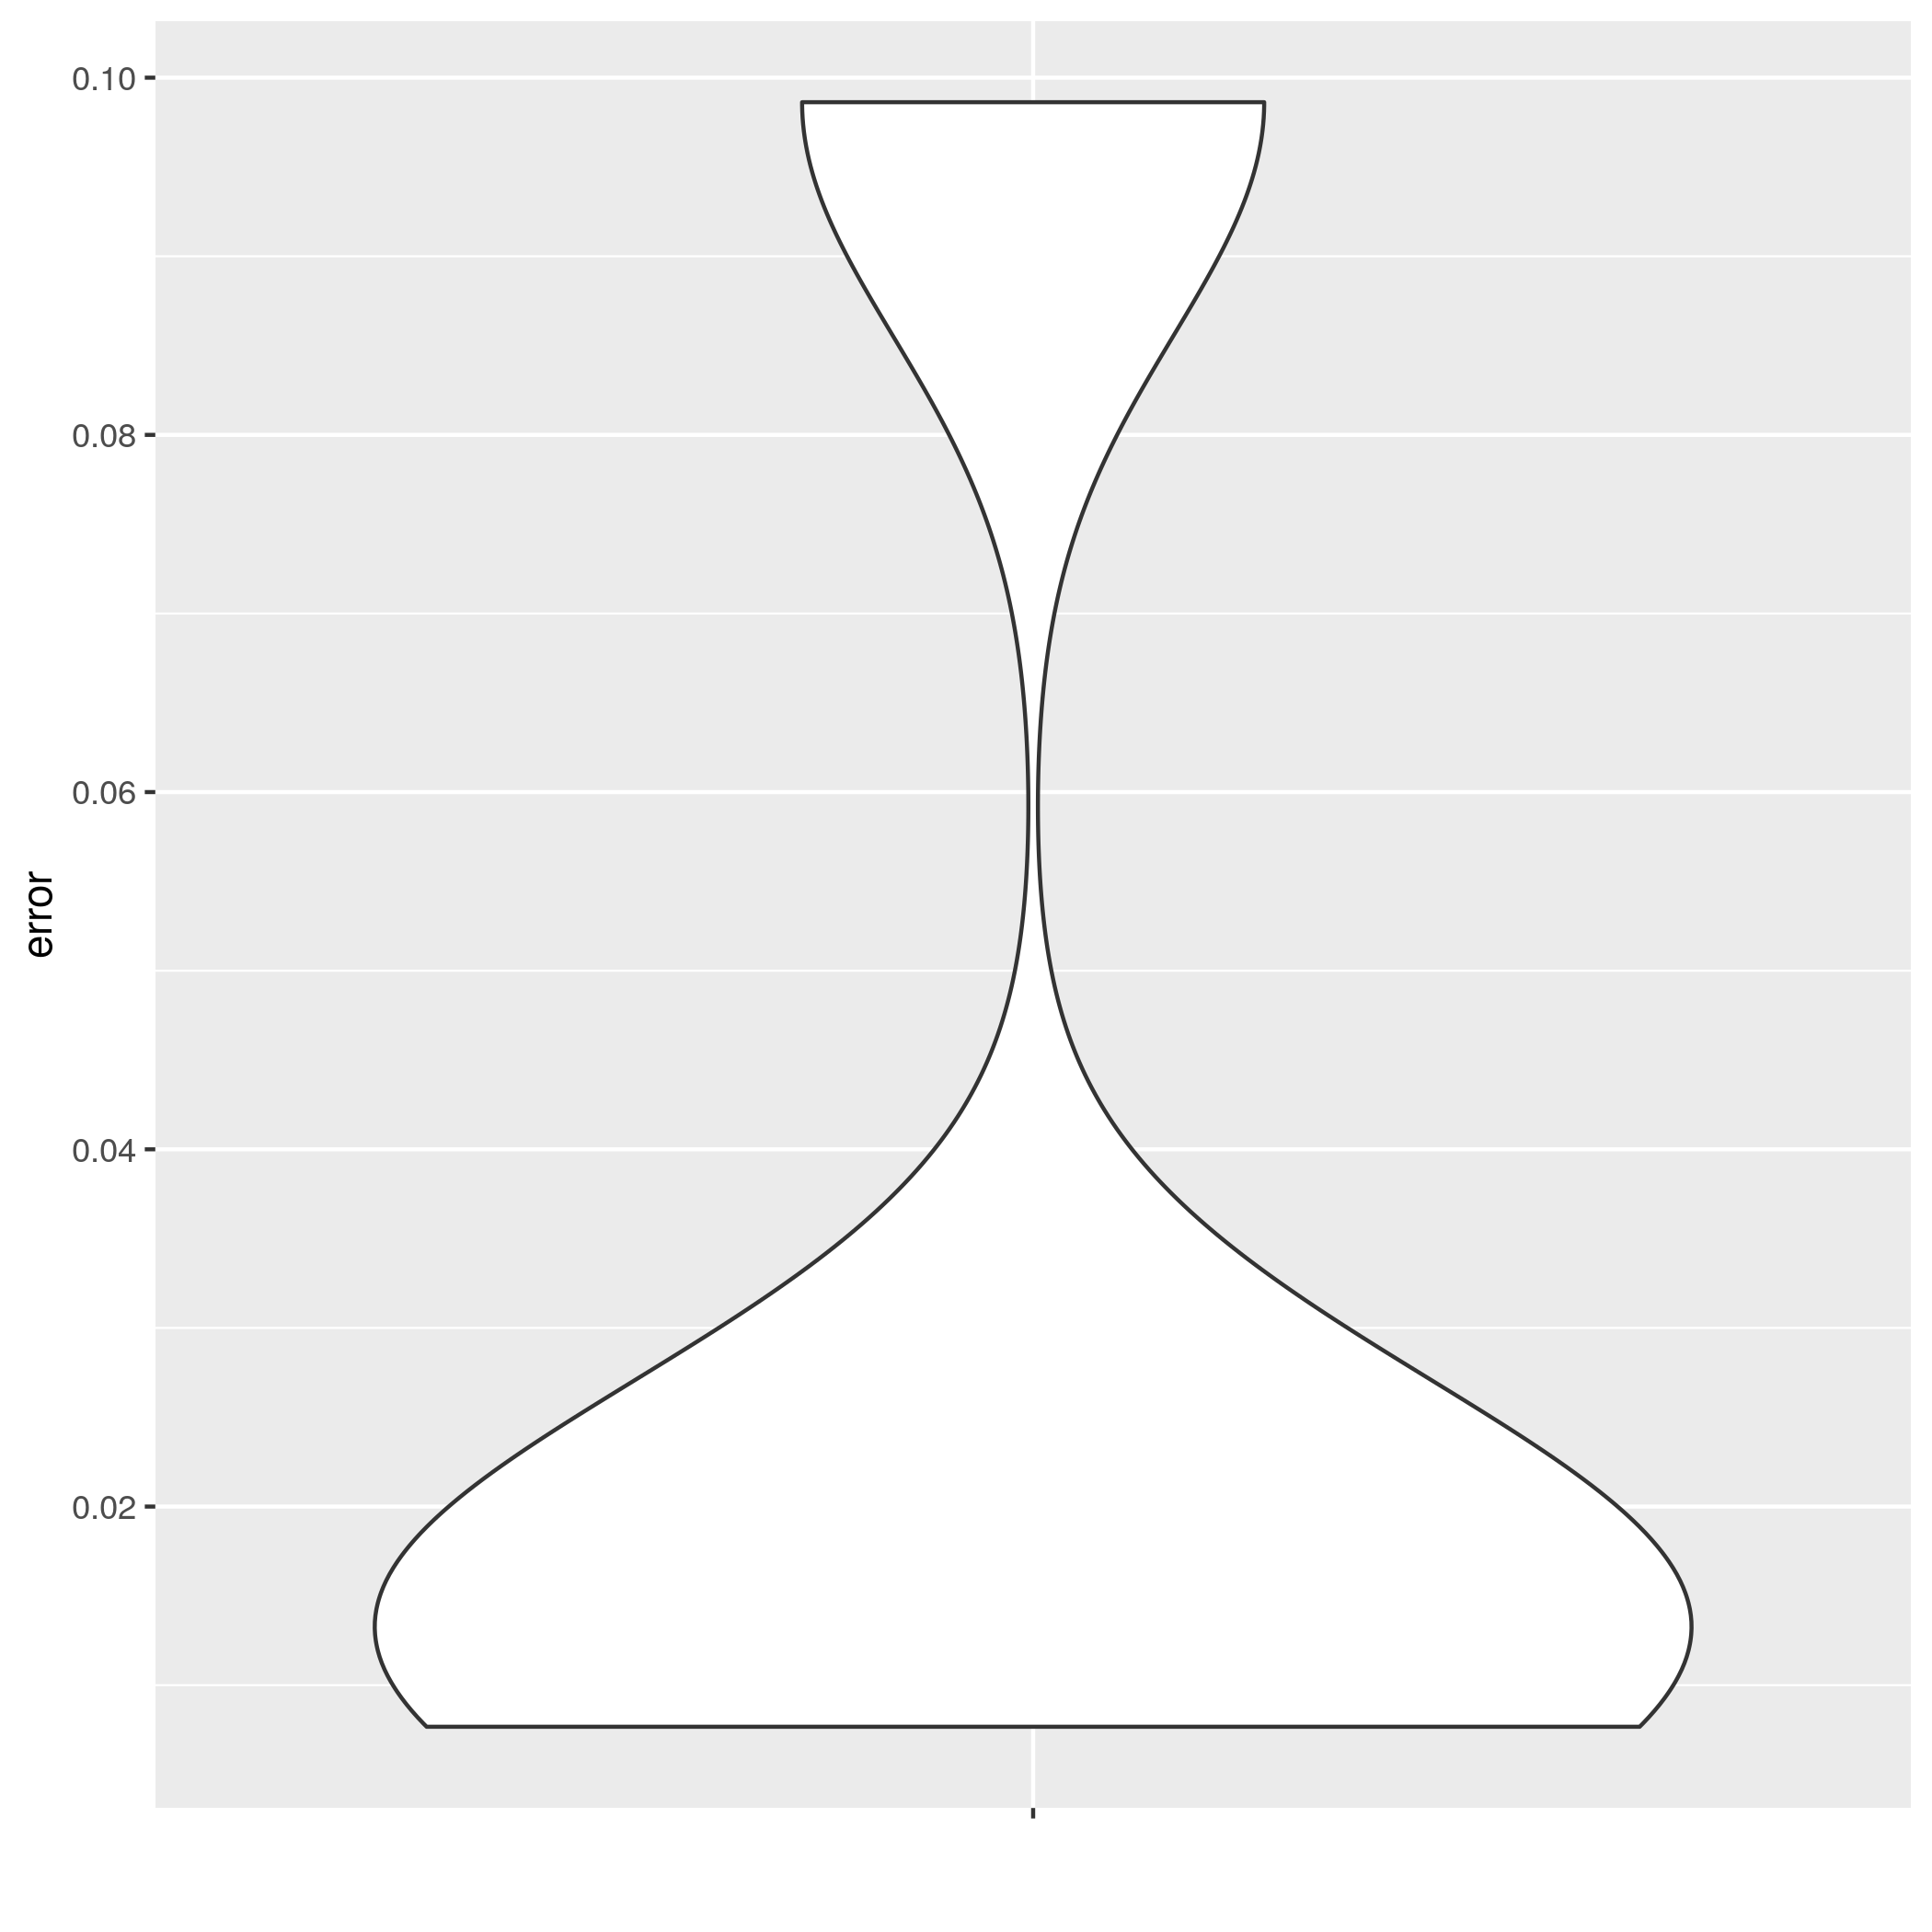
\includegraphics[height=0.3\textheight]{pirouette_example_30/example_30_314/twin_error_violin_gen.png}
    };   
    \node[state] (CTB) [right of = CTG, rectangle] {
      
\includegraphics[height=0.3\textheight]{pirouette_example_30/example_30_314/twin_posterior_best.png}
    };   
    \node[state] (DTB) [below of = CTB, rectangle] {
      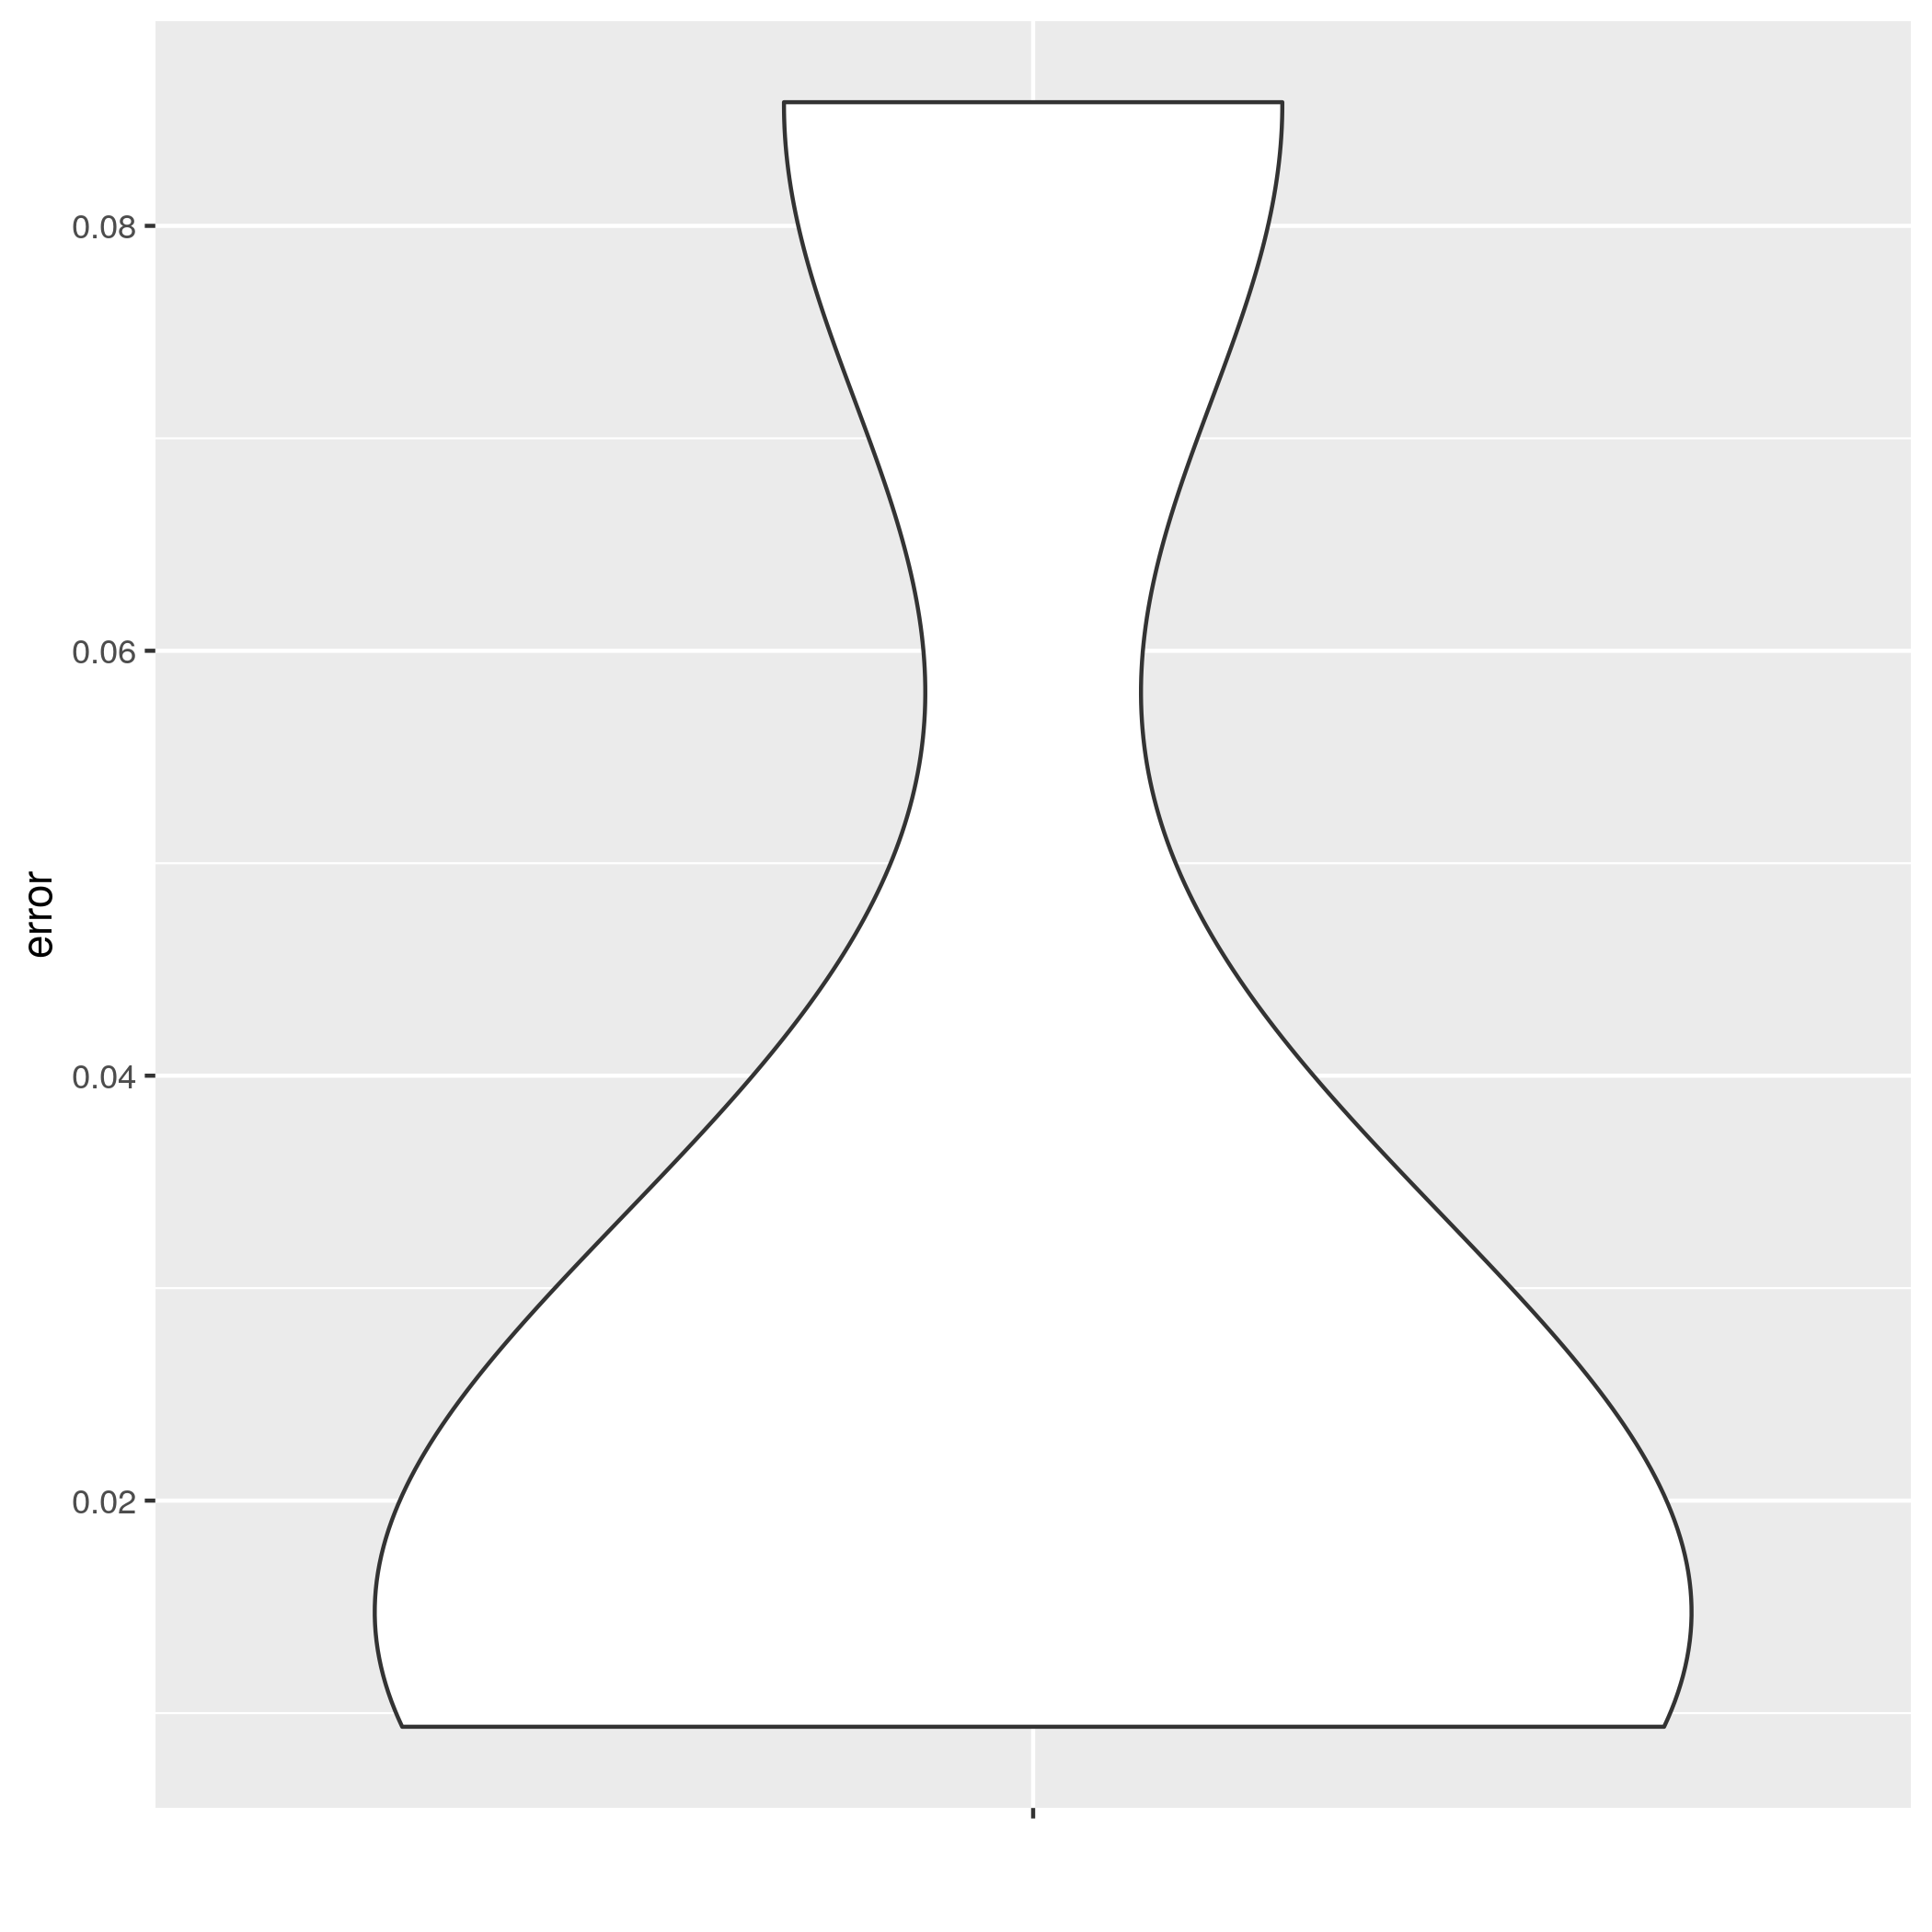
\includegraphics[height=0.3\textheight]{pirouette_example_30/example_30_314/twin_error_violin_best.png}
    };   
    \path 
      (O) edge [anchor = south] node {} (A)
      (A) edge [anchor = south] node {} (B)
      (B) edge [anchor = south] node {} (CG)
      (CG) edge [anchor = south] node {} (DG)
      (B) edge [anchor = south east] node {} (CB)
      (CB) edge [anchor = south] node {} (DB)
      (A) edge [anchor = east] node {} (AT)
      (AT) edge [anchor = south] node {} (BT)
      (BT) edge [anchor = south east] node {} (CTG)
      (CTG) edge [anchor = south] node {} (DTG)
      (BT) edge [anchor = south] node {} (CTB)
      (CTB) edge [anchor = south] node {} (DTB)
    ; 
    \end{tikzpicture}
  }
  \label{fig:example_30_full_pipeline}
  \caption{Comparing to background noise: full pipeline}
\end{figure}
%%%%%%%%%%%%%%%%%%%%%%%%%%%%%%%%%%%%%%%%%%%%%%%%%%%%%%%%%%%%%%%%%%%%%%%%%%%%%%%%

\input{pirouette_example_30/example_30_314/esses_gen.latex}

\input{pirouette_example_30/example_30_314/esses_best.latex}

\input{pirouette_example_30/example_30_314/esses_twin_gen.latex}

\input{pirouette_example_30/example_30_314/esses_twin_best.latex}

\input{pirouette_example_30/example_30_314/evidence_true.latex}

\input{pirouette_example_30/example_30_314/evidence_twin.latex}

%%%%%%%%%%%%%%%%%%%%%%%%%%%%%%%%%%%%%%%%%%%%%%%%%%%%%%%%%%%%%%%%%%%%%%%%%%%%%%%%
\subsection{Using a distribution of trees}
\label{subsec:distribution}
%%%%%%%%%%%%%%%%%%%%%%%%%%%%%%%%%%%%%%%%%%%%%%%%%%%%%%%%%%%%%%%%%%%%%%%%%%%%%%%%

This subsection extends the main example, by using multiple (instead of
one) trees. These trees are produced by running a DD tree simulation
with the same parameters as the main example.

The code used in this part of the article can be found at 
\url{https://github.com/richelbilderbeek/pirouette_example_28}.

\begin{figure}[H]
  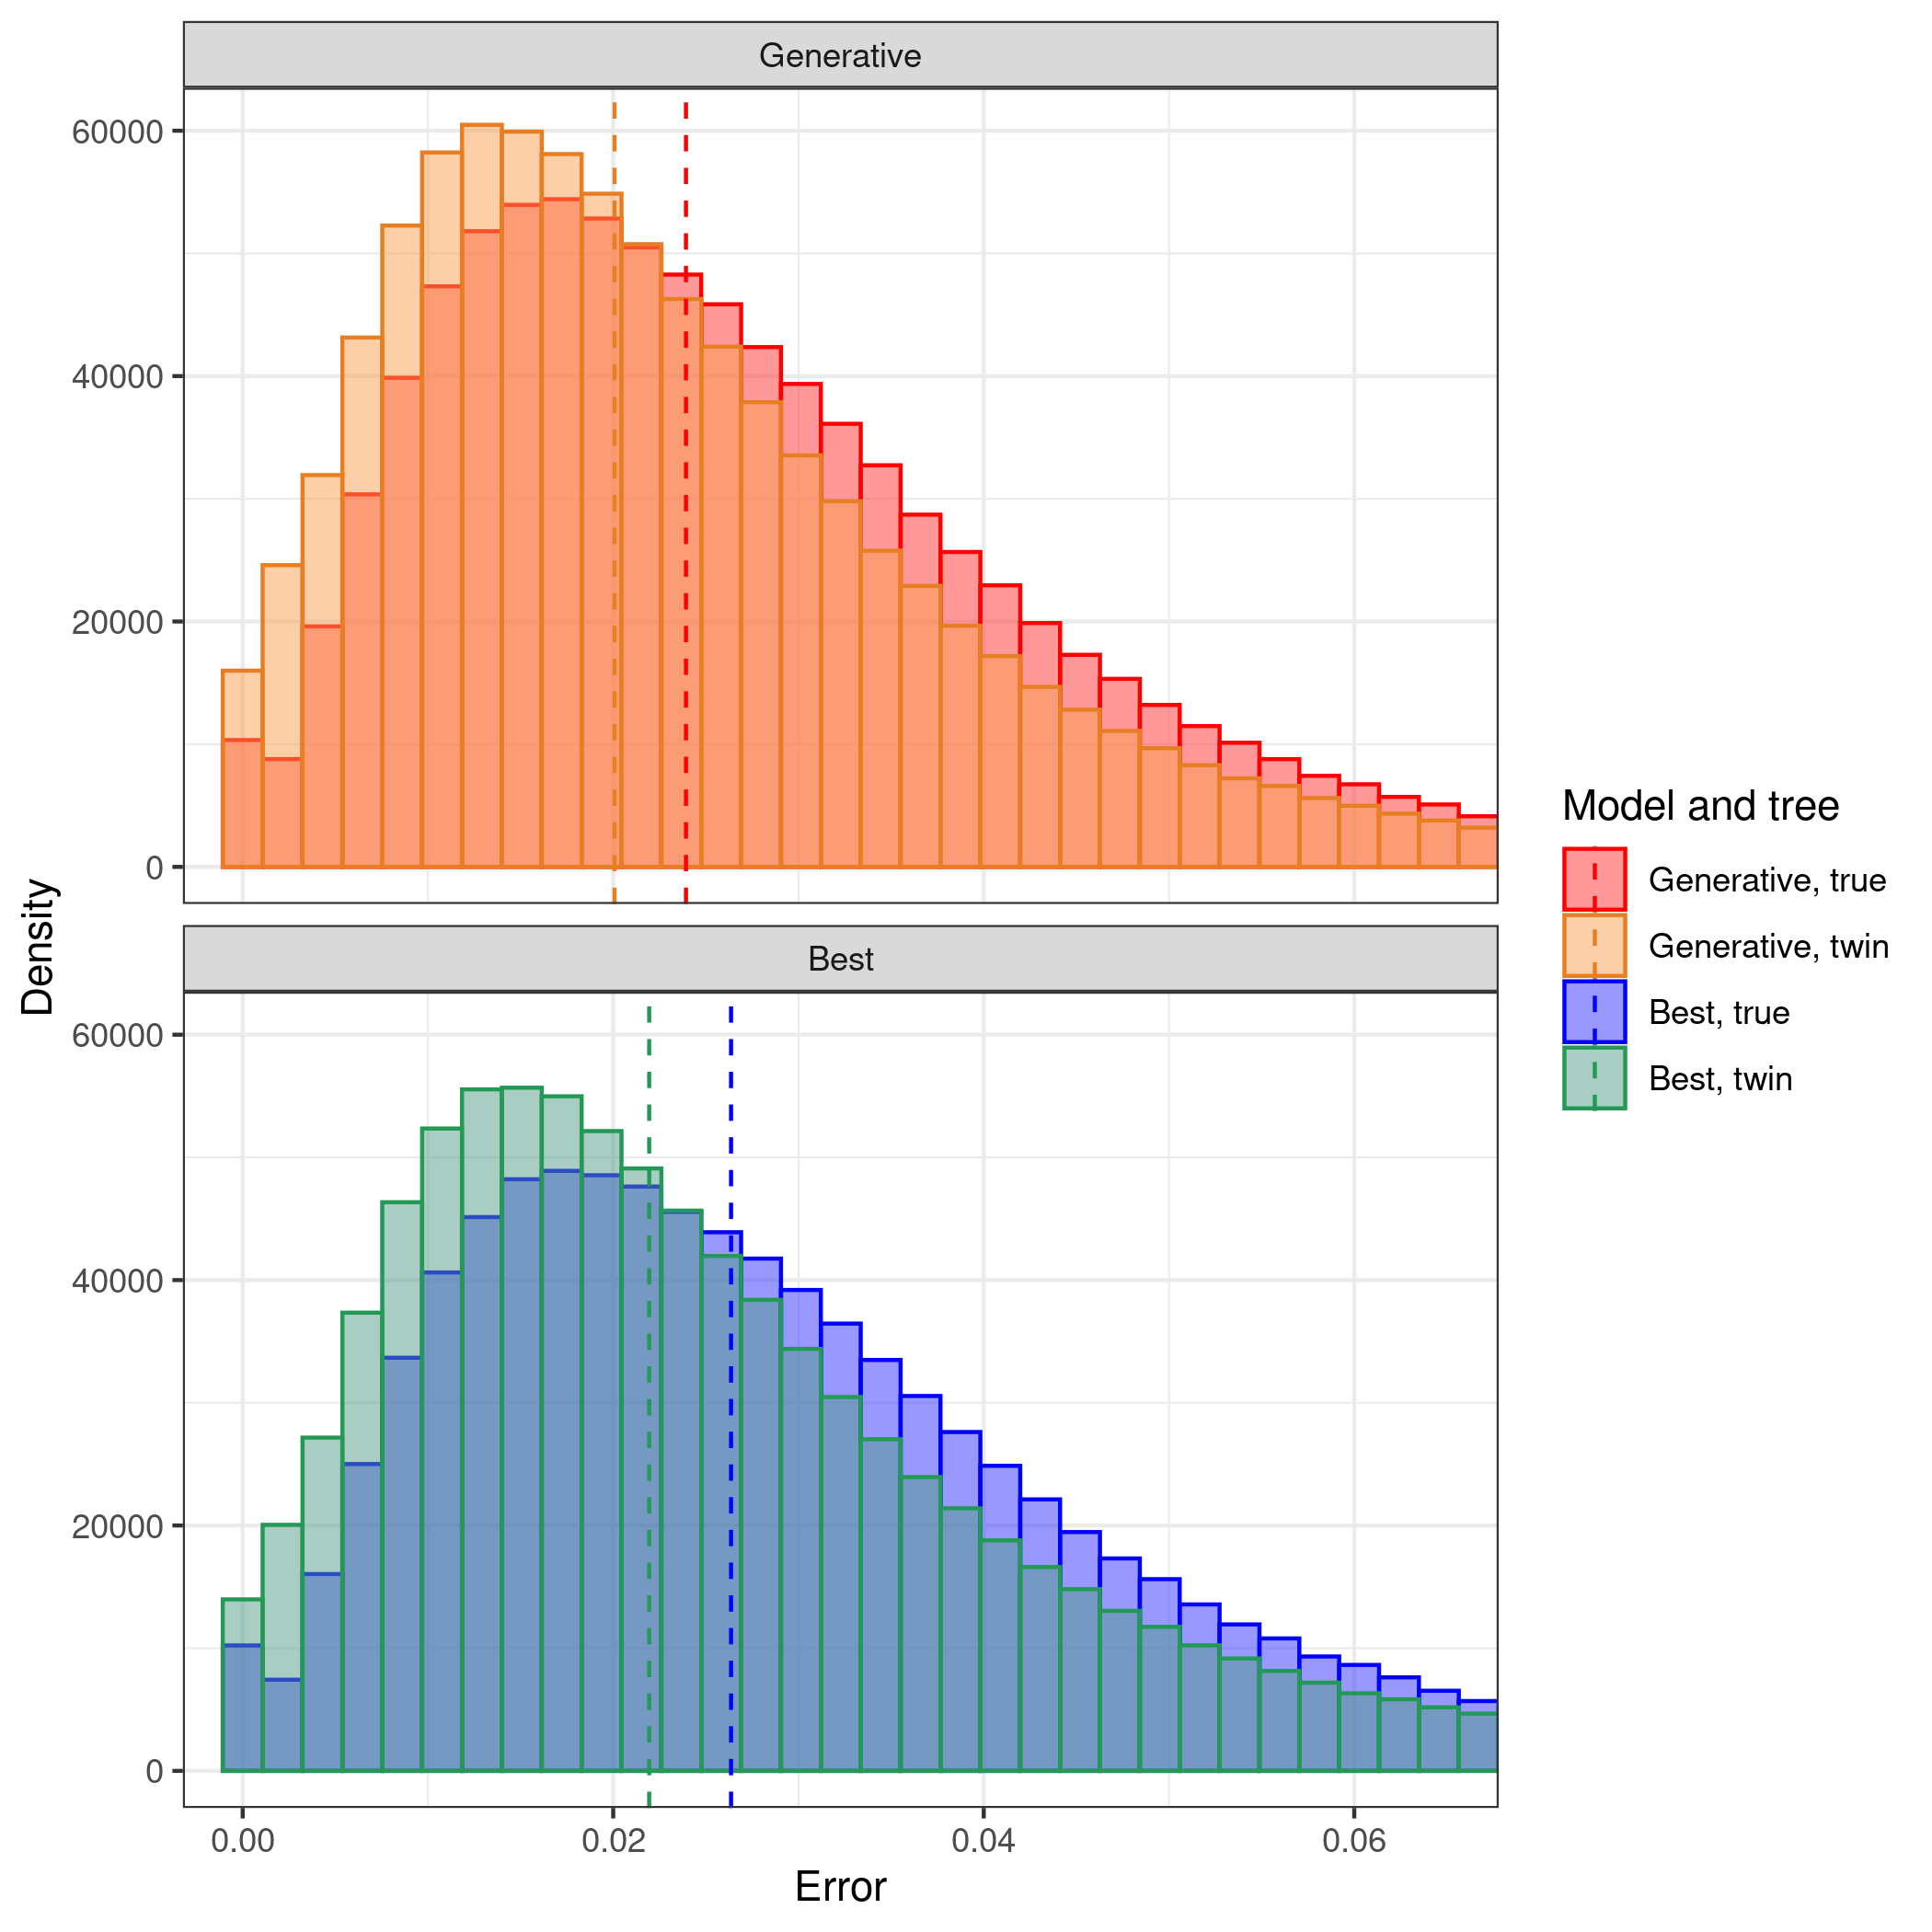
\includegraphics[width=\textwidth]{pirouette_example_28/errors.png}
  \caption{Error distribution from a distribution of trees}
\end{figure}

%%%%%%%%%%%%%%%%%%%%%%%%%%%%%%%%%%%%%%%%%%%%%%%%%%%%%%%%%%%%%%%%%%%%%%%%%%%%%%%%
\subsection{The effect of the number of taxa}
\label{subsec:n_taxa}
%%%%%%%%%%%%%%%%%%%%%%%%%%%%%%%%%%%%%%%%%%%%%%%%%%%%%%%%%%%%%%%%%%%%%%%%%%%%%%%%

The main example uses 6 taxa. Here, we show the same results as the main example,
except for a varying number of taxa.

The code used in this part of the article can be found at 
\url{https://github.com/richelbilderbeek/pirouette_example_28} (6 taxa, main example),
\url{https://github.com/richelbilderbeek/pirouette_example_32} (12 taxa),
\url{https://github.com/richelbilderbeek/pirouette_example_33} (24 taxa),
\url{https://github.com/richelbilderbeek/pirouette_example_41} (32 taxa),
\url{https://github.com/richelbilderbeek/pirouette_example_42} (40 taxa). 

\begin{figure}[H]
  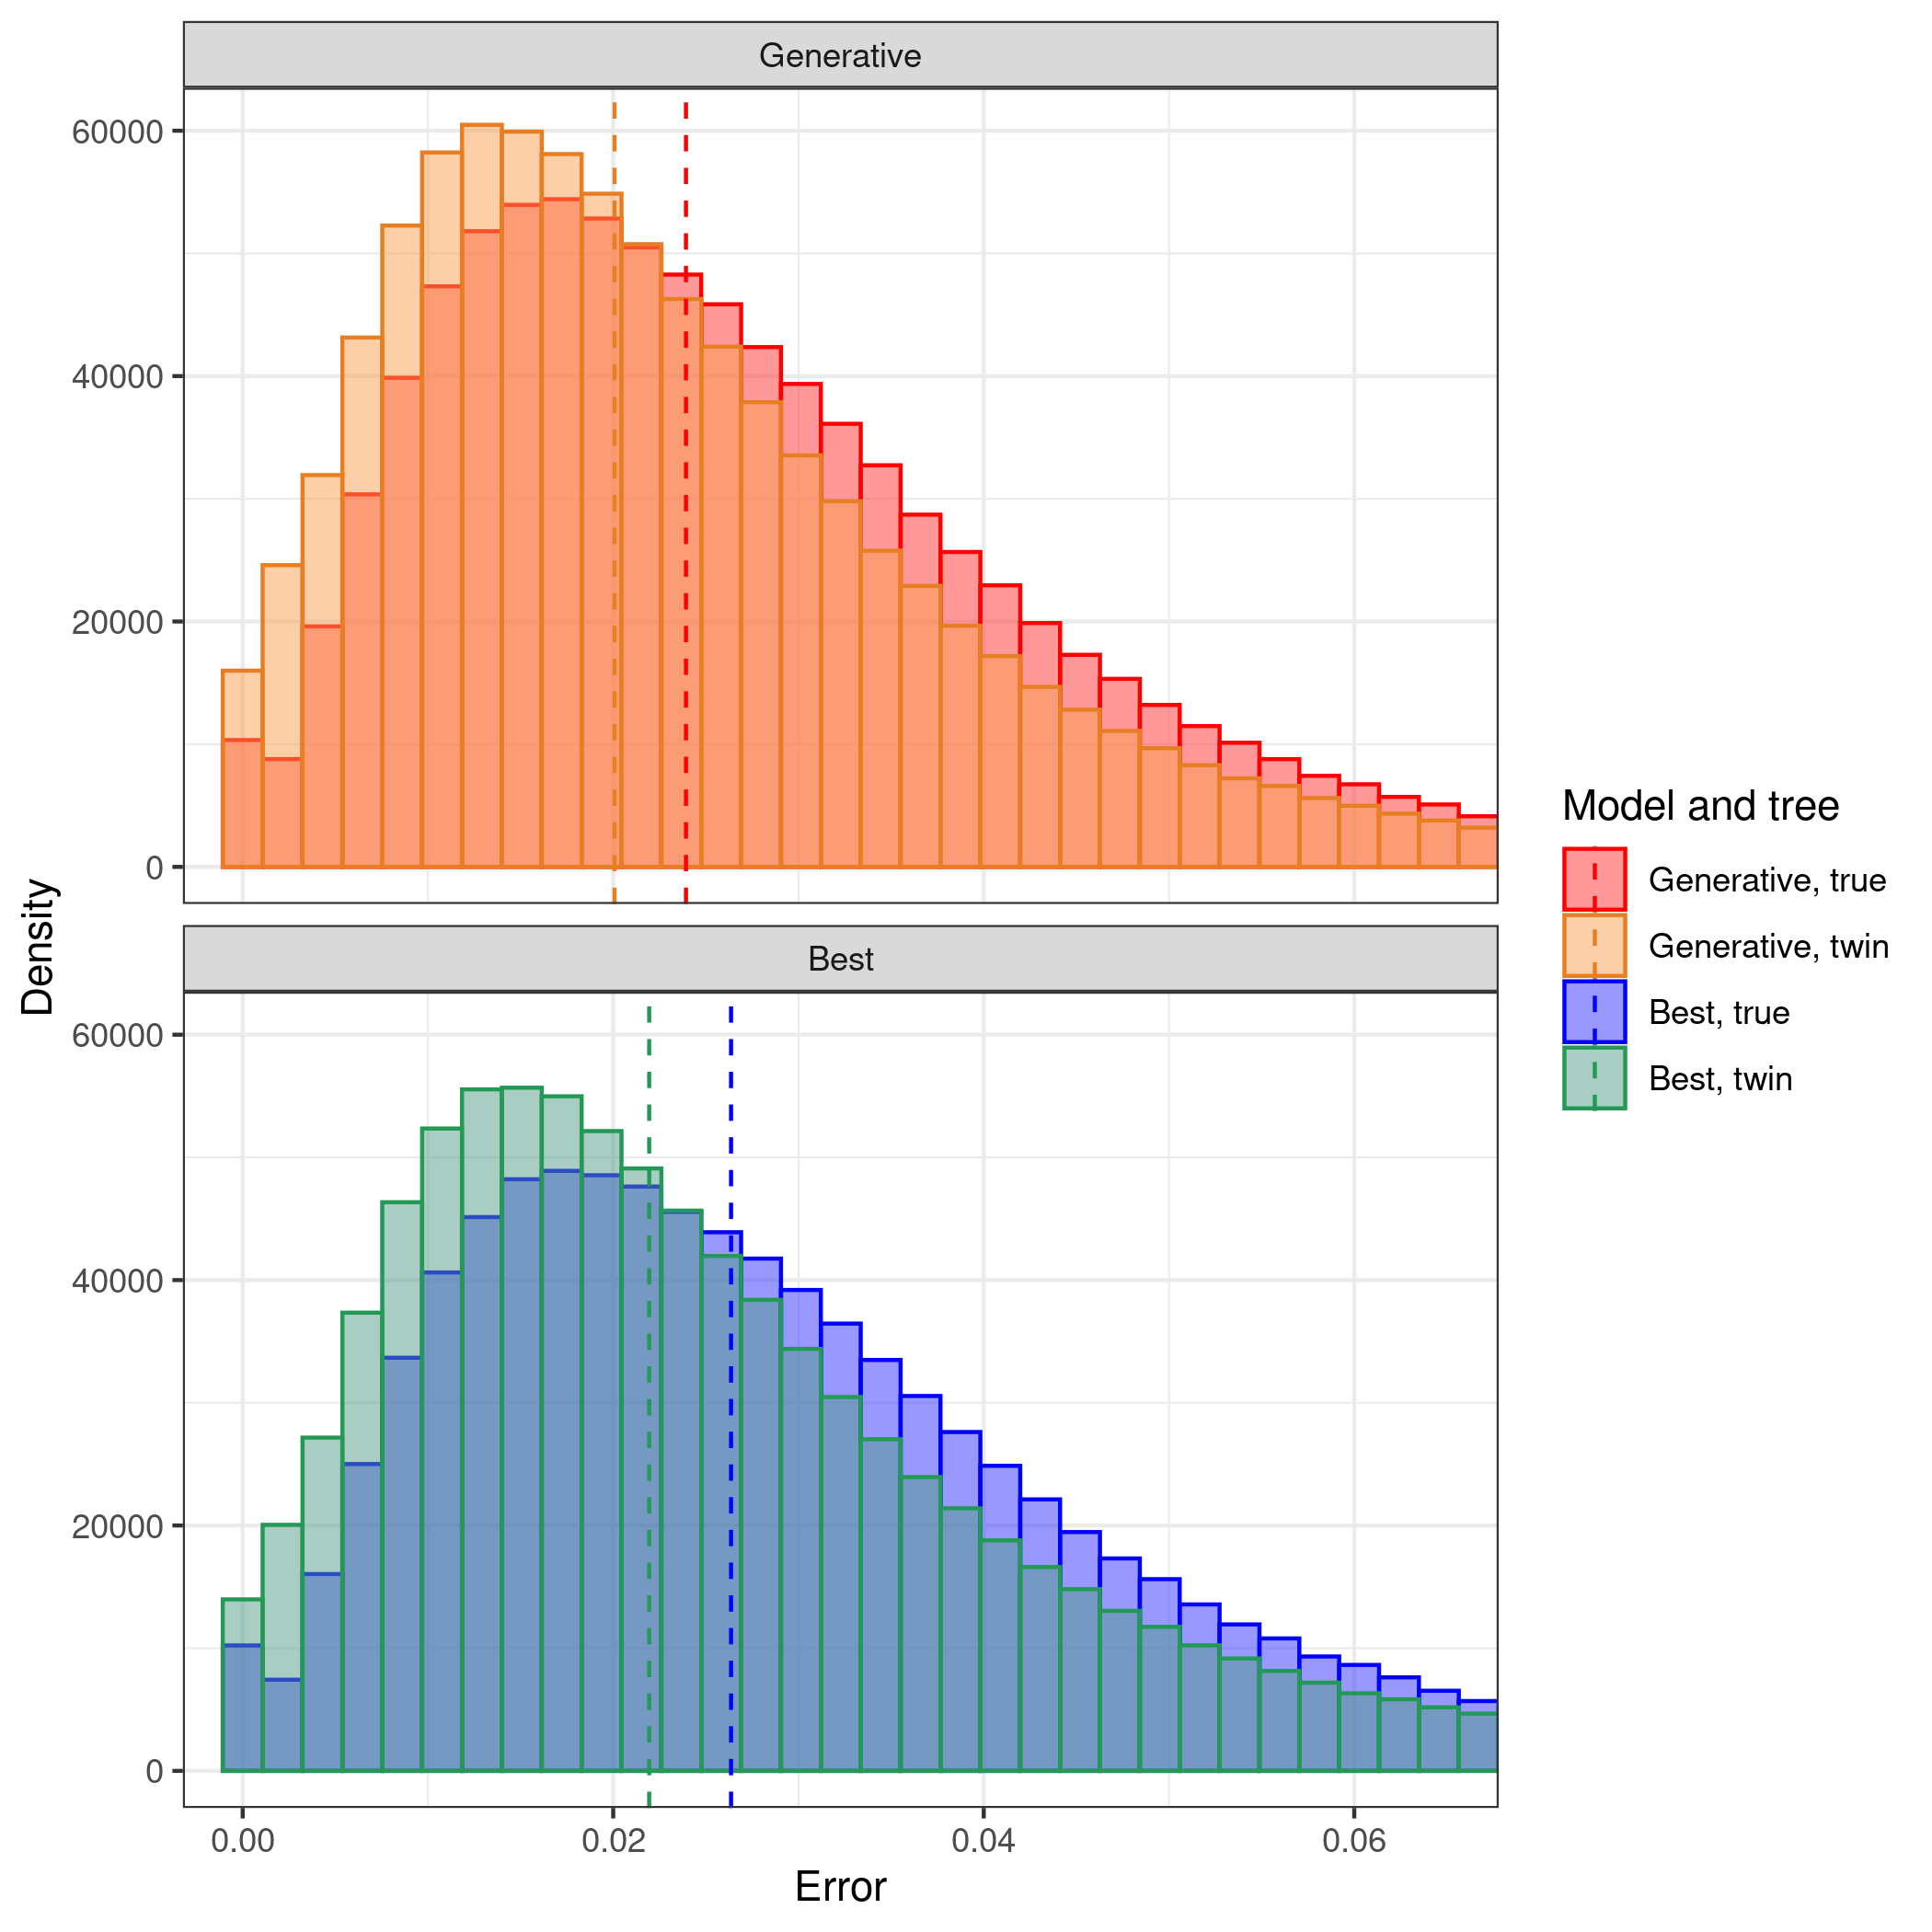
\includegraphics[width=\textwidth]{pirouette_example_28/errors.png}
  \caption{6 taxa, 16 hours, main example}
\end{figure}

\begin{figure}[H]
  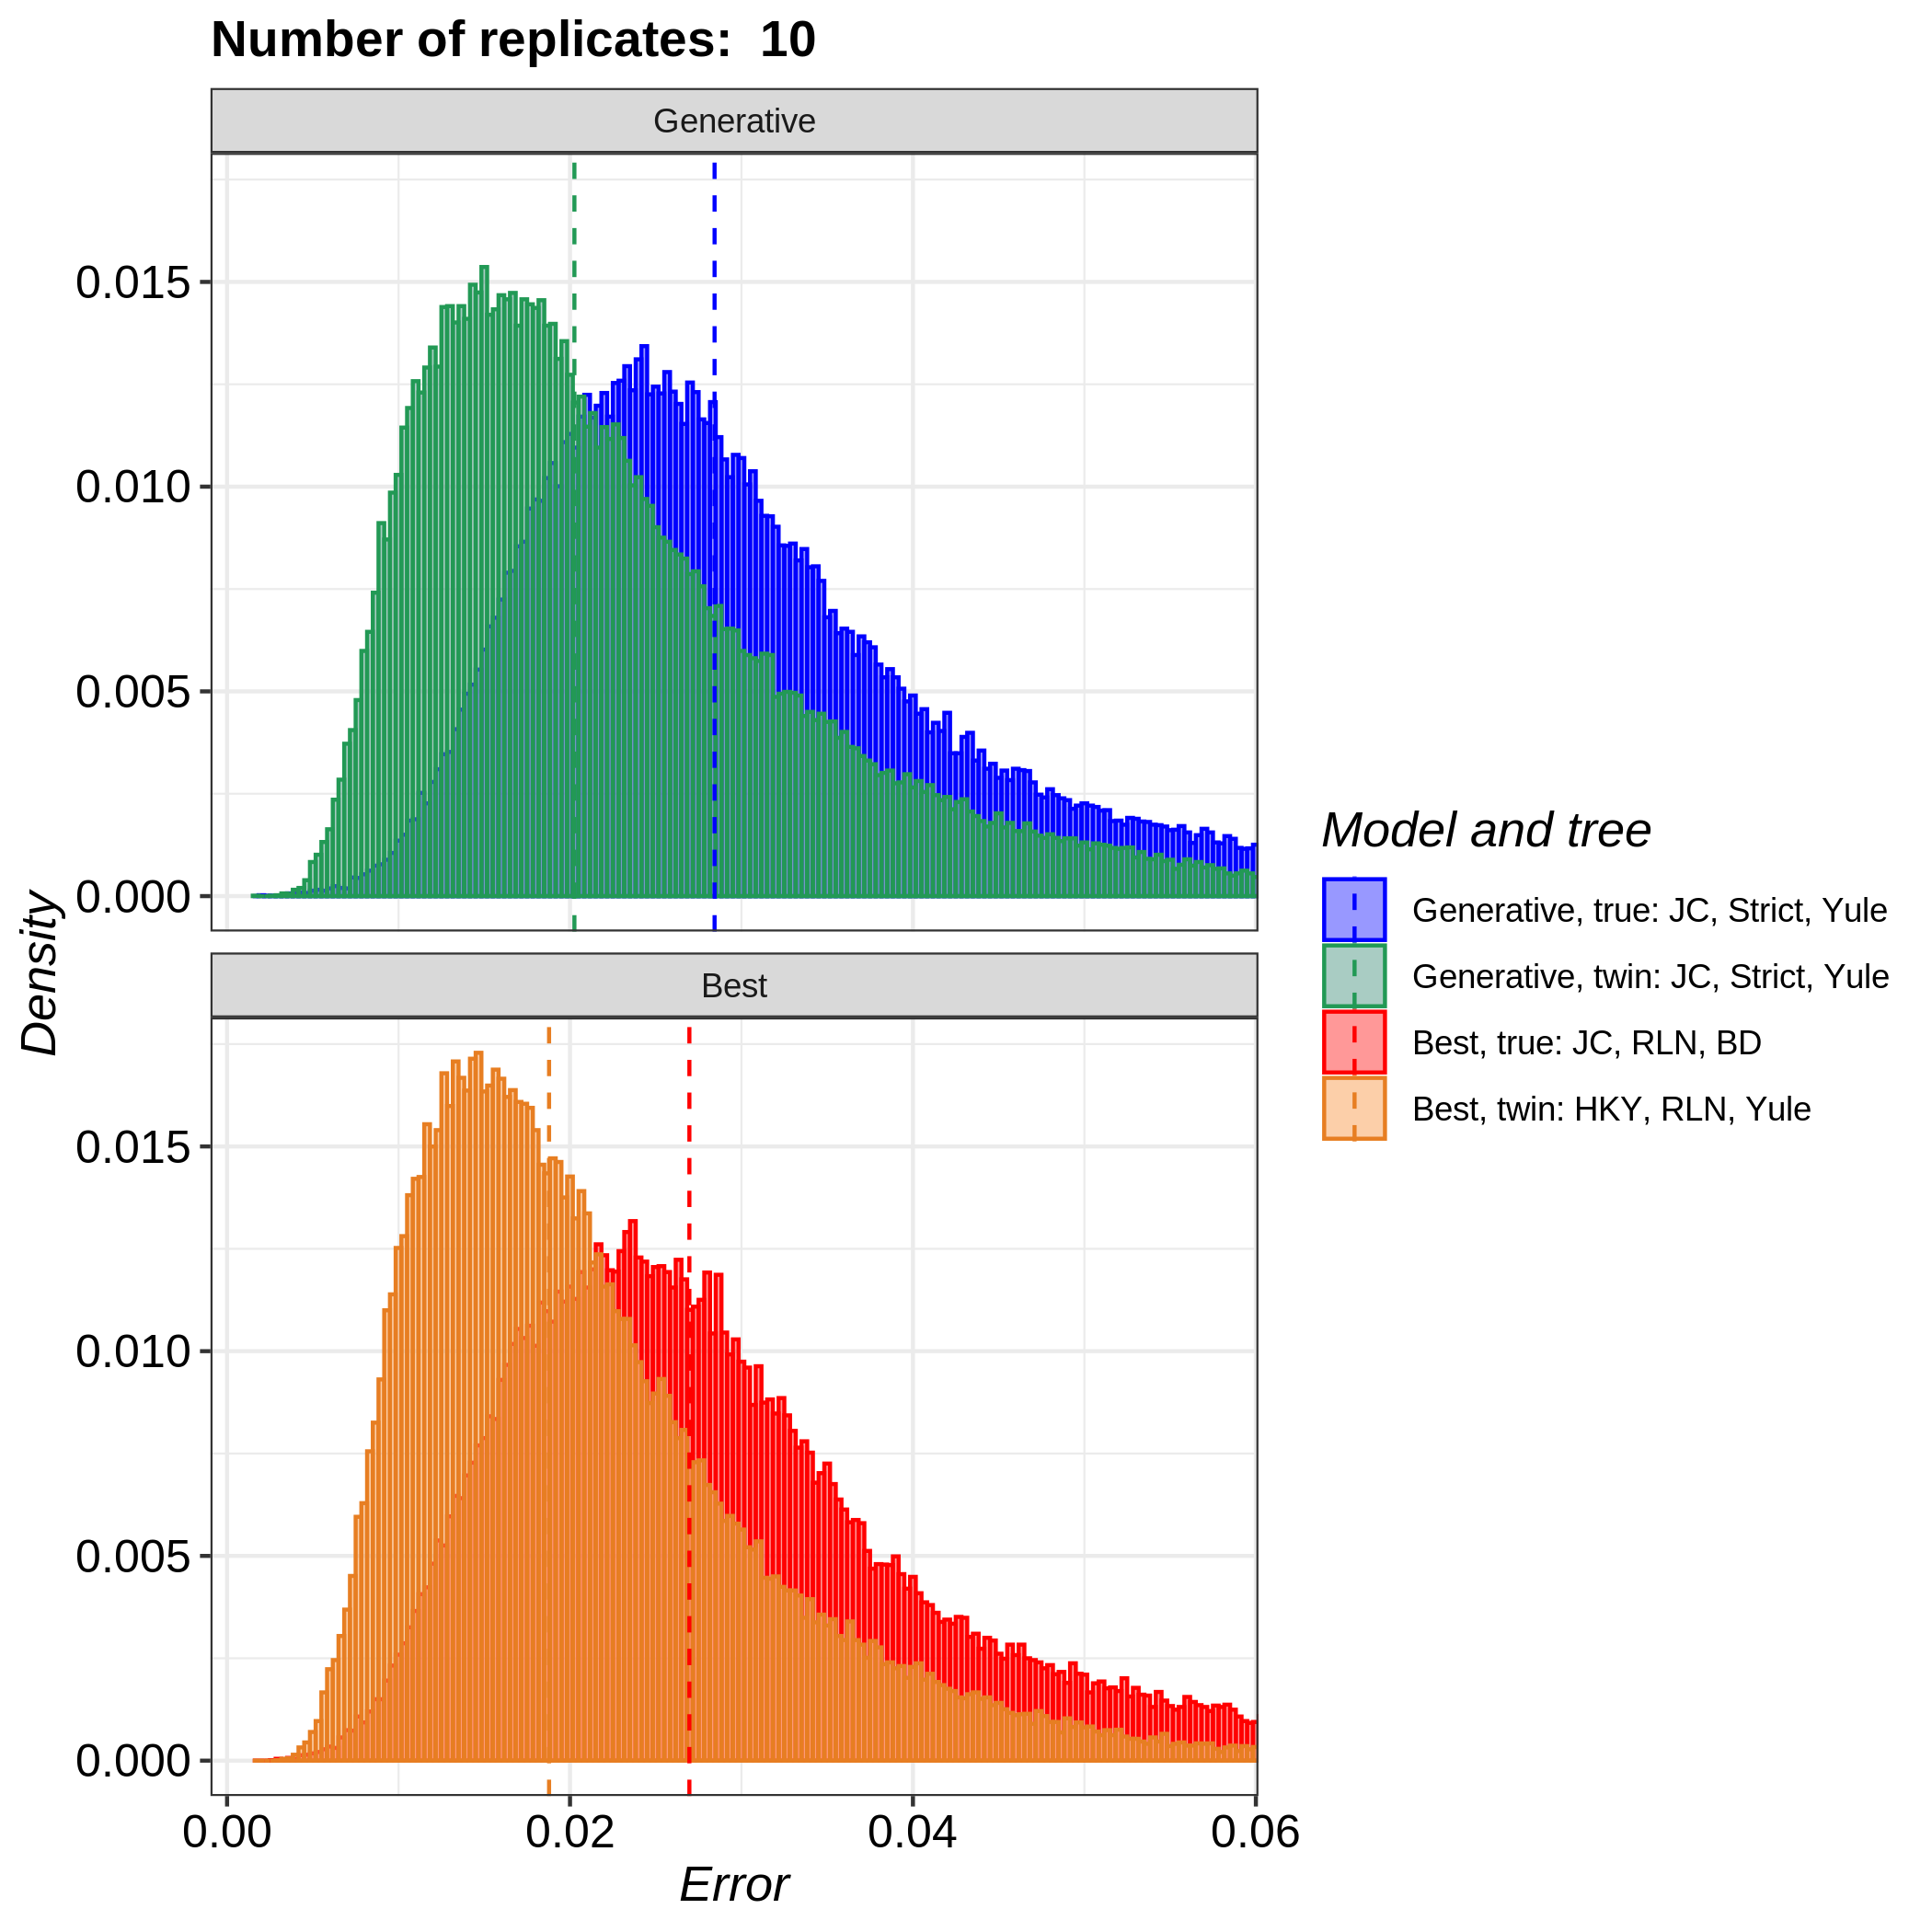
\includegraphics[width=\textwidth]{pirouette_example_32/errors.png}
  \caption{12 taxa, 19 hours}
\end{figure}

\begin{figure}[H]
  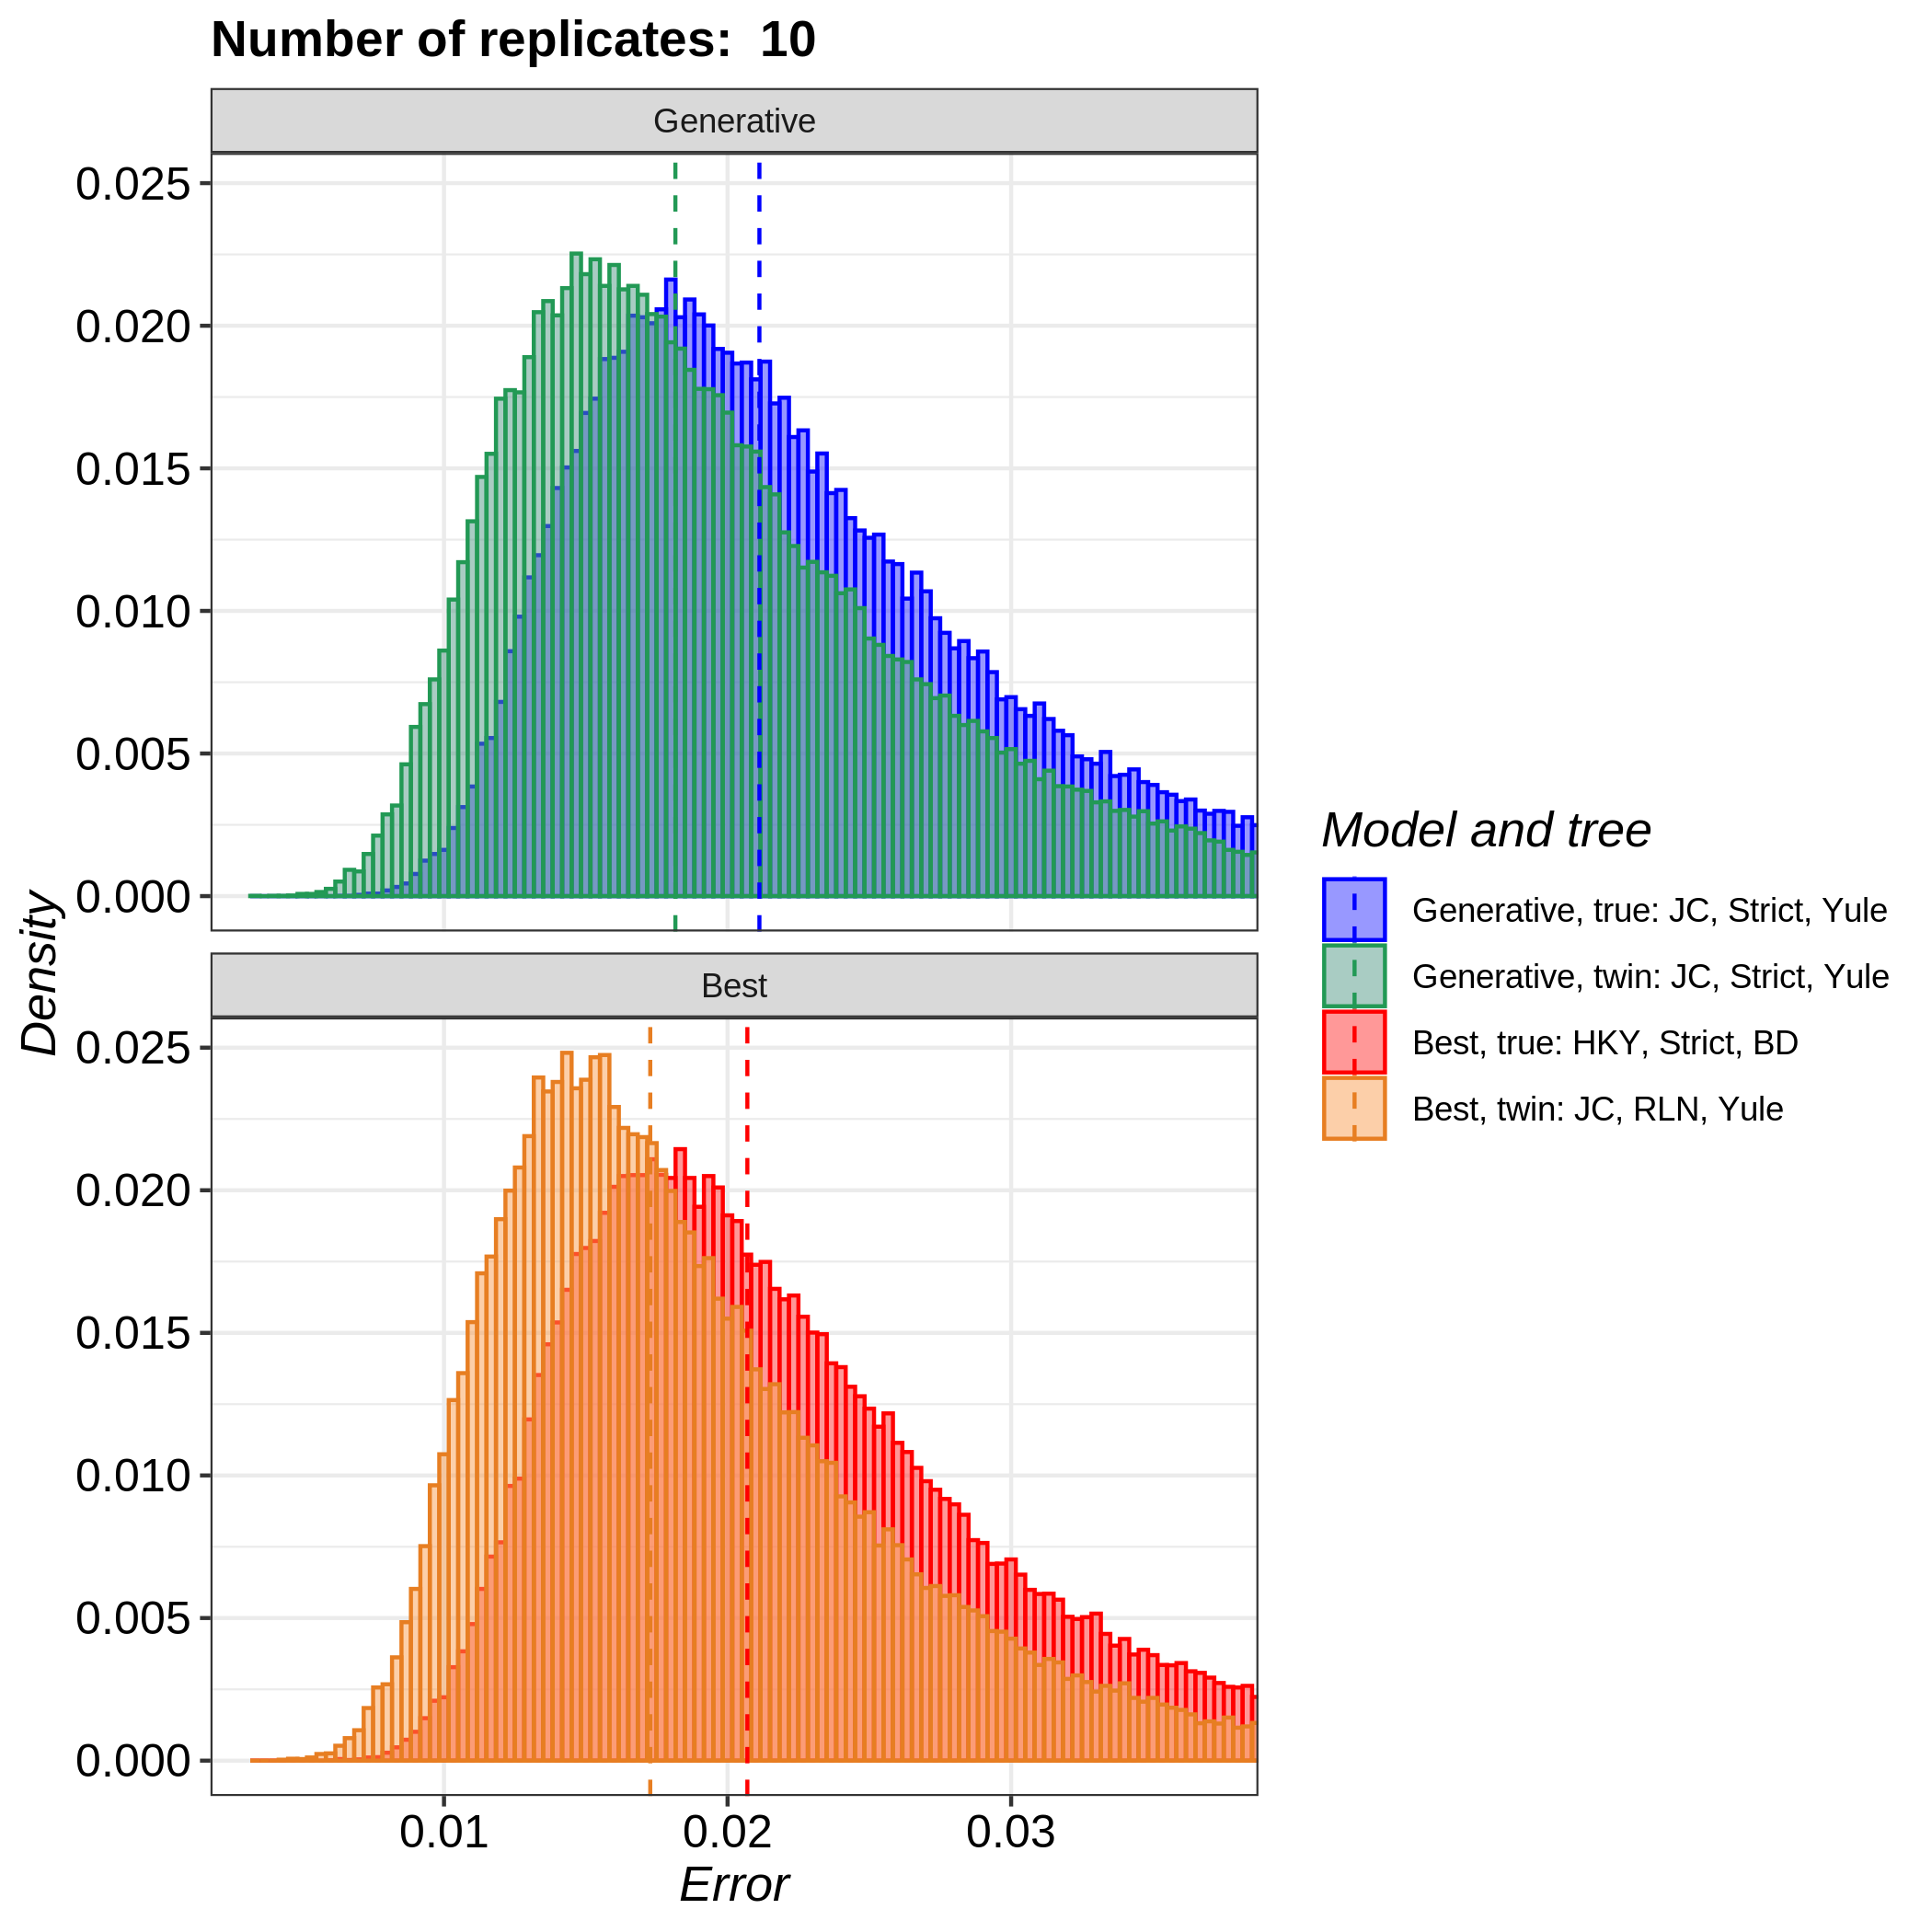
\includegraphics[width=\textwidth]{pirouette_example_33/errors.png}
  \caption{24 taxa, 28 hours}
\end{figure}

\begin{figure}[H]
  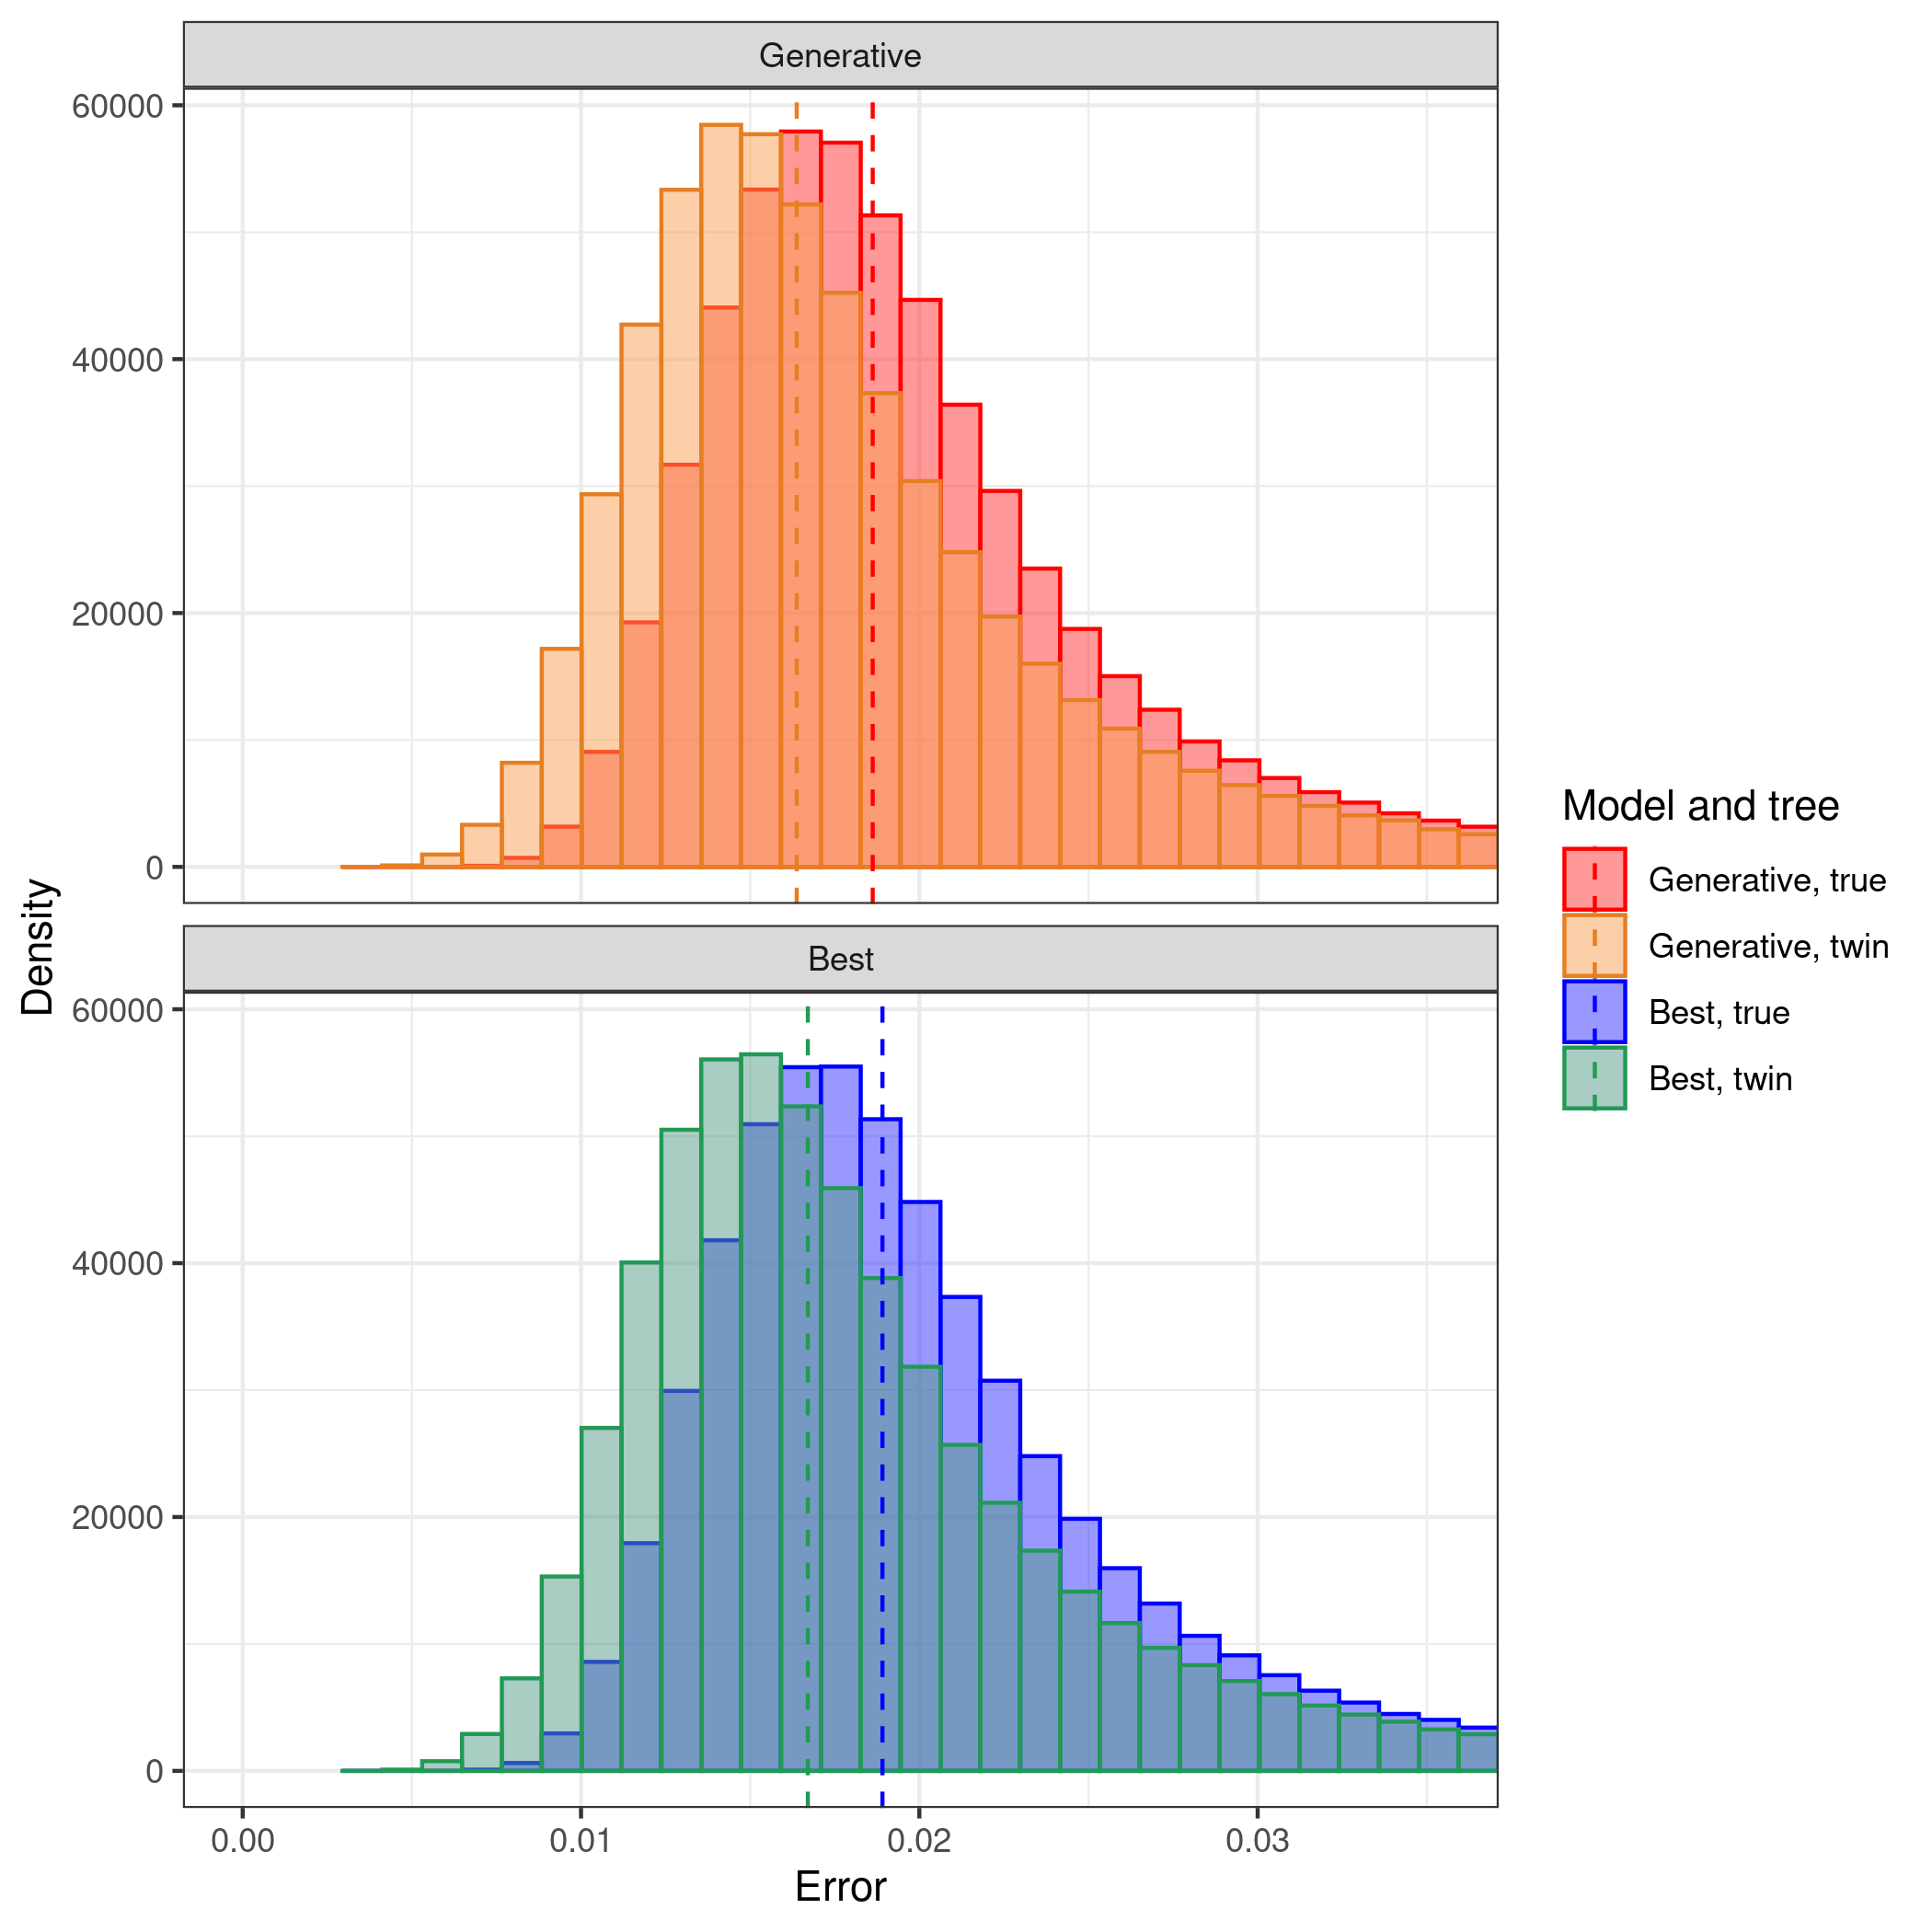
\includegraphics[width=\textwidth]{pirouette_example_41/errors.png}
  \caption{32 taxa, 7 hours}
\end{figure}

\begin{figure}[H]
  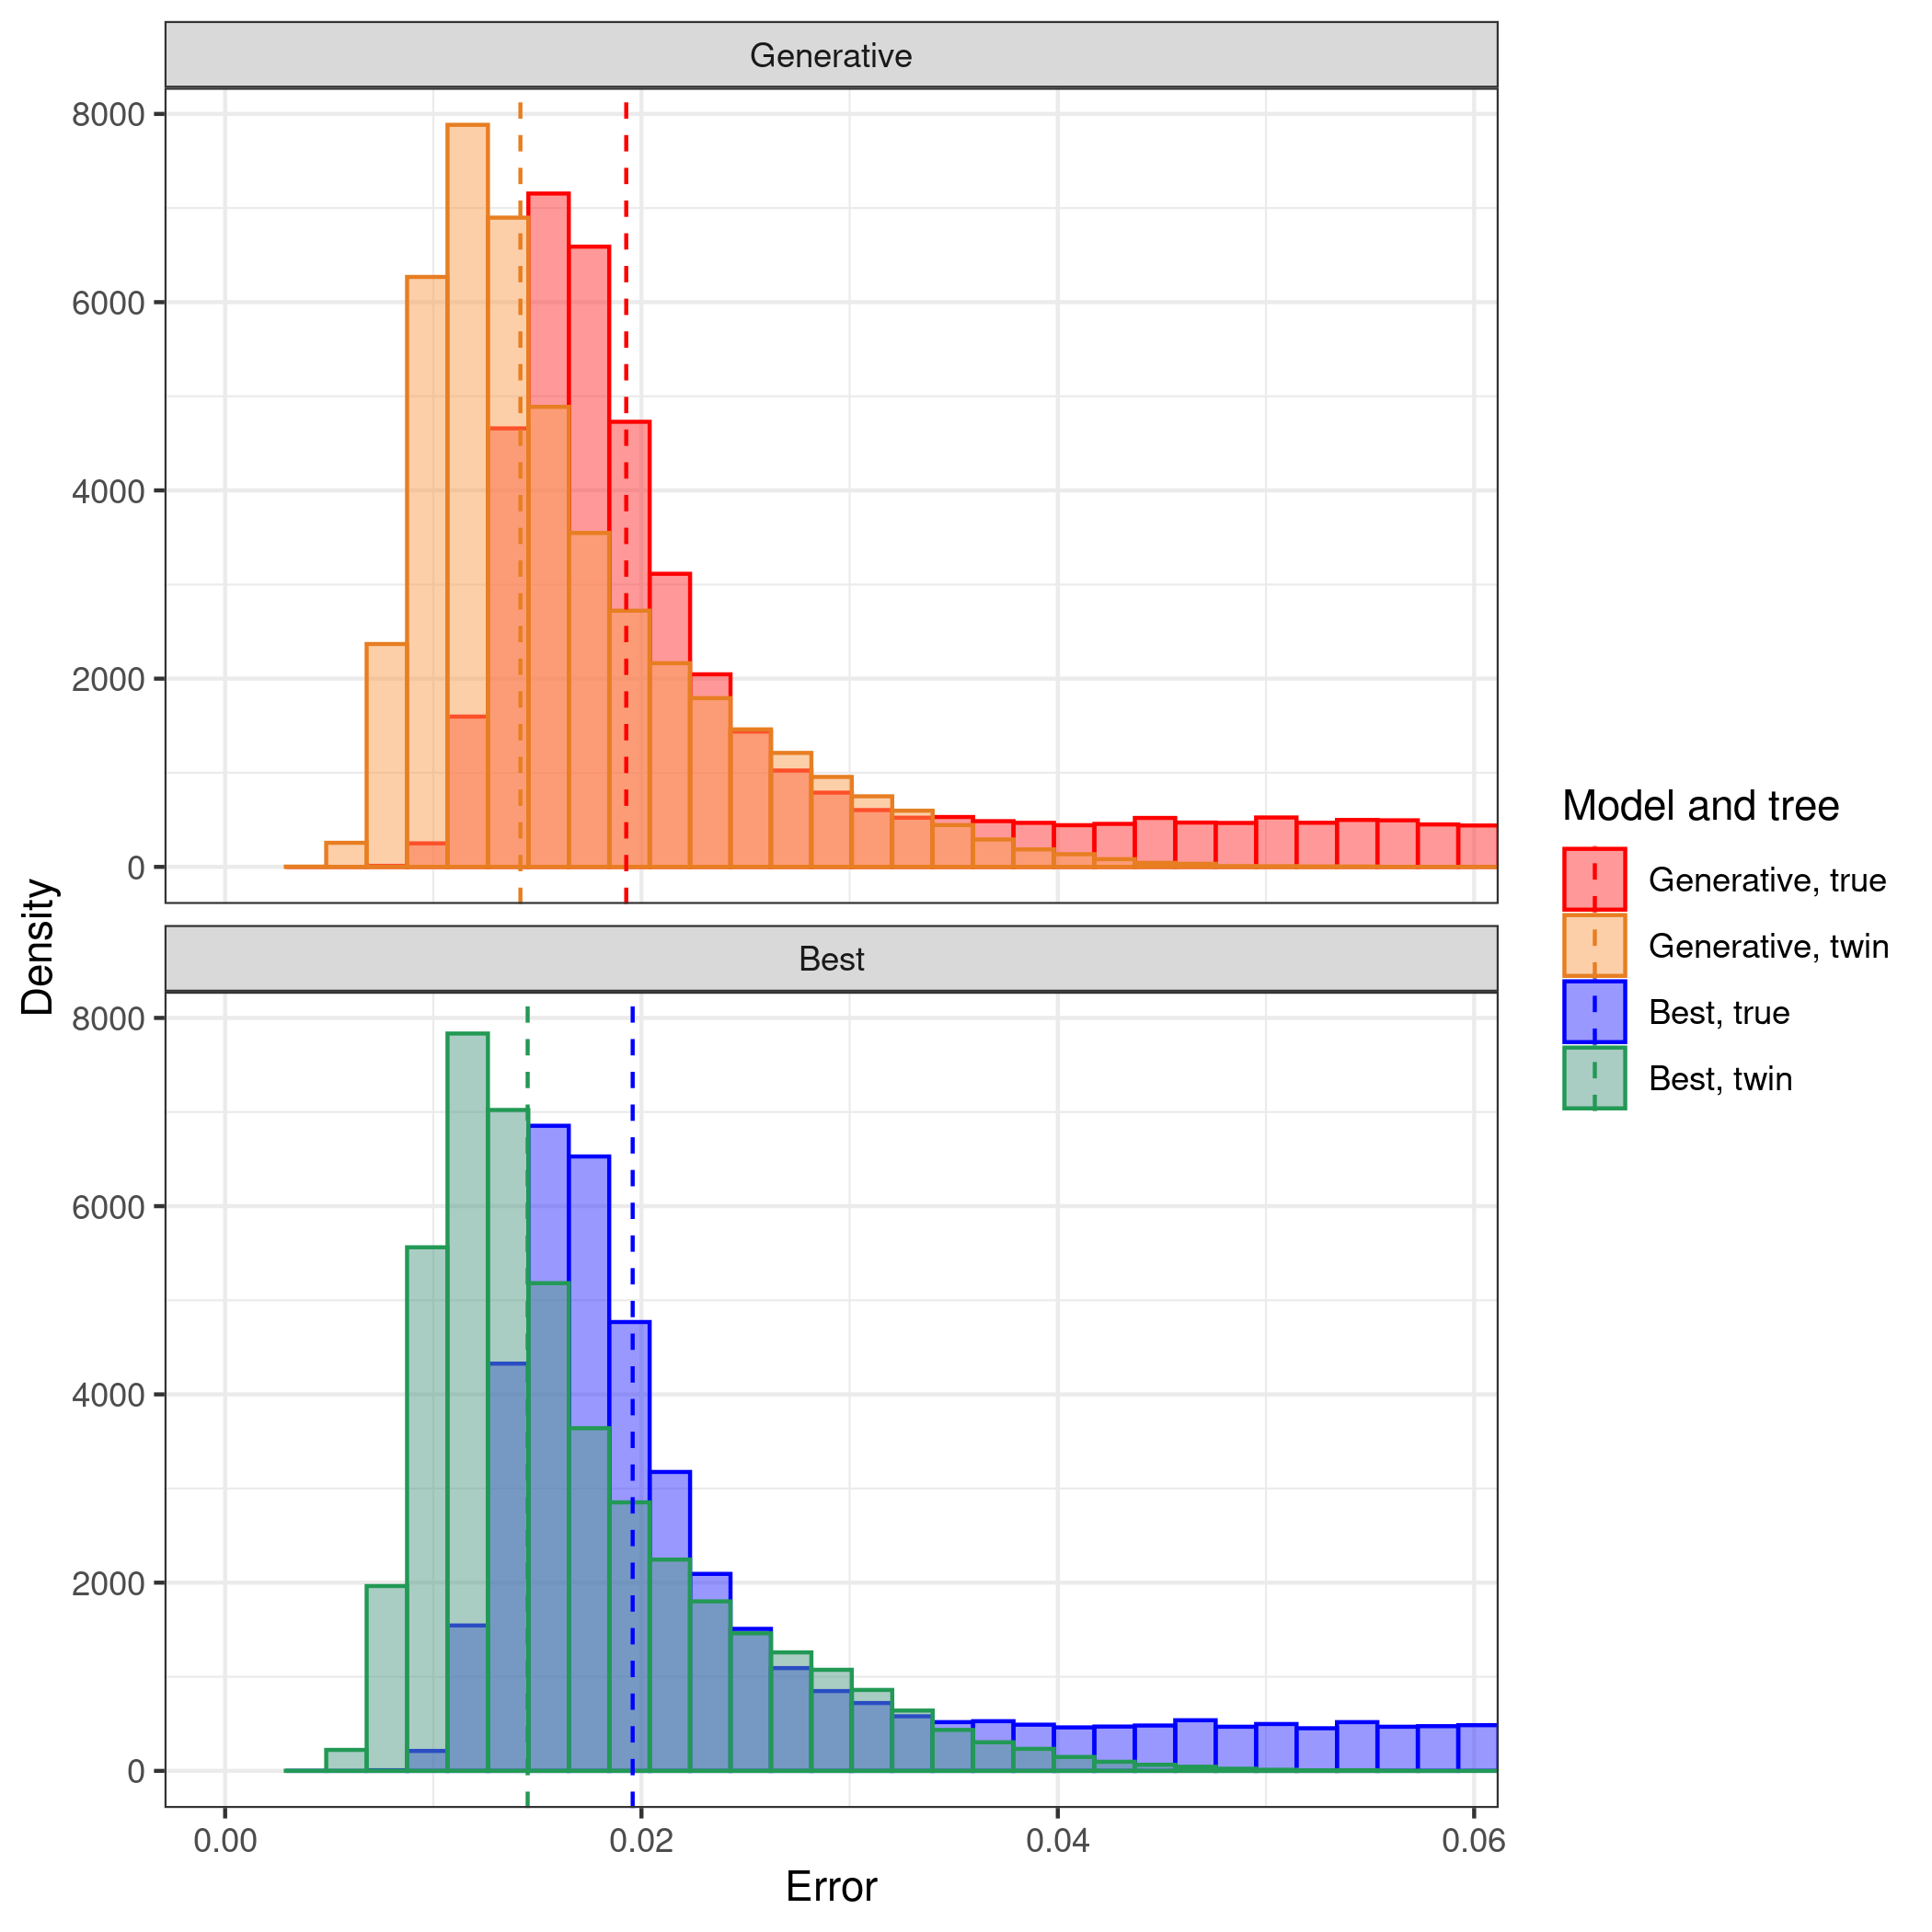
\includegraphics[width=\textwidth]{pirouette_example_42/errors.png}
  \caption{40 taxa, 8 hours}
\end{figure}

%%%%%%%%%%%%%%%%%%%%%%%%%%%%%%%%%%%%%%%%%%%%%%%%%%%%%%%%%%%%%%%%%%%%%%%%%%%%%%%%
\subsection{The effect of DNA sequence length}
\label{subsec:n_nucleotides}
%%%%%%%%%%%%%%%%%%%%%%%%%%%%%%%%%%%%%%%%%%%%%%%%%%%%%%%%%%%%%%%%%%%%%%%%%%%%%%%%

The main example uses a DNA alignment length of 1000 nucleotides.
Here, we show the same results as the main example,
except for a varying DNA alignment sequence length.

The code used in this part of the article can be found at 
\url{https://github.com/richelbilderbeek/pirouette_example_19} (500 nucleotides),
\url{https://github.com/richelbilderbeek/pirouette_example_28} (1000 nucleotides, main example),
and \url{https://github.com/richelbilderbeek/pirouette_example_34} (2000 nucleotides).

\begin{figure}[H]
  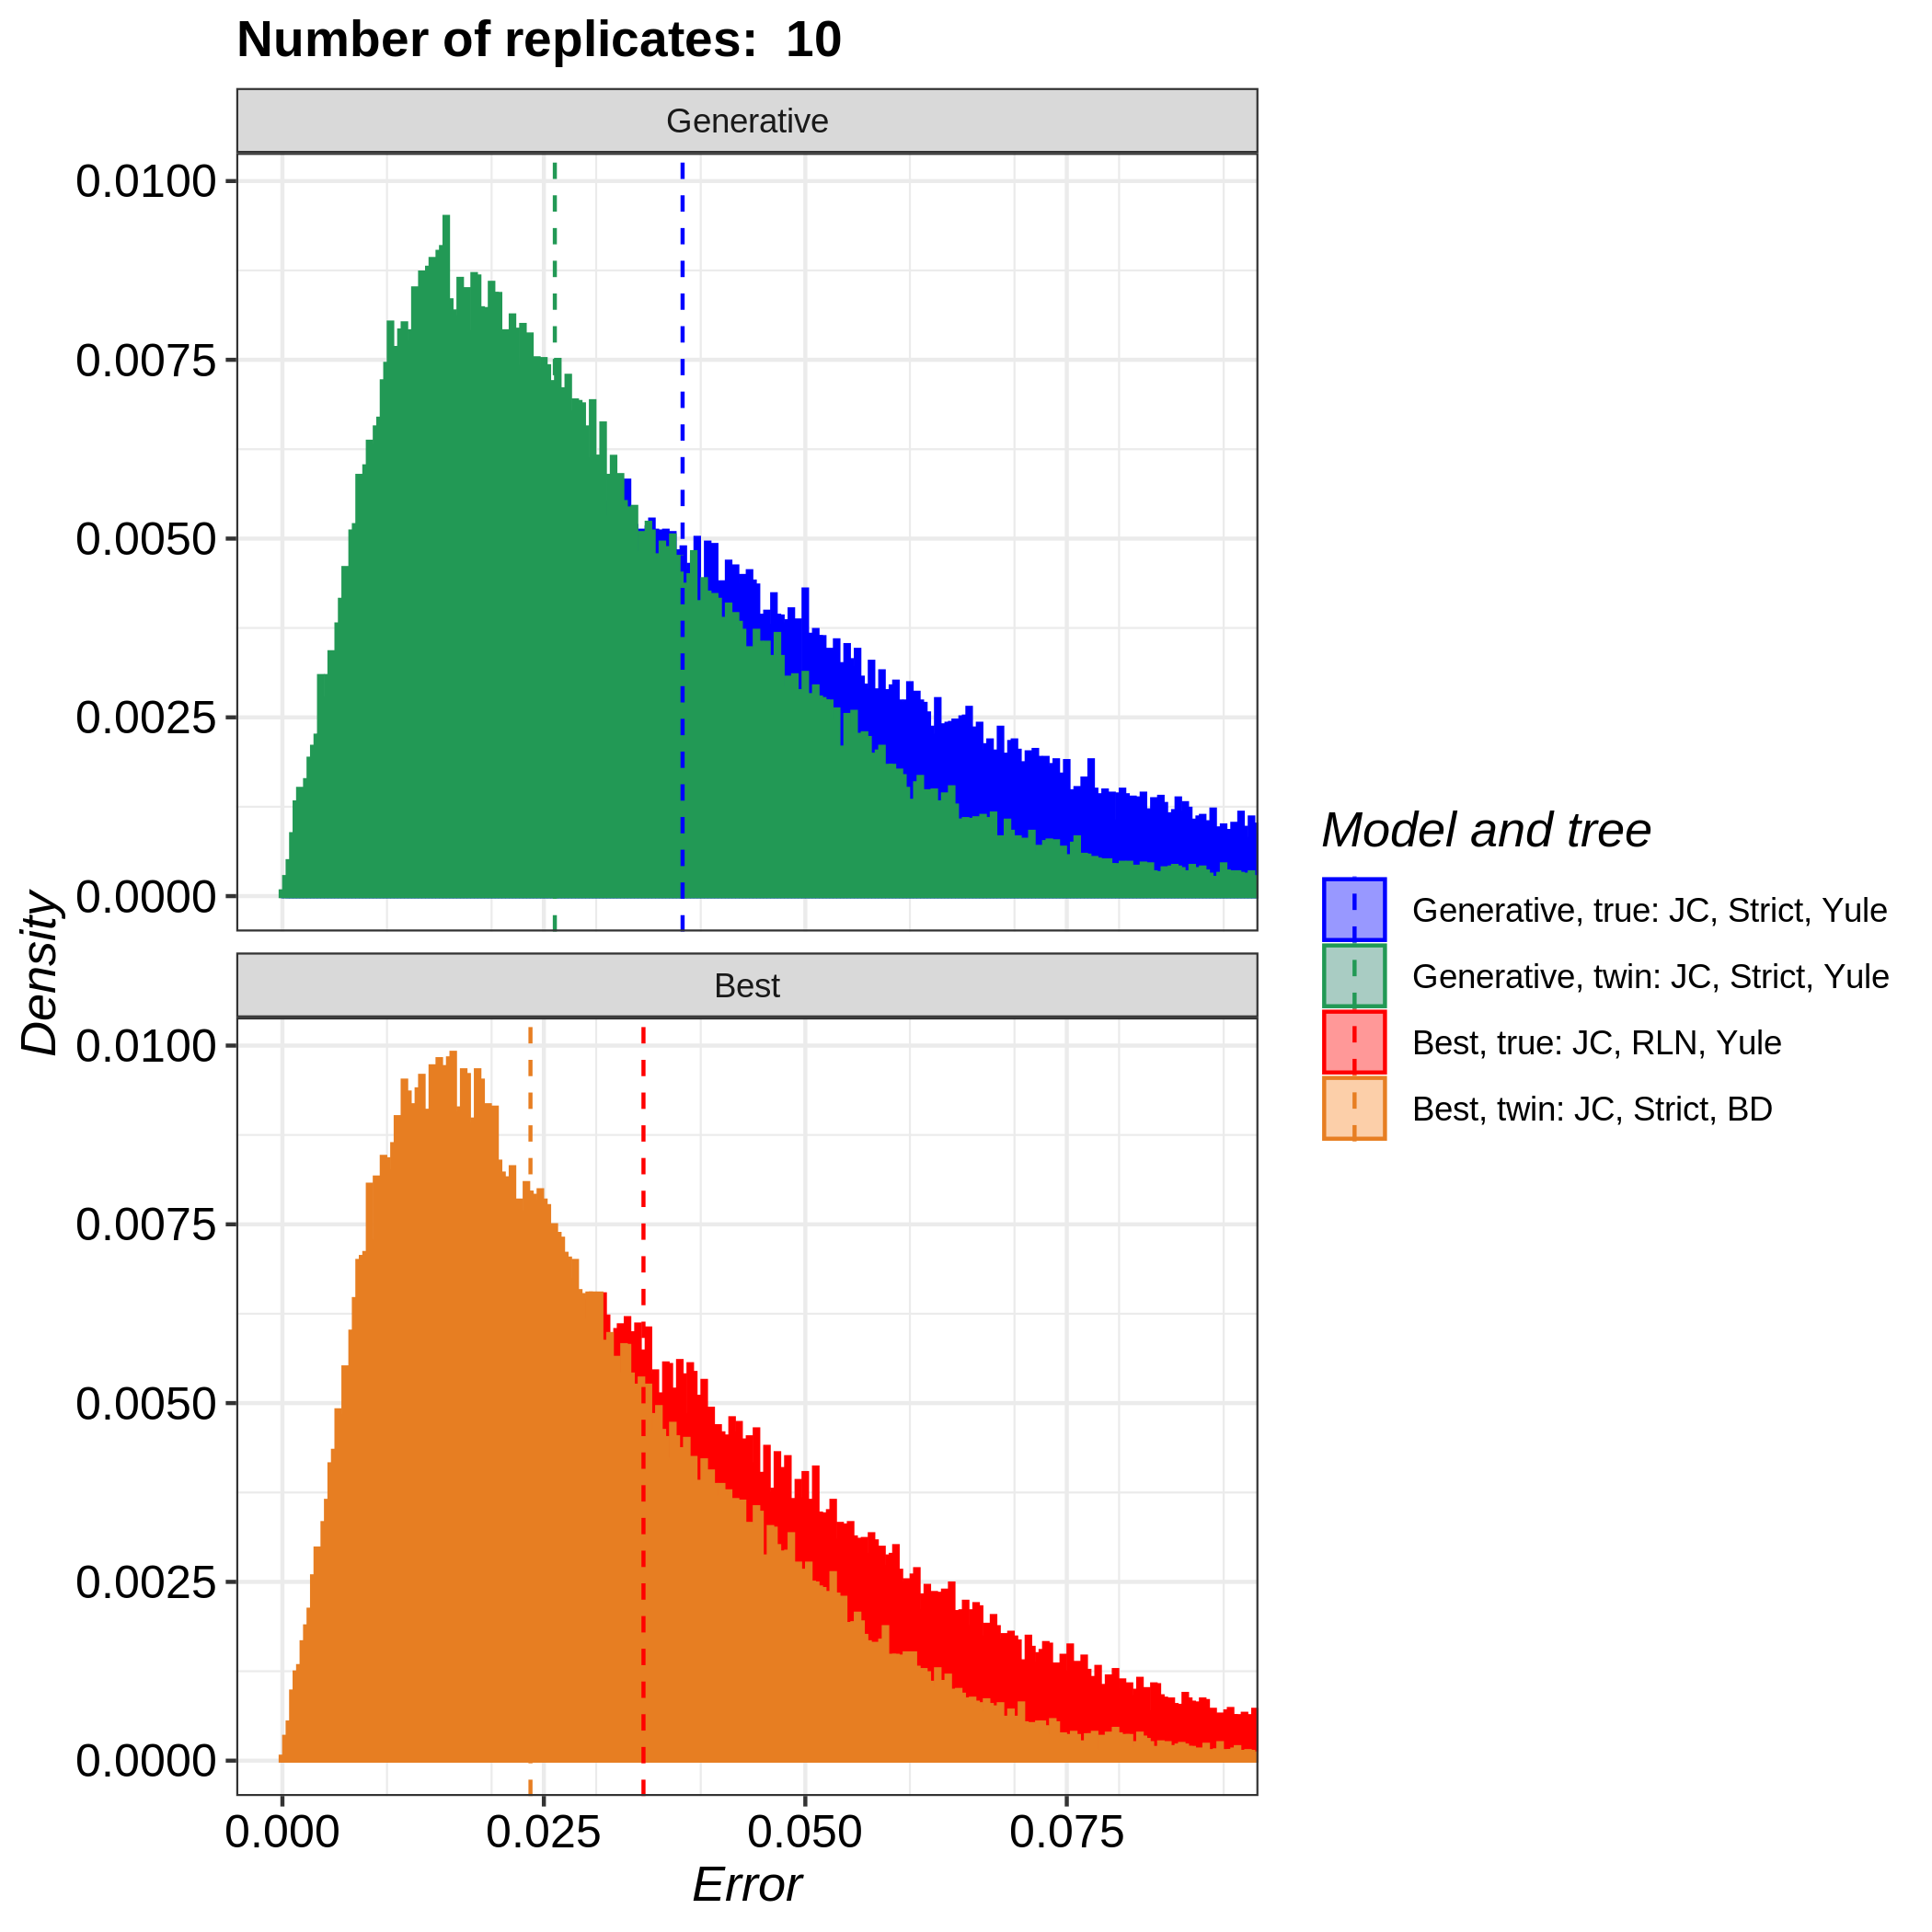
\includegraphics[width=\textwidth]{pirouette_example_19/errors.png}
  \caption{500 nucleotides, 12 hours}
\end{figure}

\begin{figure}[H]
  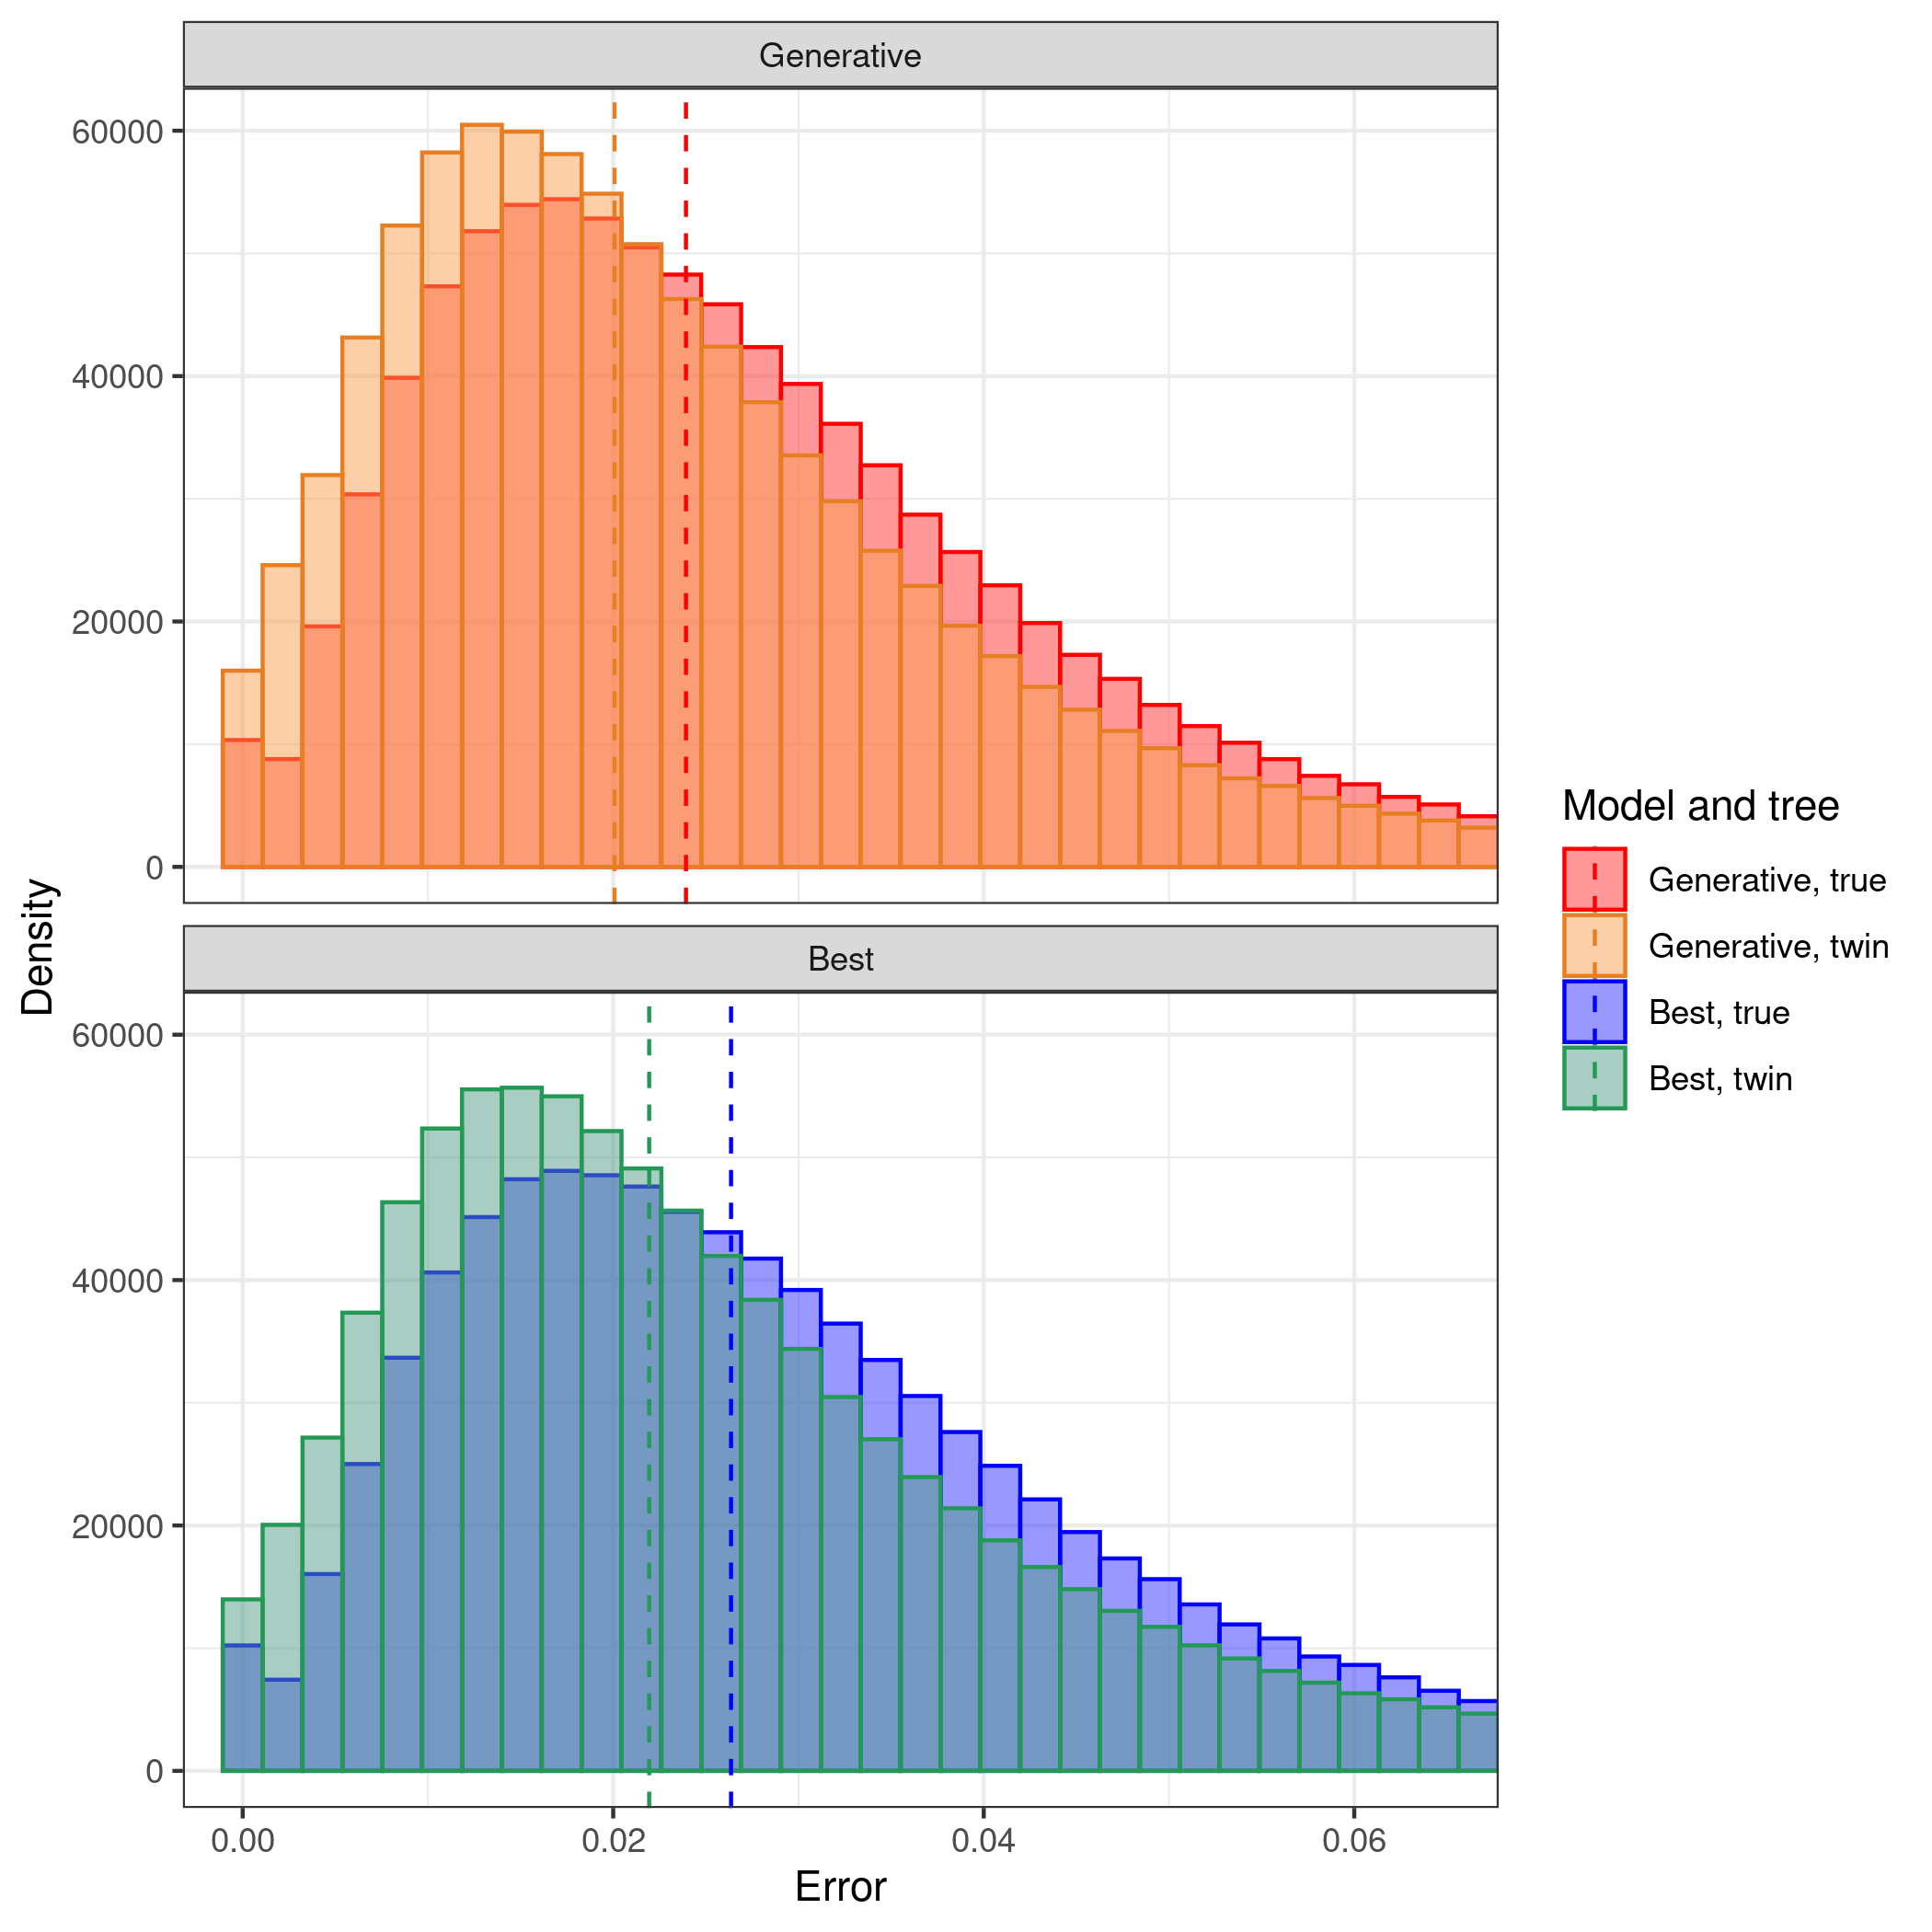
\includegraphics[width=\textwidth]{pirouette_example_28/errors.png}
  \caption{1000 nucleotides, 16 hours (main example)}
\end{figure}

\begin{figure}[H]
  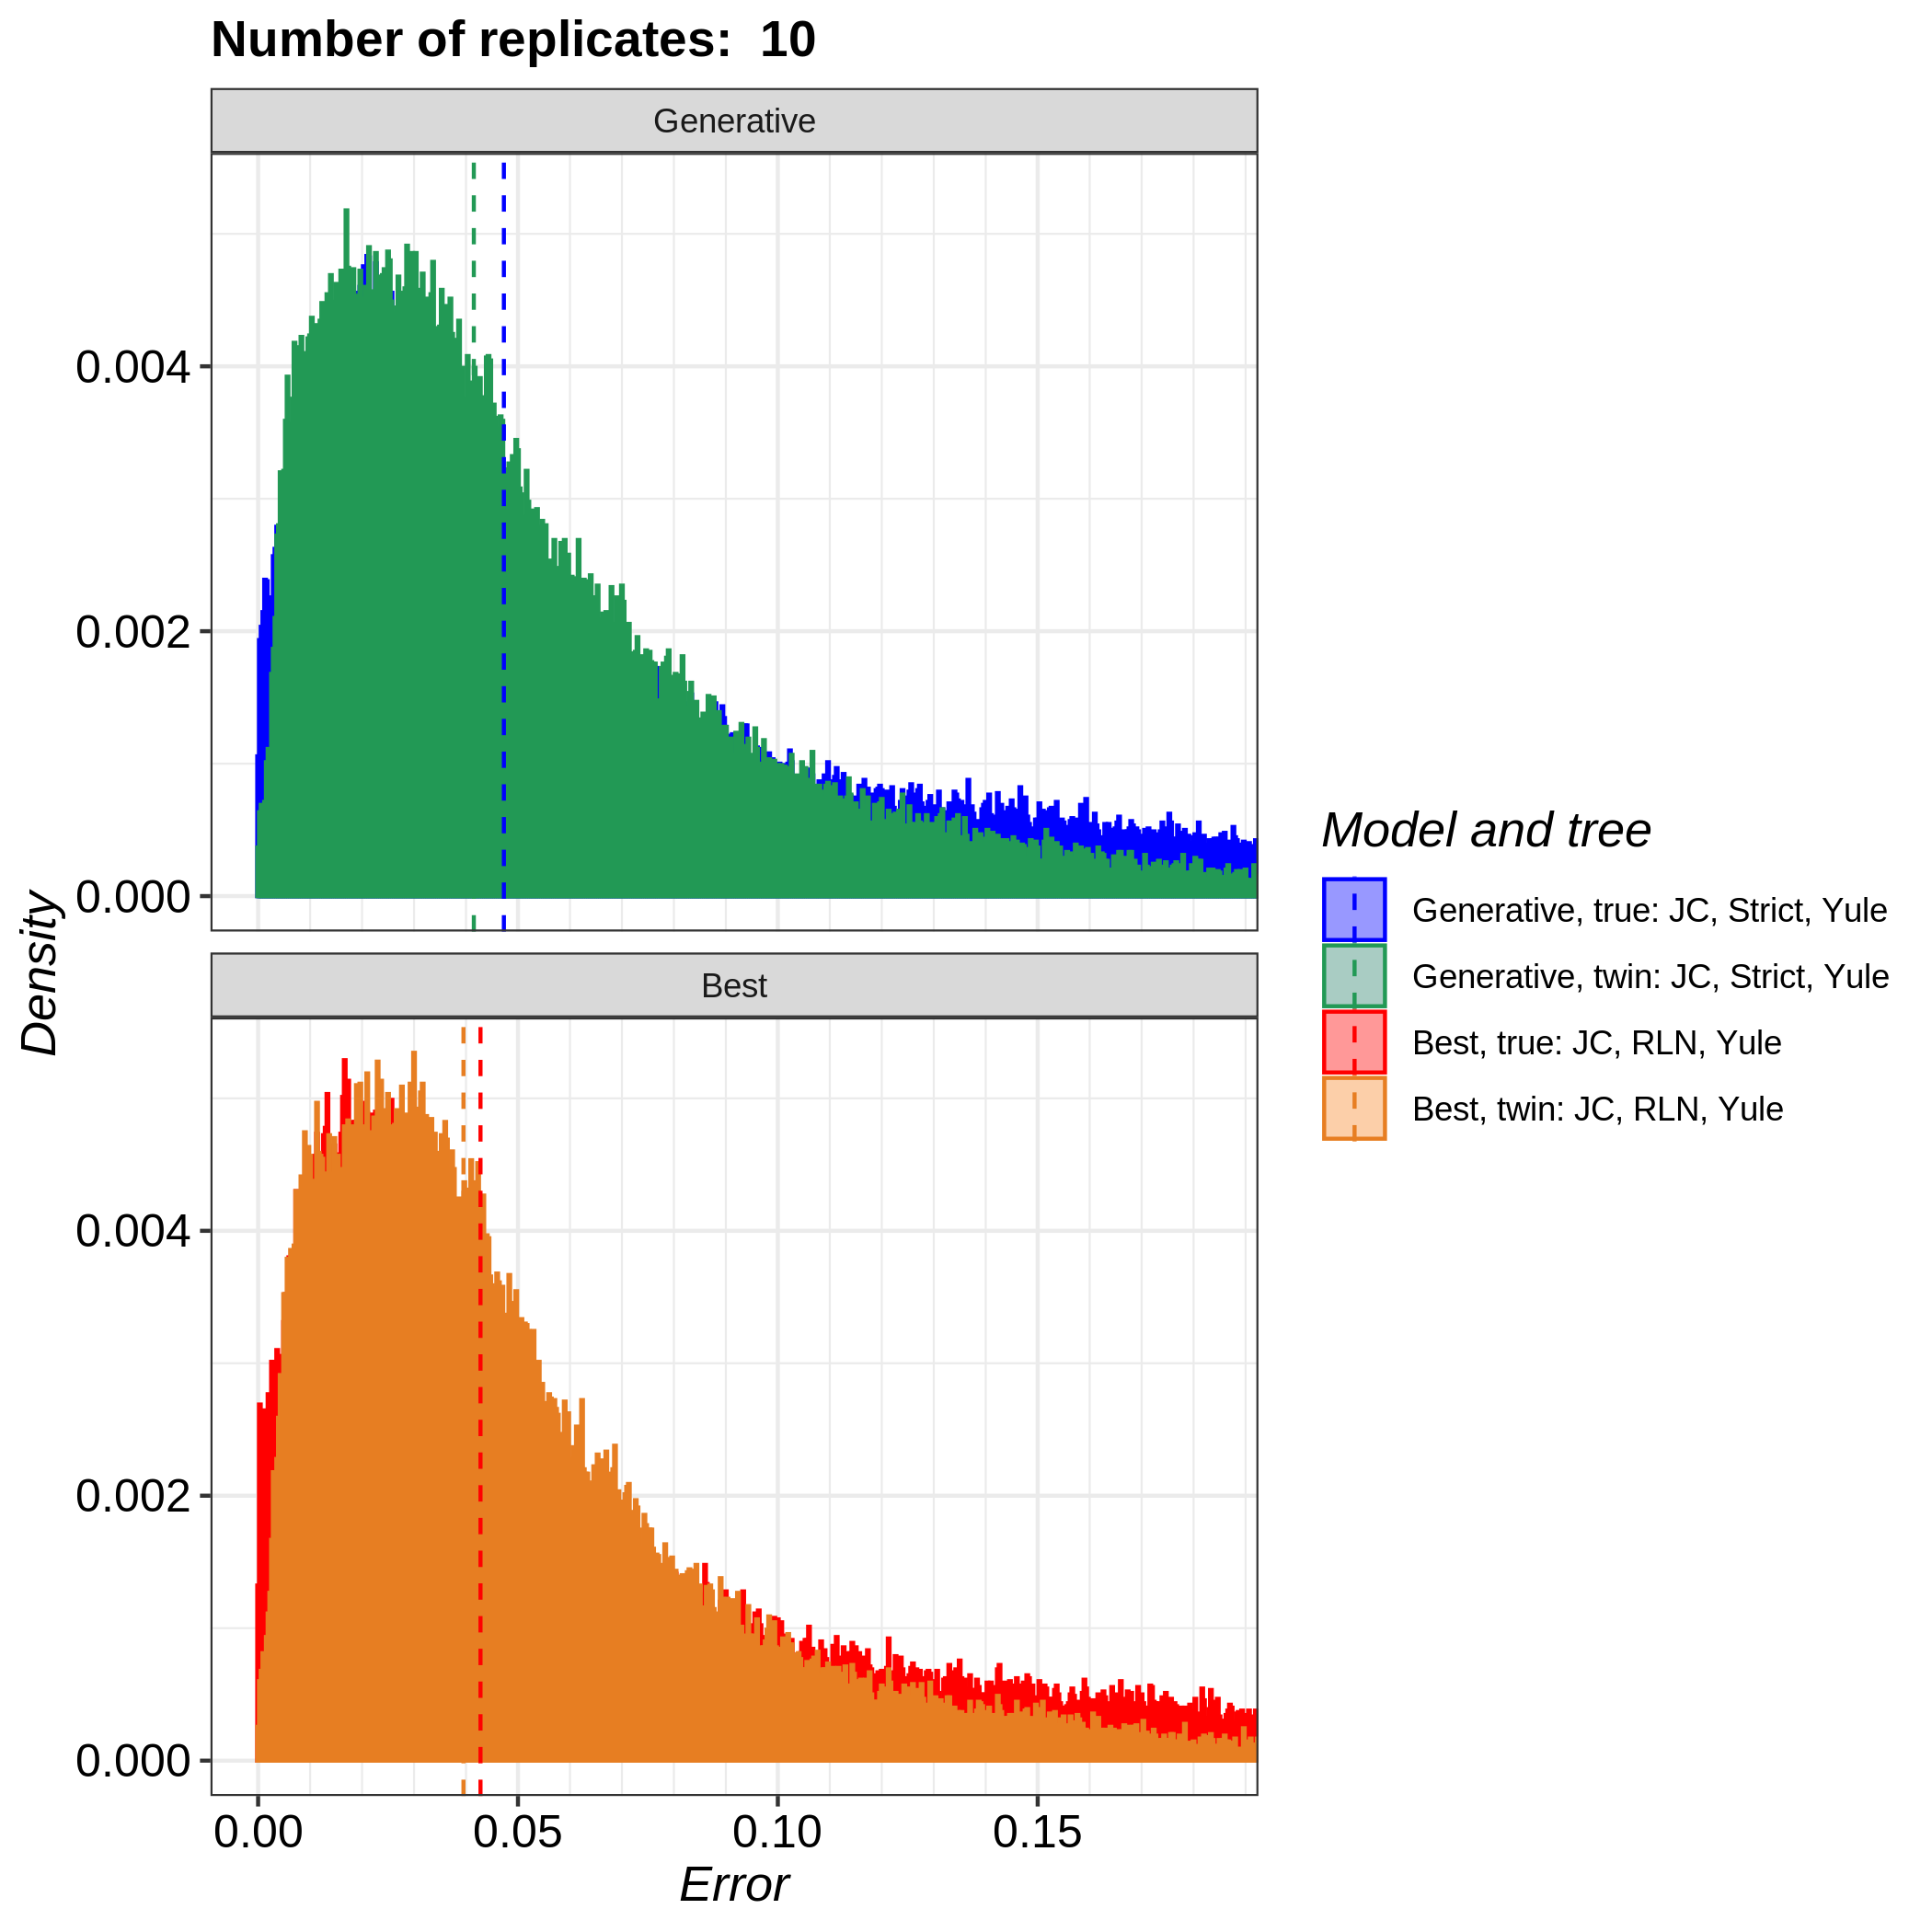
\includegraphics[width=\textwidth]{pirouette_example_34/errors.png}
  \caption{2000 nucleotides, 11 hours}
\end{figure}


%%%%%%%%%%%%%%%%%%%%%%%%%%%%%%%%%%%%%%%%%%%%%%%%%%%%%%%%%%%%%%%%%%%%%%%%%%%%%%%%
\subsection{The effect of non-clock like models}
\label{subsec:non_clock}
%%%%%%%%%%%%%%%%%%%%%%%%%%%%%%%%%%%%%%%%%%%%%%%%%%%%%%%%%%%%%%%%%%%%%%%%%%%%%%%%

The main example generates an alignment using a strict clock model (that is,
all species have an equal mutation rate).
One may wonder, how well the inference will be for a different non-clock like
model.
Here, we show the same results as the main example,
except that instead of generating the alignment with a strict clock
model, we use an unlinked node substitution model (by Thijs Janzen,
unpublished, code available at \url{https://github.com/thijsjanzen/nodeSub}),
with a branch mutation rate of $0.1$ and a node mutation rate of $0.1$.

The code used in this part of the article can be found at 
\url{https://github.com/richelbilderbeek/pirouette_example_27}.

\begin{figure}[H]
  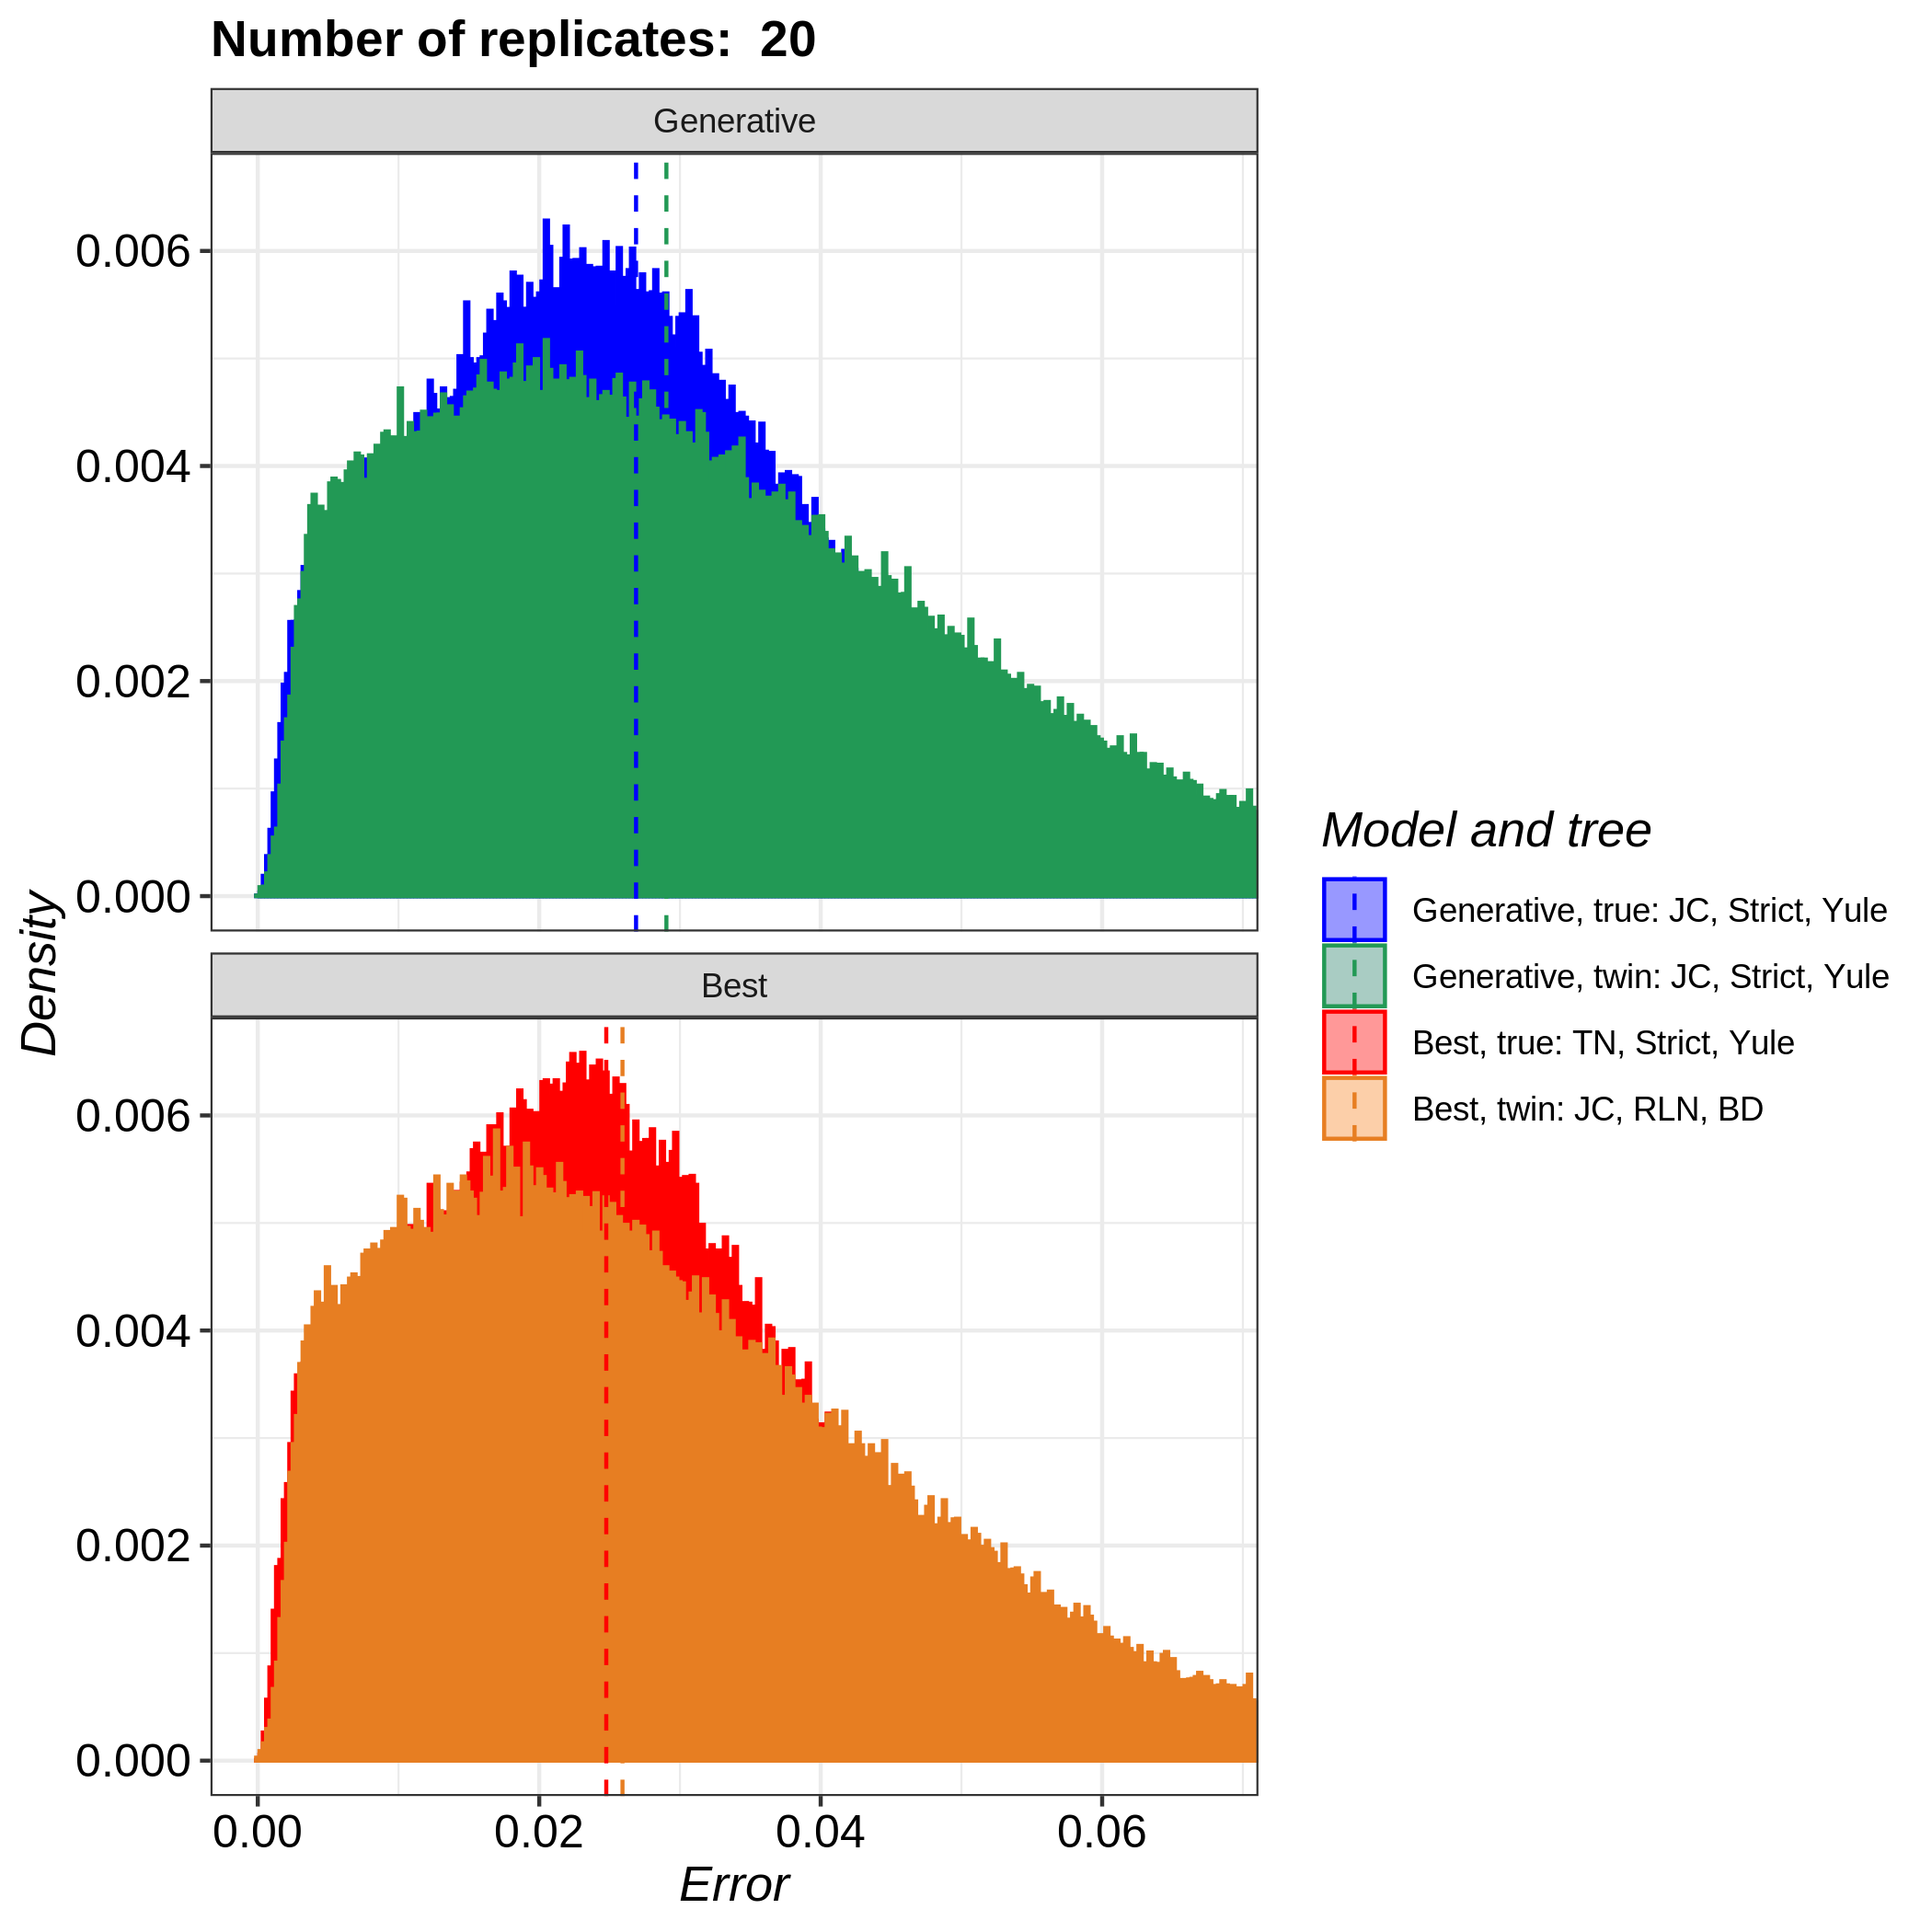
\includegraphics[width=\textwidth]{pirouette_example_27/errors.png}
  \caption{An unlinked node substitution model, 20 replicates, 8 hours}
\end{figure}

%%%%%%%%%%%%%%%%%%%%%%%%%%%%%%%%%%%%%%%%%%%%%%%%%%%%%%%%%%%%%%%%%%%%%%%%%%%%%%%%
\subsection{The effect of assuming a Yule tree prior on a Yule tree}
\label{subsec:simplest_correct_parameterization}
%%%%%%%%%%%%%%%%%%%%%%%%%%%%%%%%%%%%%%%%%%%%%%%%%%%%%%%%%%%%%%%%%%%%%%%%%%%%%%%%

The main example uses a tree generated by a non-standard tree model.
Here, we show the same results, with the only difference that
the tree used is generated by simplest tree model (the Yule model),
which we also assume as the (correct) tree prior.
This example thus shows a parameterization at the correct level for the
simplest case possible.

The code used in this part of the article can be found at 
\url{https://github.com/richelbilderbeek/pirouette_example_22}.

\begin{figure}[H]
  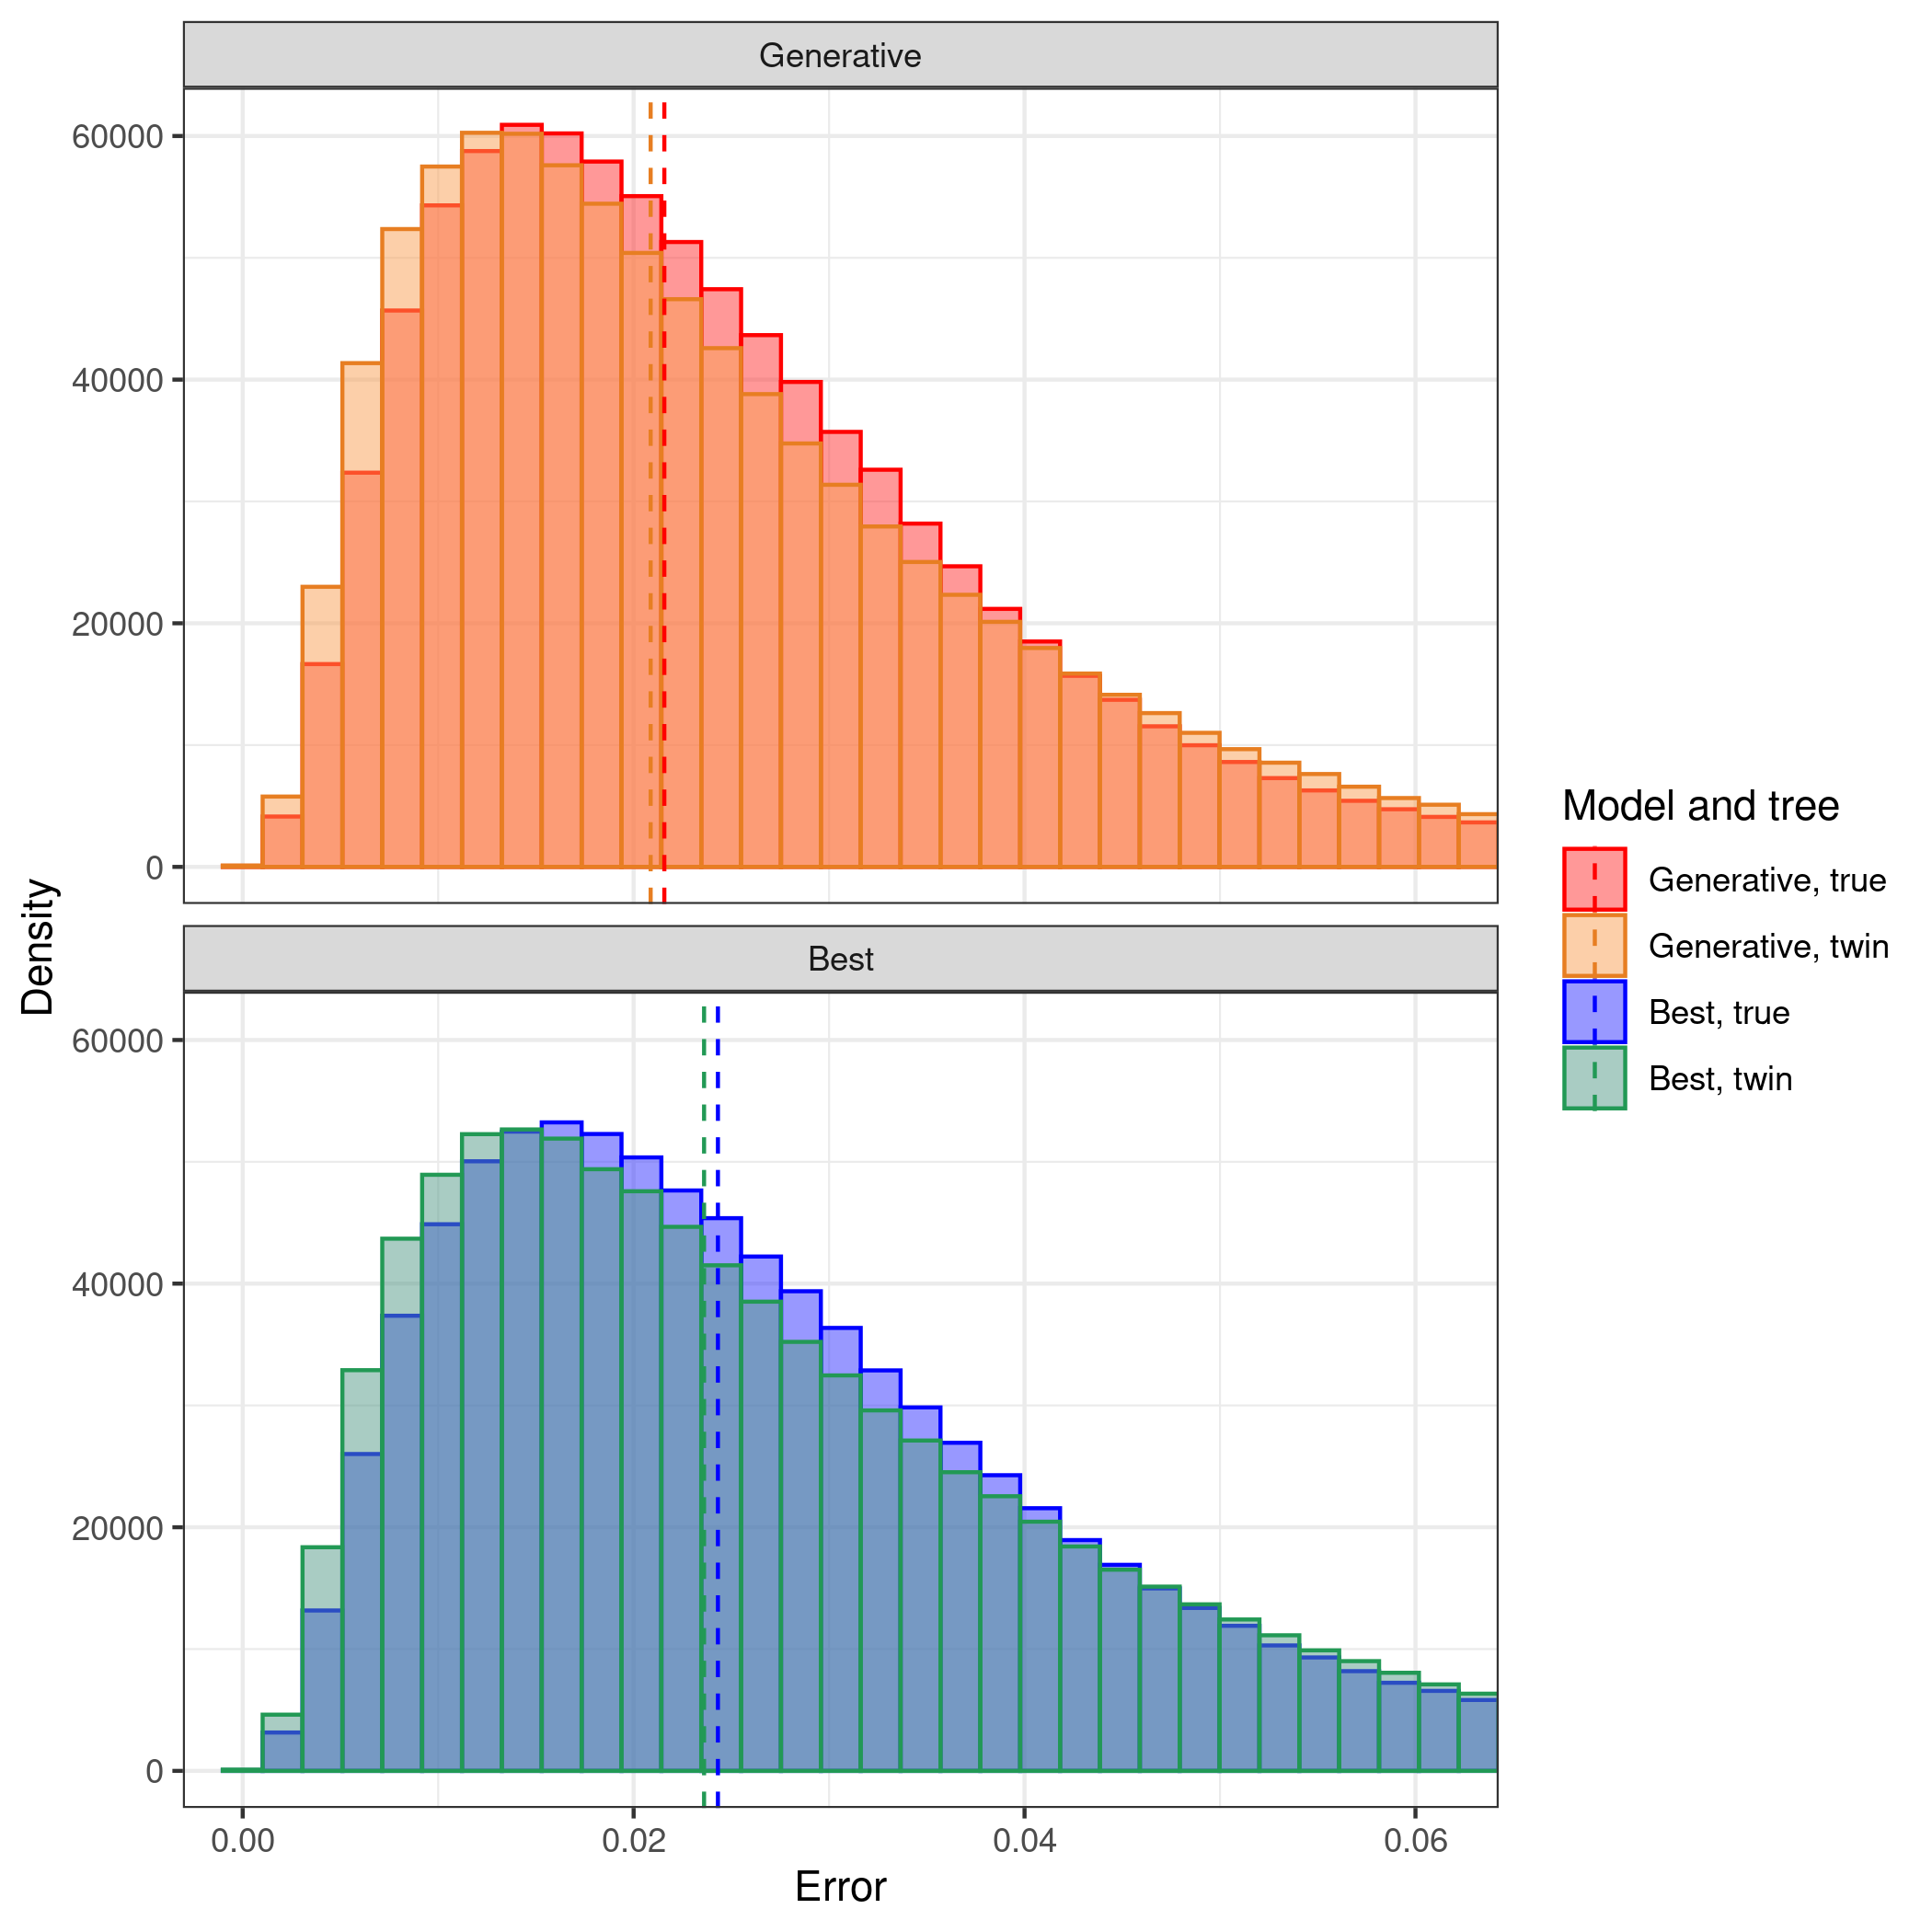
\includegraphics[width=\textwidth]{pirouette_example_22/errors.png}
  \caption{Assuming a Yule tree prior on a Yule tree, 9 hours}
\end{figure}

%%%%%%%%%%%%%%%%%%%%%%%%%%%%%%%%%%%%%%%%%%%%%%%%%%%%%%%%%%%%%%%%%%%%%%%%%%%%%%%%
\subsection{The effect of assuming a Yule tree prior on a BD tree}
\label{subsec:under_parameterization}
%%%%%%%%%%%%%%%%%%%%%%%%%%%%%%%%%%%%%%%%%%%%%%%%%%%%%%%%%%%%%%%%%%%%%%%%%%%%%%%%

The main example uses a tree generated by a non-standard tree model.

Here, we show the same results, with the difference that
the tree used is generated by a birth-death (BD) tree model,
where we assume it is generated by a Yule (or pure-birth) model.
This example thus shows the effect of underparameterization.

The code used in this part of the article can be found at 
\url{https://github.com/richelbilderbeek/pirouette_example_26}.

\begin{figure}[H]
  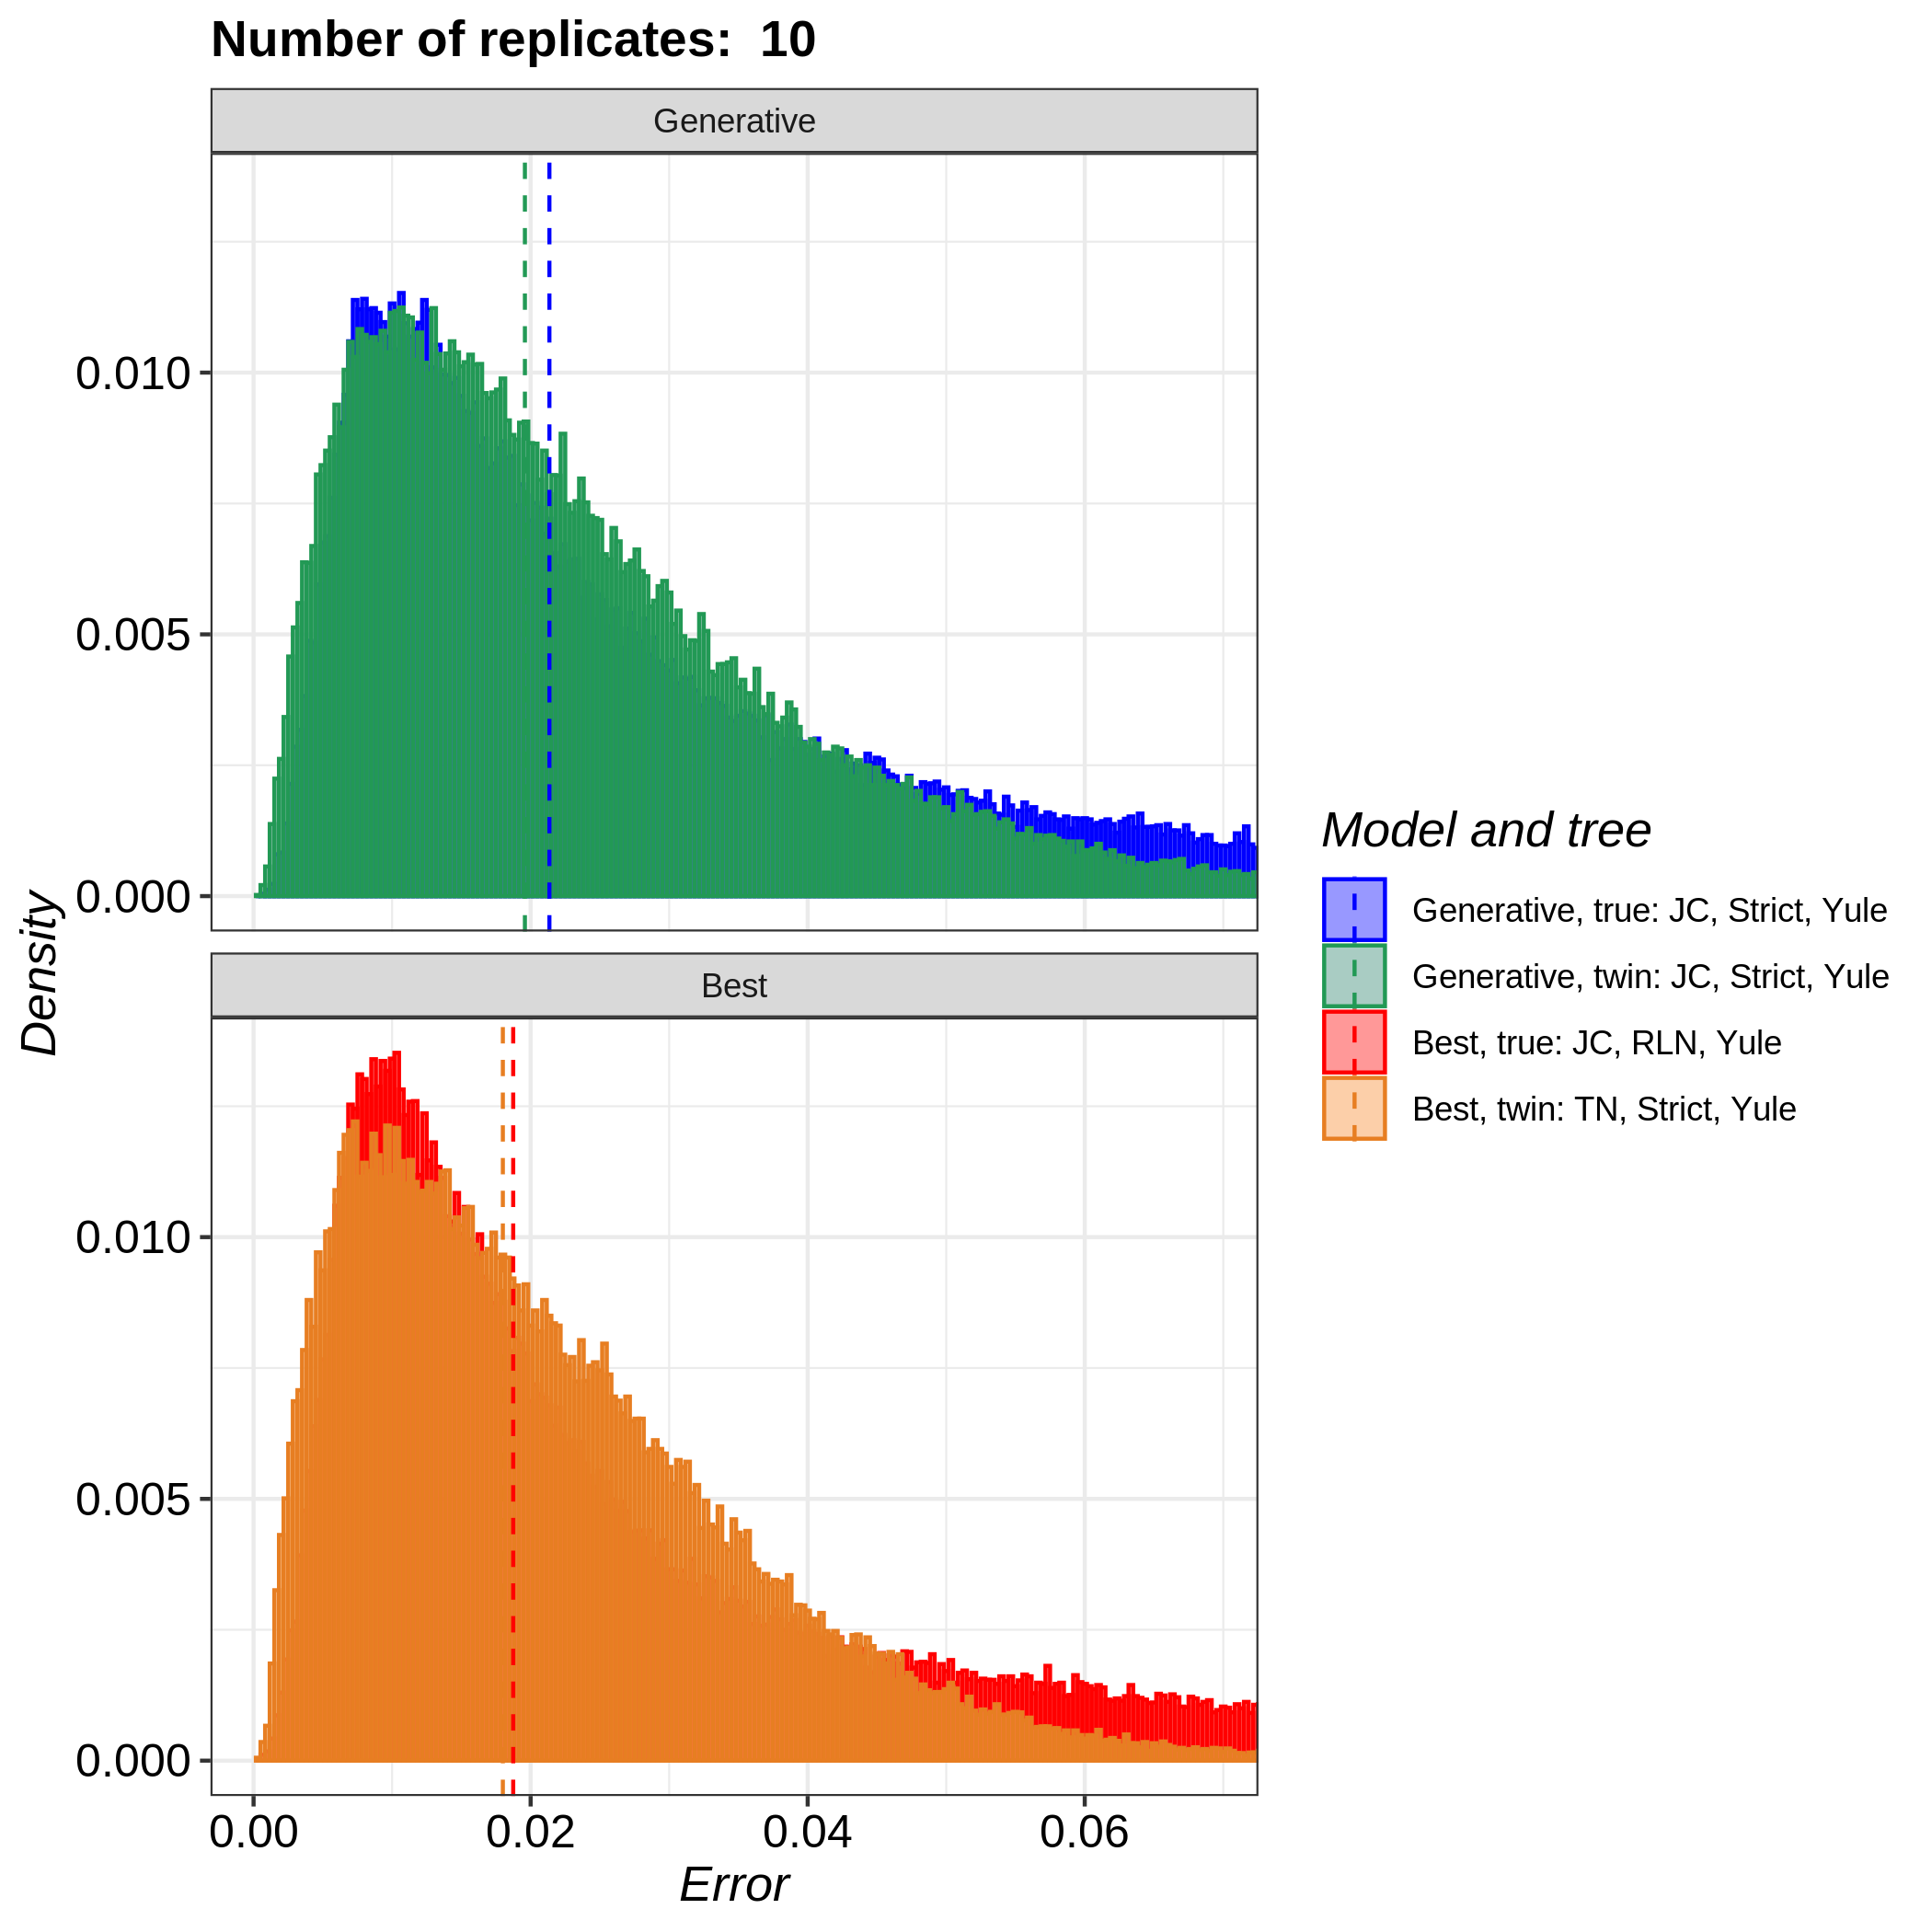
\includegraphics[width=\textwidth]{pirouette_example_26/errors.png}
  \caption{Assuming a Yule tree prior on a BD tree, 9 hours}
\end{figure}

%%%%%%%%%%%%%%%%%%%%%%%%%%%%%%%%%%%%%%%%%%%%%%%%%%%%%%%%%%%%%%%%%%%%%%%%%%%%%%%%
\subsection{The effect of differently common diversity-dependent trees}
\label{subsec:better_label_needed}
%%%%%%%%%%%%%%%%%%%%%%%%%%%%%%%%%%%%%%%%%%%%%%%%%%%%%%%%%%%%%%%%%%%%%%%%%%%%%%%%

Here we show the results of a \verb;pirouette; run on a dataset 
of 2 trees simulated under a diversity-dependent process. 
All the trees are simulated using the DDD package (\cite{DDD}). 
Our goal is to show how trees simulated by a process that is 
sensibly different from a standard tree prior will result in a 
significant divergence between true and twin distribution. 
To do so we set the simulation parameters (in this case: 
absolute speciation rate $\lambda_0 = 1.6$, 
extinction rate $\mu = 0.2$ and carrying capacity $K = 20$) 
in order to express clear characteristics of diversity dependence in the 
phylogenies. In fact, for a high speciation rate and a low carrying capacity, 
we expect trees to exhibit high unbalance, compared with trees generated 
by a standard birth-death model. 
We can measure how unbalanced is a tree using the $\gamma$ 
statistics (\cite{pybus2000testing}). For this reason, we choose to 
measure the error made by the inference process using the $\gamma$ error statistics, 
which is currently implemented in \verb;pirouette;.

The code used in this part of the article can be found at 
\url{https://github.com/richelbilderbeek/pirouette_example_23}
and took 120 hours in total.

\begin{figure}[H]
  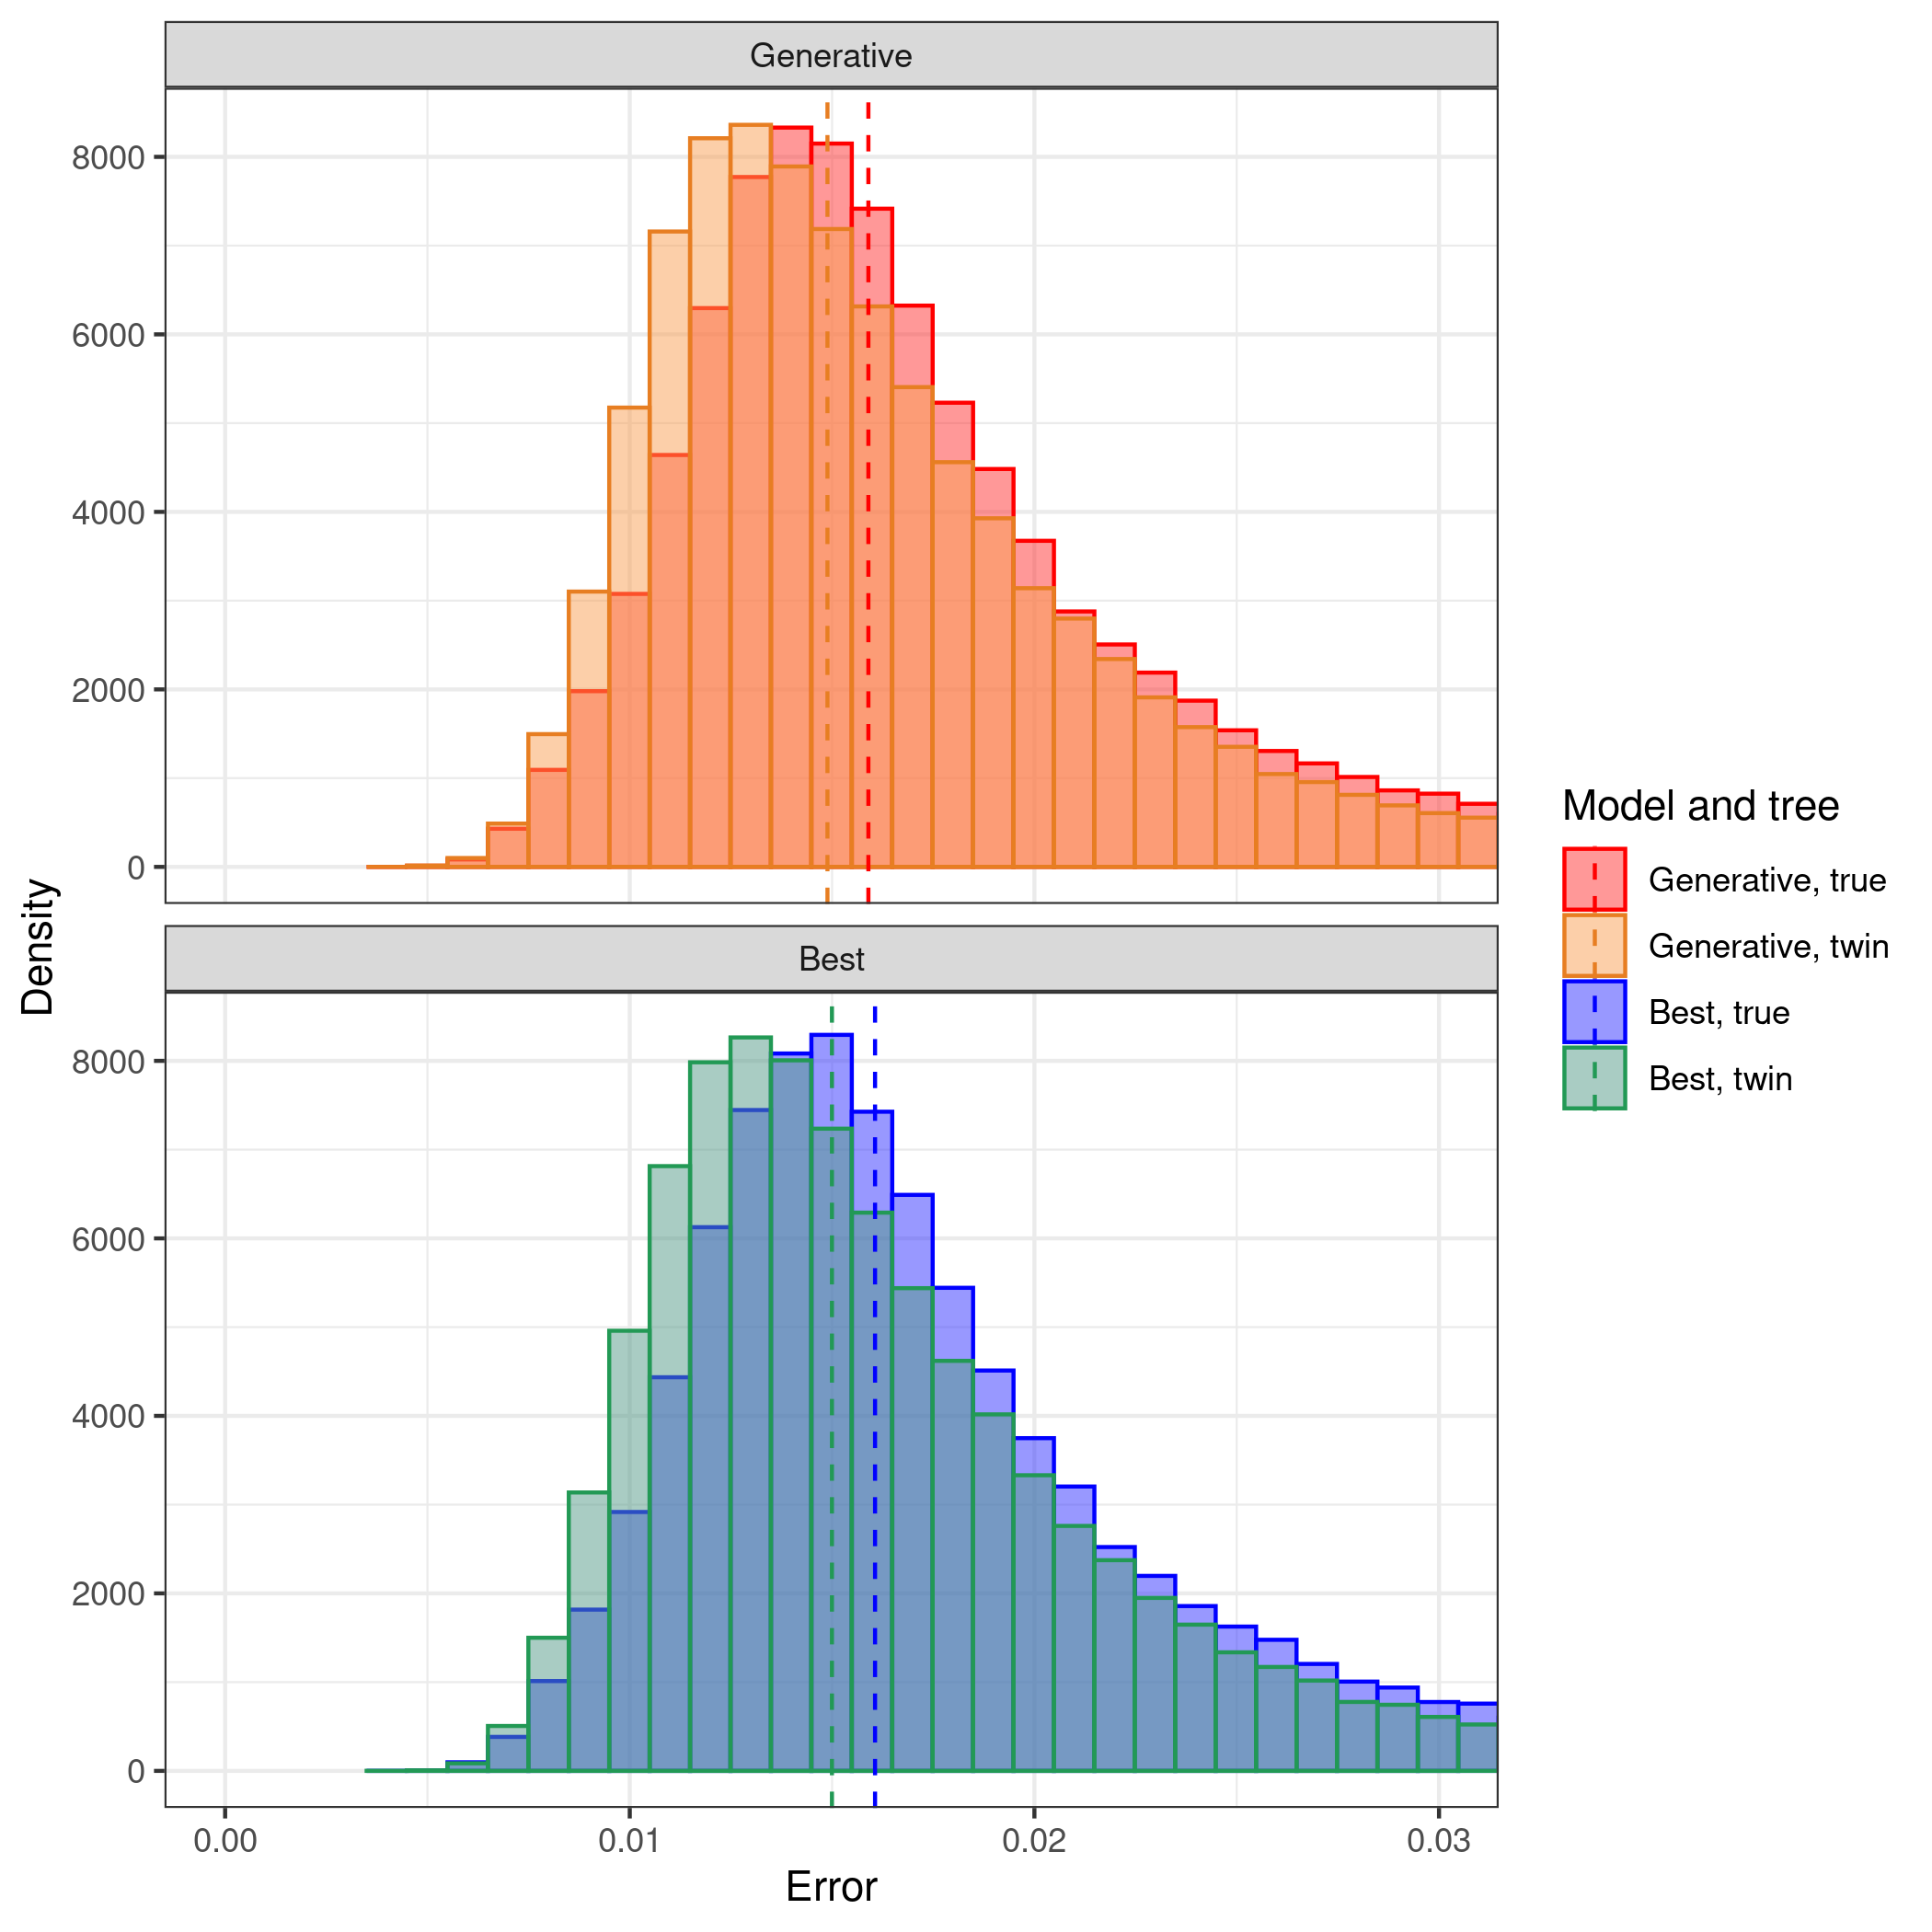
\includegraphics[width=\textwidth]{pirouette_example_23/errors_low.png}
  \caption{Lowest likelihood}
\end{figure}

\begin{figure}[H]
  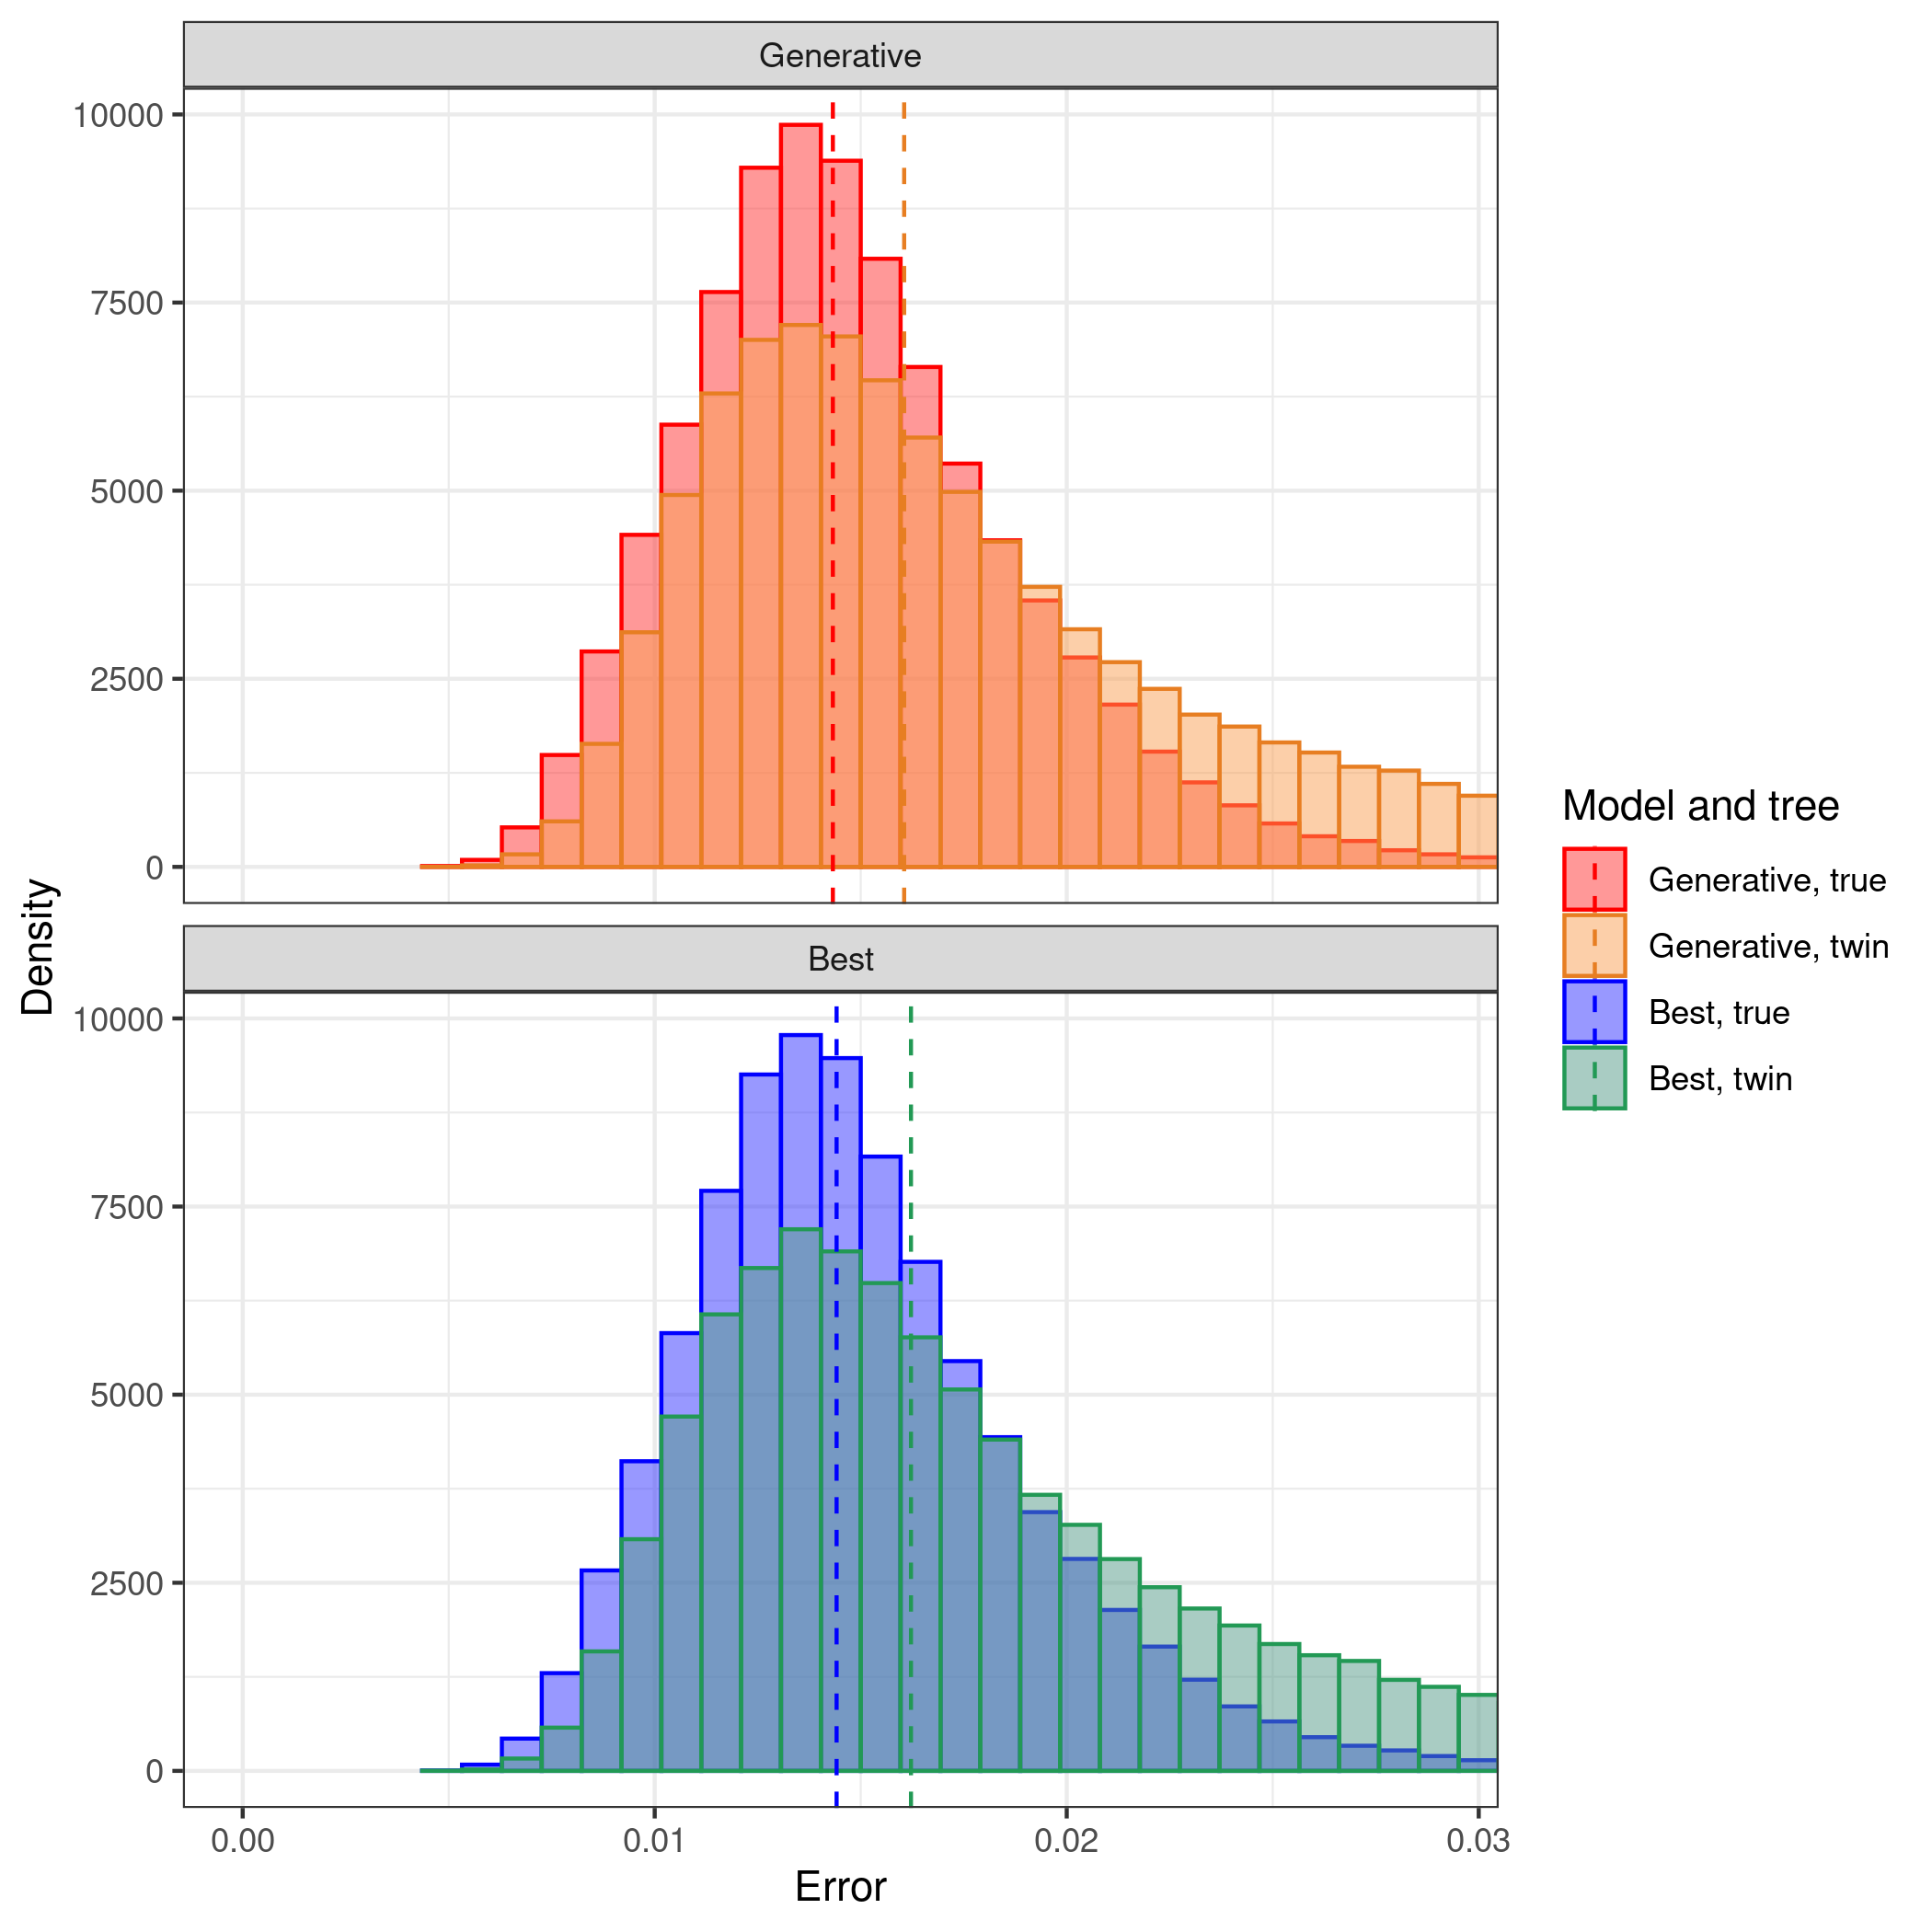
\includegraphics[width=\textwidth]{pirouette_example_23/errors_mid.png}
  \caption{Median likelihood}
\end{figure}

\begin{figure}[H]
  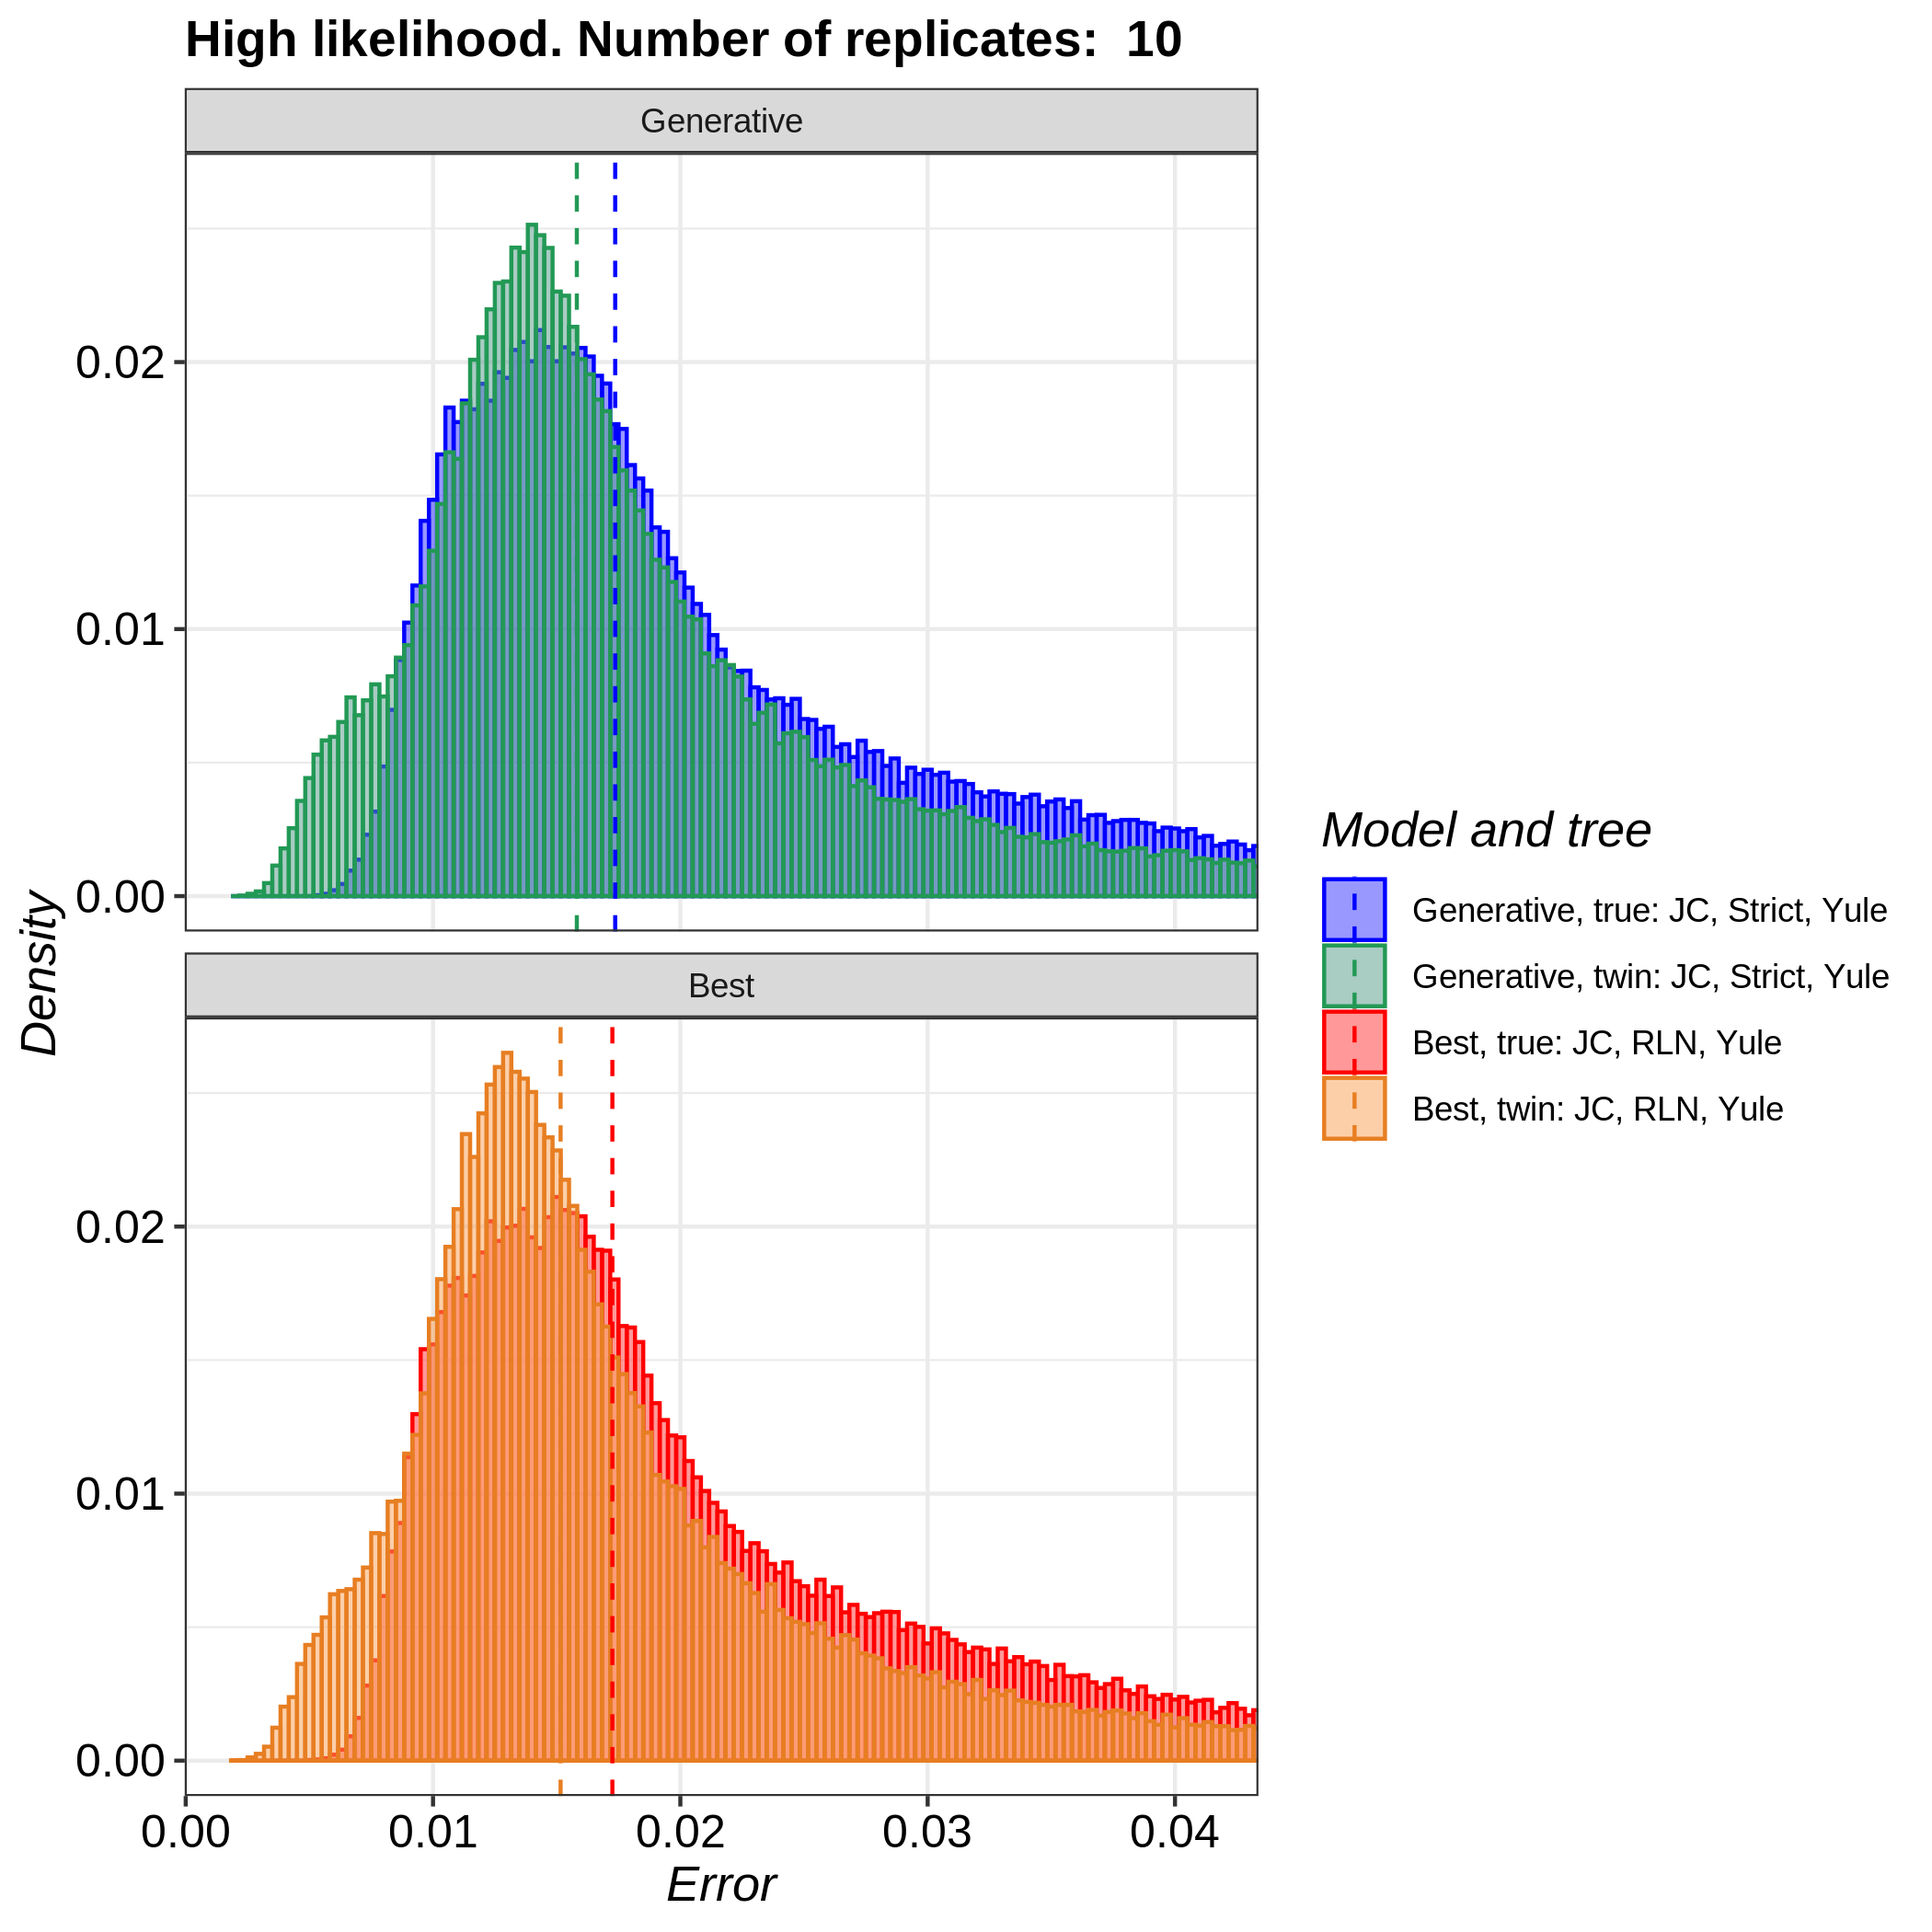
\includegraphics[width=\textwidth]{pirouette_example_23/errors_high.png}
  \caption{Highest likelihood}
\end{figure}

\begin{figure}[H]
  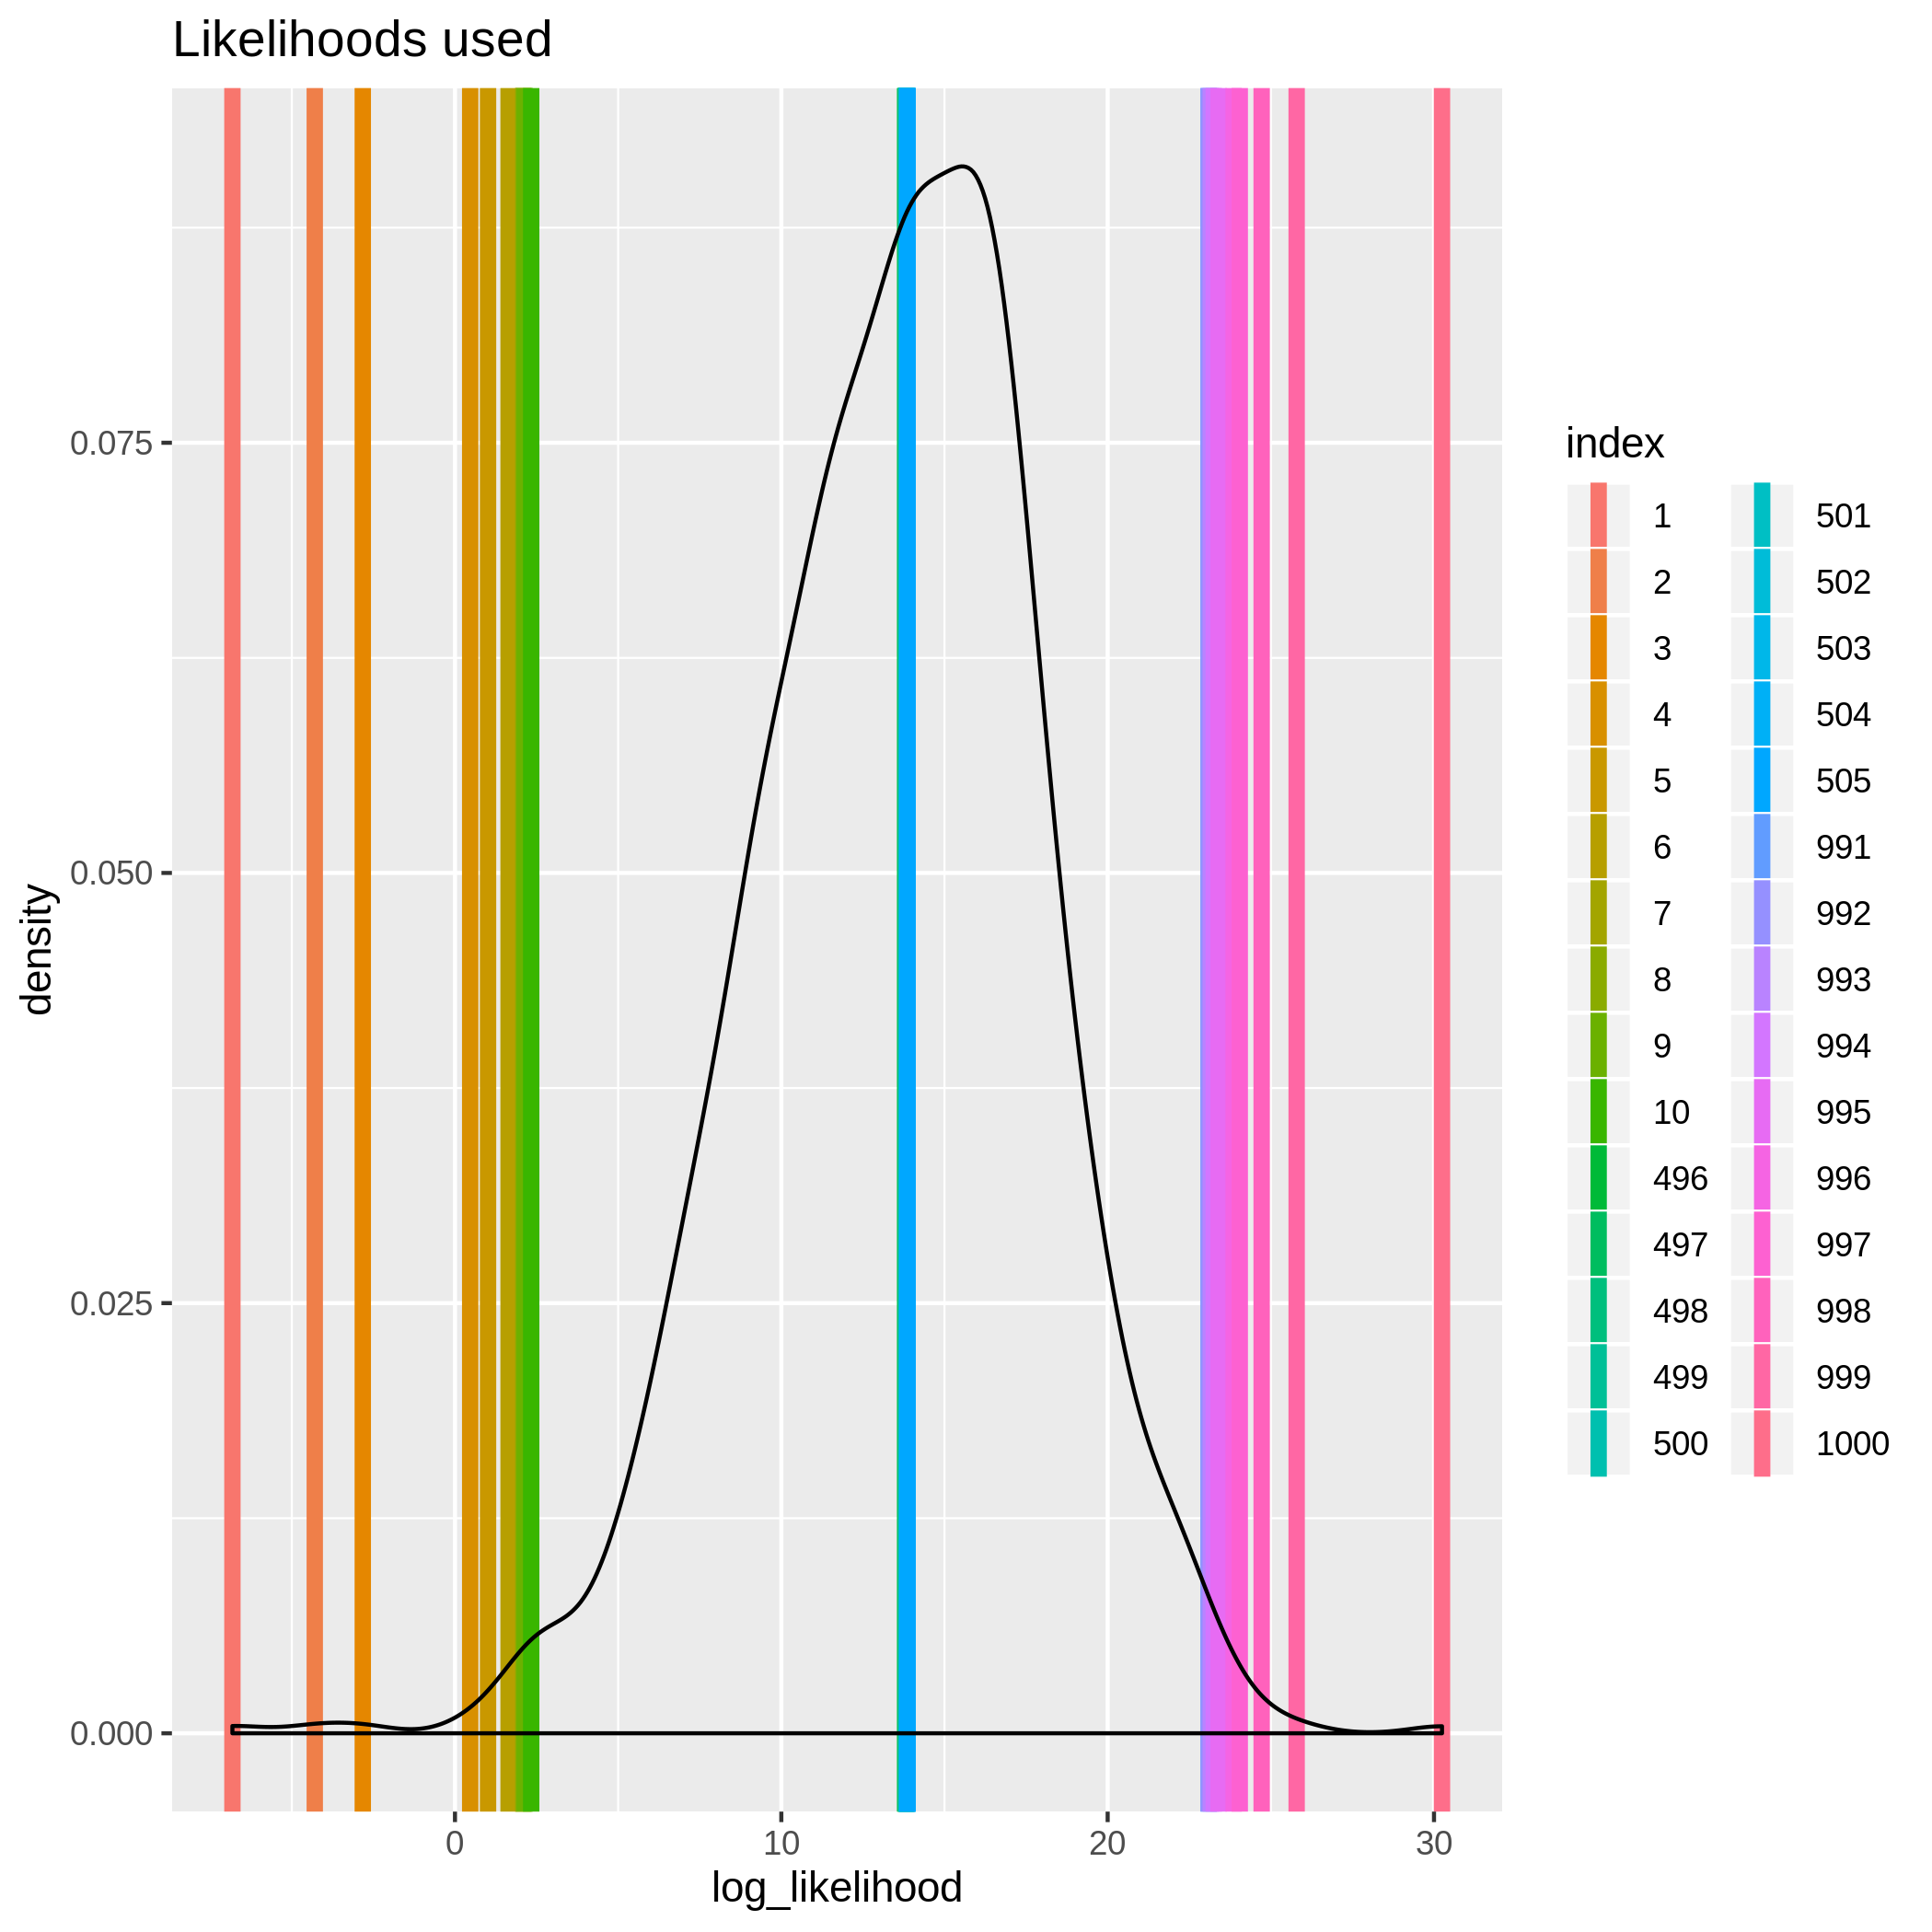
\includegraphics[width=\textwidth]{pirouette_example_23/likelihoods.png}
  \caption{Distribution of likelihoods, as well as which ones are picked}
\end{figure}

\giovanni{I like the idea of showing the likelihood shape. However I find the colored lines to be confusing. Maybe there is a clearer way to show that. I also think it is necessary to specify the parameters used, as this likelihood profile depends on them.}

%%%%%%%%%%%%%%%%%%%%%%%%%%%%%%%%%%%%%%%%%%%%%%%%%%%%%%%%%%%%%%%%%%%%%%%%%%%%%%%%
\subsection{The effect of equal or equalized mutation rate in the twin alignment}
\label{subsec:different_n_mutations}
%%%%%%%%%%%%%%%%%%%%%%%%%%%%%%%%%%%%%%%%%%%%%%%%%%%%%%%%%%%%%%%%%%%%%%%%%%%%%%%%
  
The main example uses a twin alignment that has the same number
of mutations (as measured from the ancestral sequence) as the true alignment.

Here, we show the same results, with the difference that
the twin alignment uses the same mutation rate, yet is not guaranteed
to have the same number of mutations.

The code used in this part of the article can be found at 
\url{https://github.com/richelbilderbeek/pirouette_example_18} and
\url{https://github.com/richelbilderbeek/pirouette_example_28}.

\begin{figure}[H]
  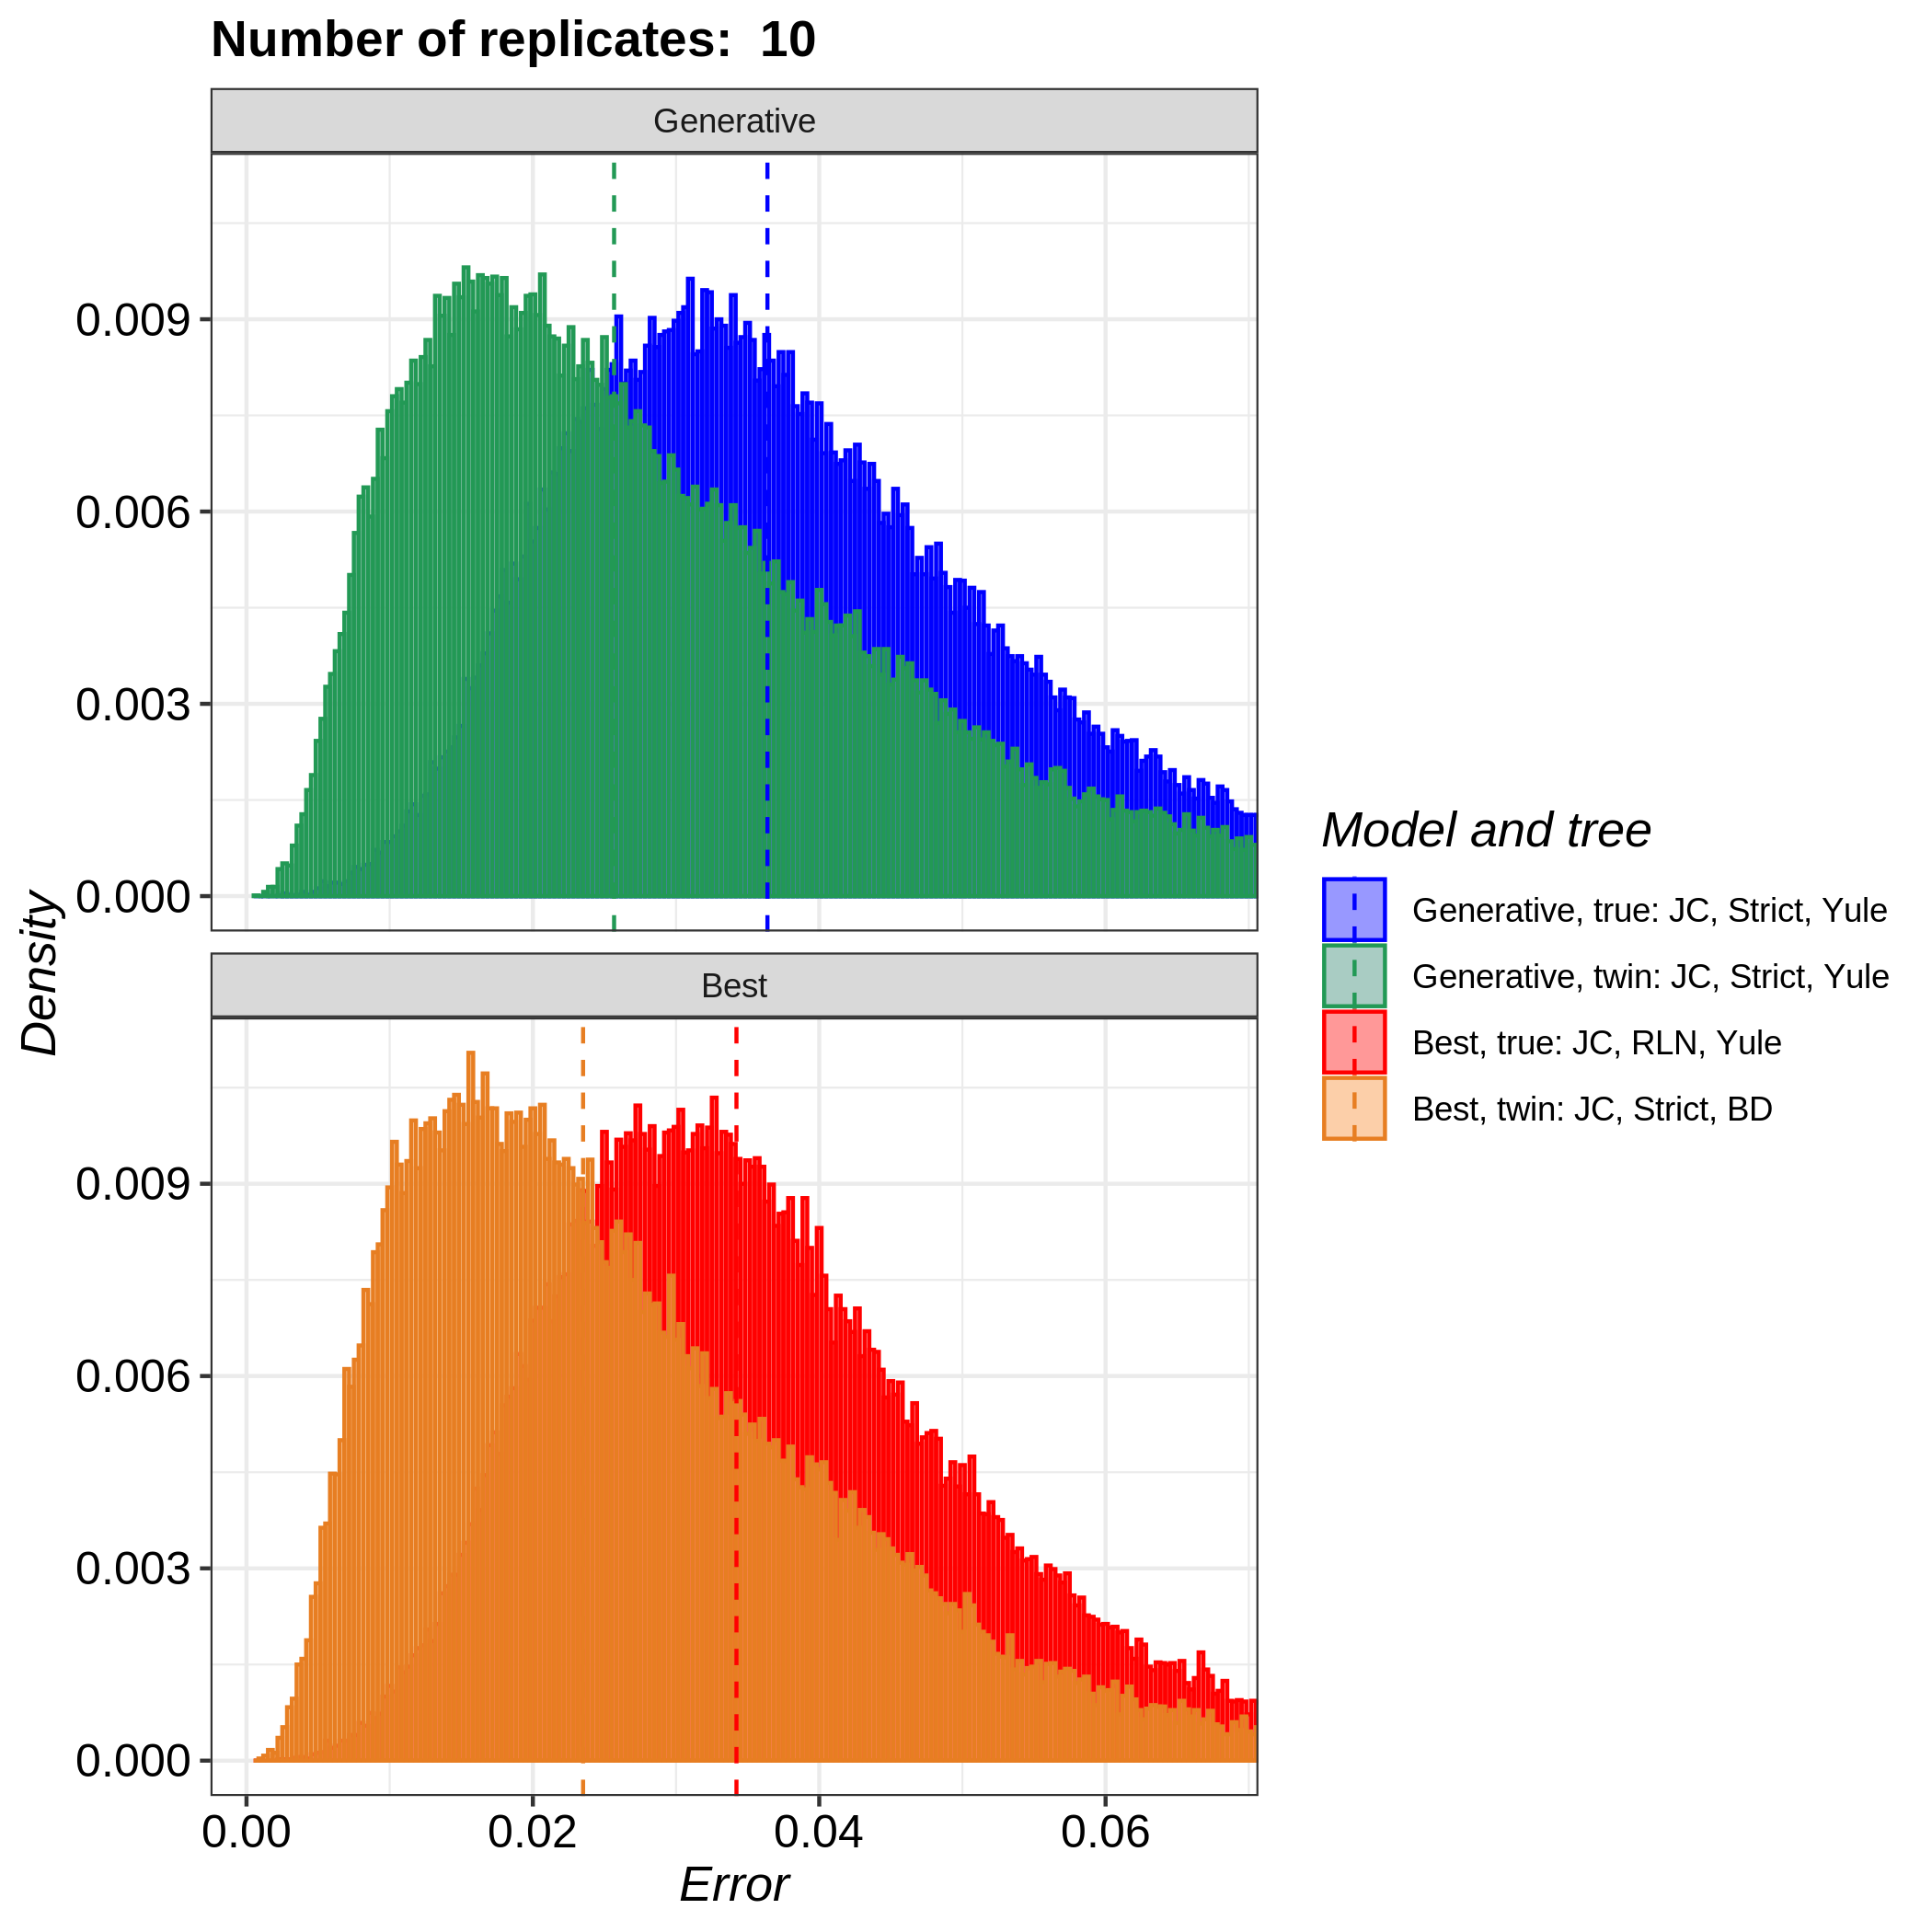
\includegraphics[width=\textwidth]{pirouette_example_18/errors.png}
  \caption{Equal mutation rate, 10 hours}
\end{figure}

\begin{figure}[H]
  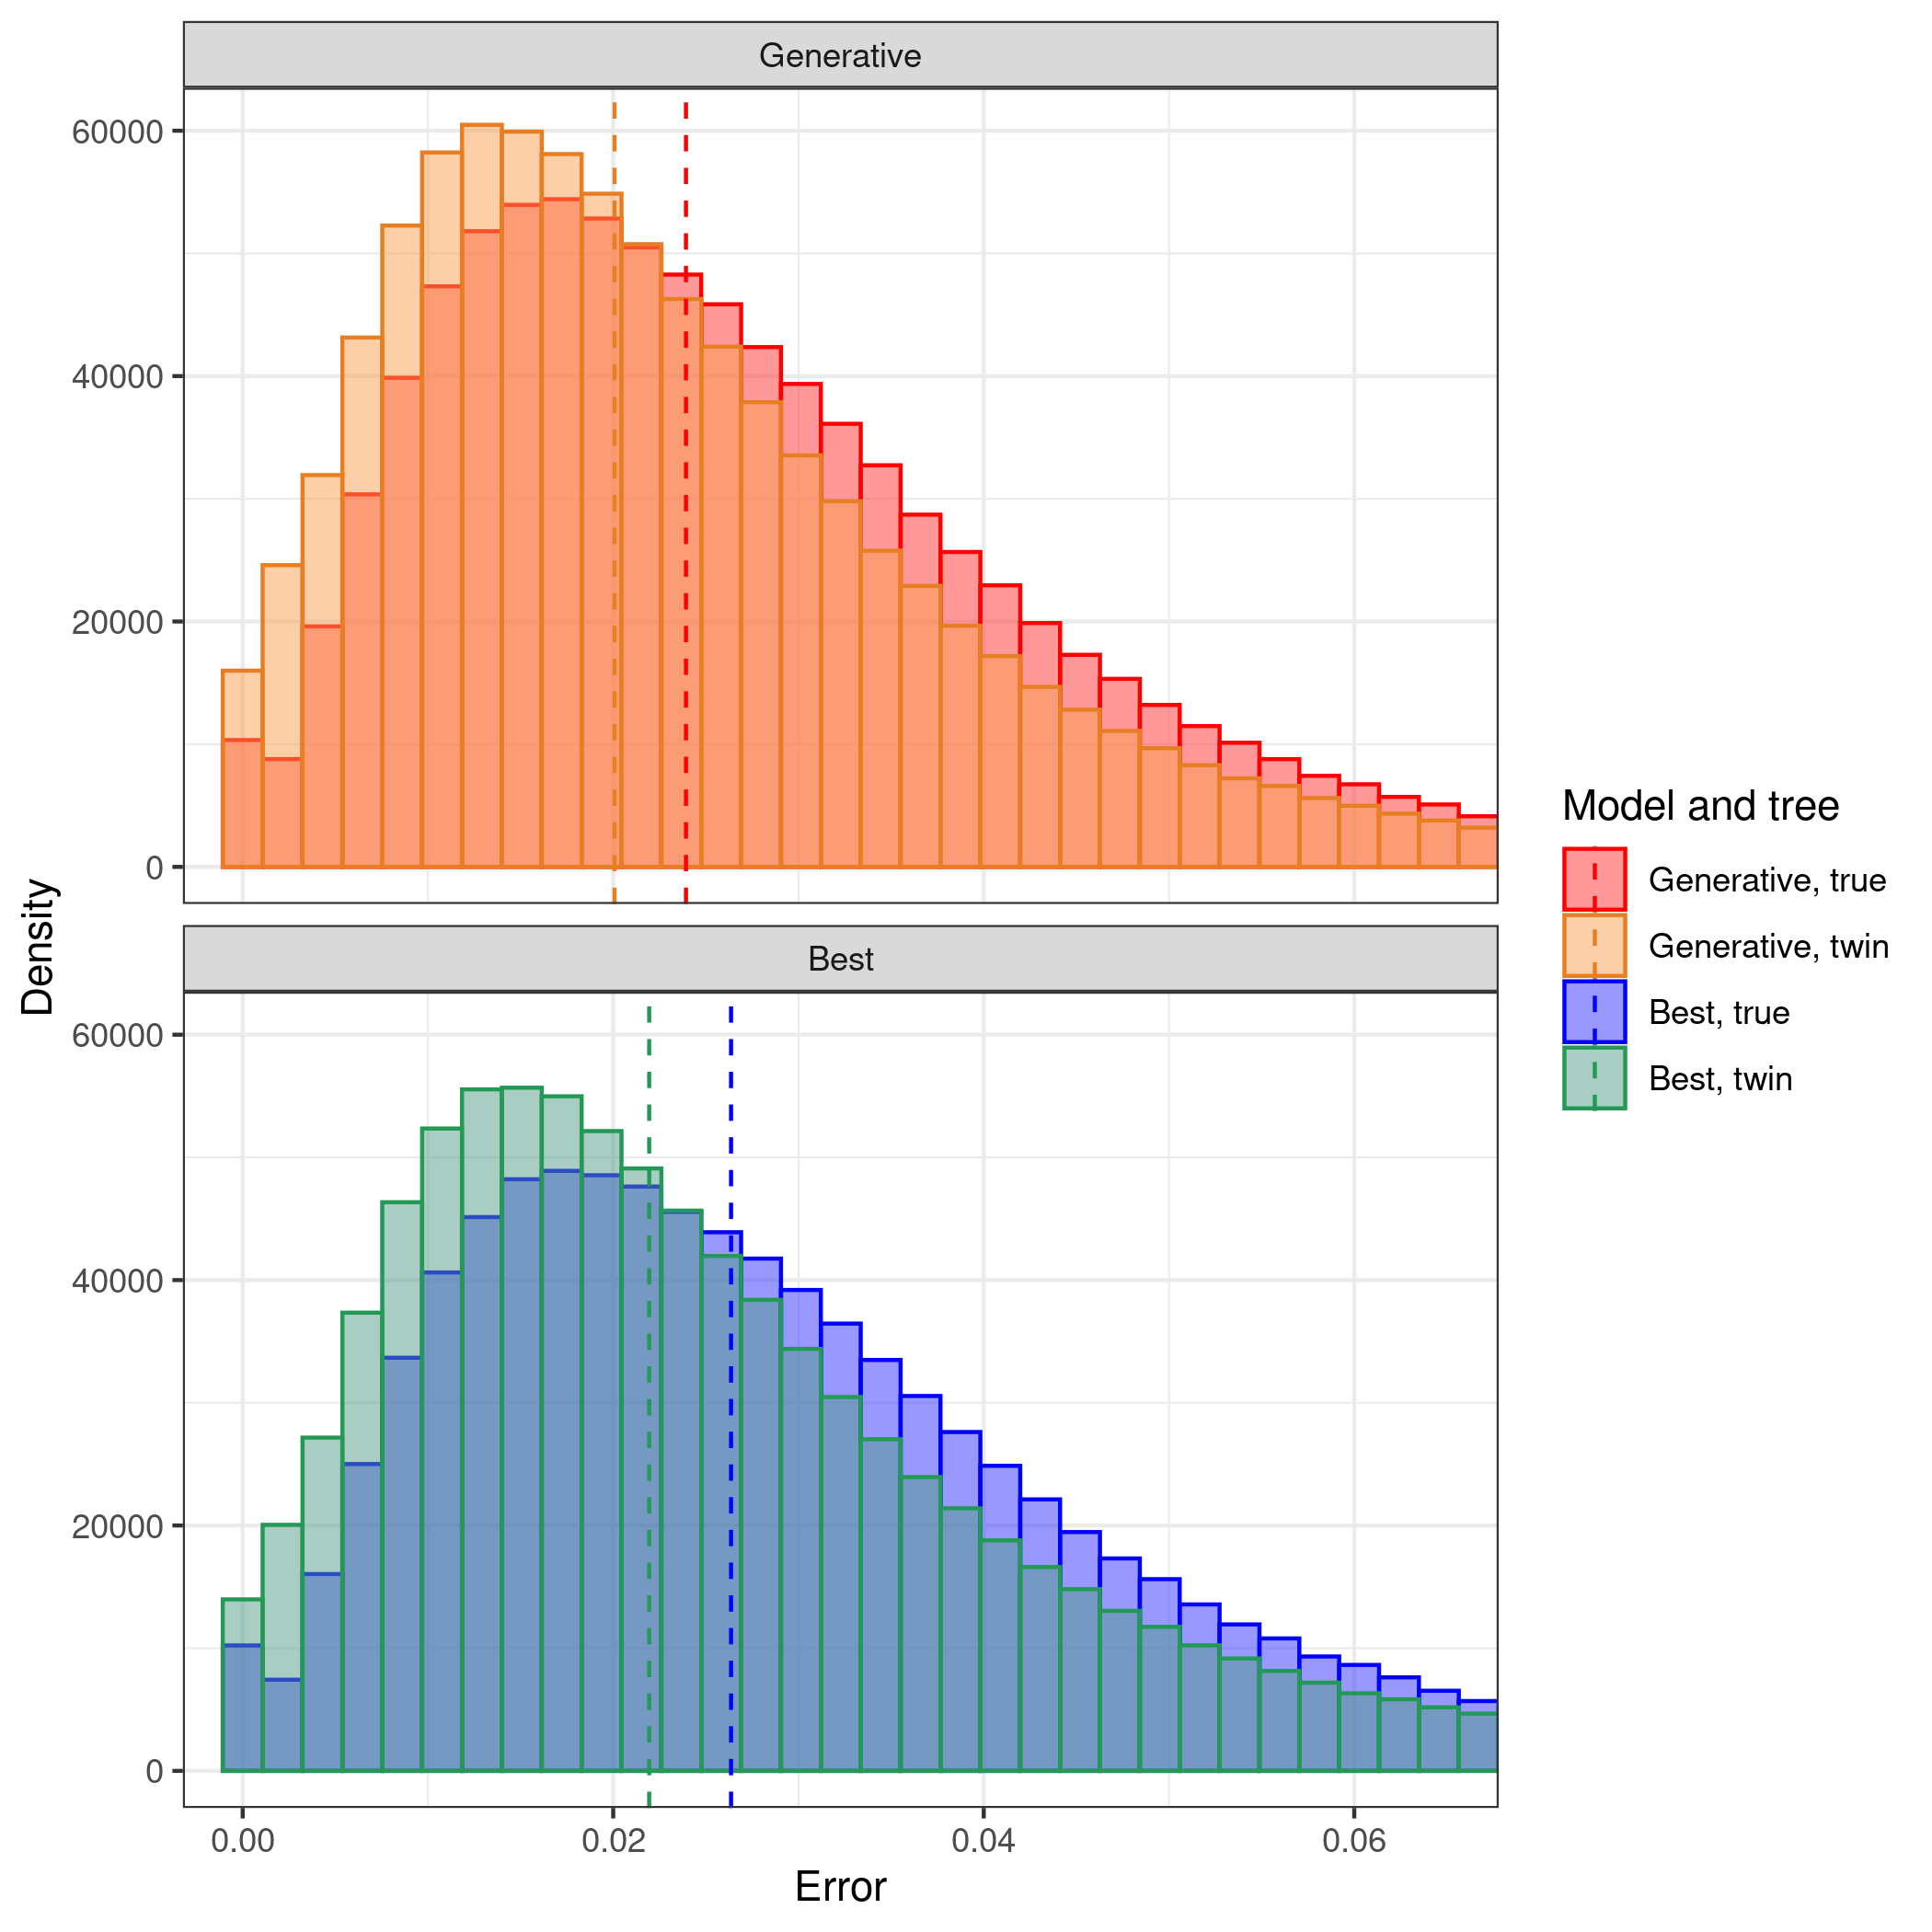
\includegraphics[width=\textwidth]{pirouette_example_28/errors.png}
  \caption{Equal mutation rate and number of mutations, 16 hours (main example)}
\end{figure}

%%%%%%%%%%%%%%%%%%%%%%%%%%%%%%%%%%%%%%%%%%%%%%%%%%%%%%%%%%%%%%%%%%%%%%%%%%%%%%%%
\subsection{The effect of mutation rate}
\label{subsec:mutation_rate}
%%%%%%%%%%%%%%%%%%%%%%%%%%%%%%%%%%%%%%%%%%%%%%%%%%%%%%%%%%%%%%%%%%%%%%%%%%%%%%%%

The main example uses a mutation rate such that all nucleotides,
on average, mutate once over the history going from the
ancestral sequence at the crown to the alignments at the tips.
In this way, the alignment is expected to contain the maximum
amount of information.

Here, we show the same results, with the only difference that
the mutations rates are changed.
For a lower mutation rate, less mutations will be observed, thus
genetic information will be less, thus the inference is expected
to go worse, thus the errors are expected to increase.
For a lower mutation rate, more double-mutations will occur,
scrambling the alignments, resulting in less genetic information, 
thus the inference is expected to go worse, 
thus the errors are expected to increase.

The code used in this part of the article can be found at 
\url{https://github.com/richelbilderbeek/pirouette_example_35} (0.25 / crown age),
\url{https://github.com/richelbilderbeek/pirouette_example_36} (0.50 / crown age),
\url{https://github.com/richelbilderbeek/pirouette_example_37} (0.75 / crown age),
\url{https://github.com/richelbilderbeek/pirouette_example_28} (1.00 / crown age, main example),
\url{https://github.com/richelbilderbeek/pirouette_example_38} (1.25 / crown age),
\url{https://github.com/richelbilderbeek/pirouette_example_39} (1.50 / crown age),
\url{https://github.com/richelbilderbeek/pirouette_example_40} (2.00 / crown age),

\begin{figure}[H]
  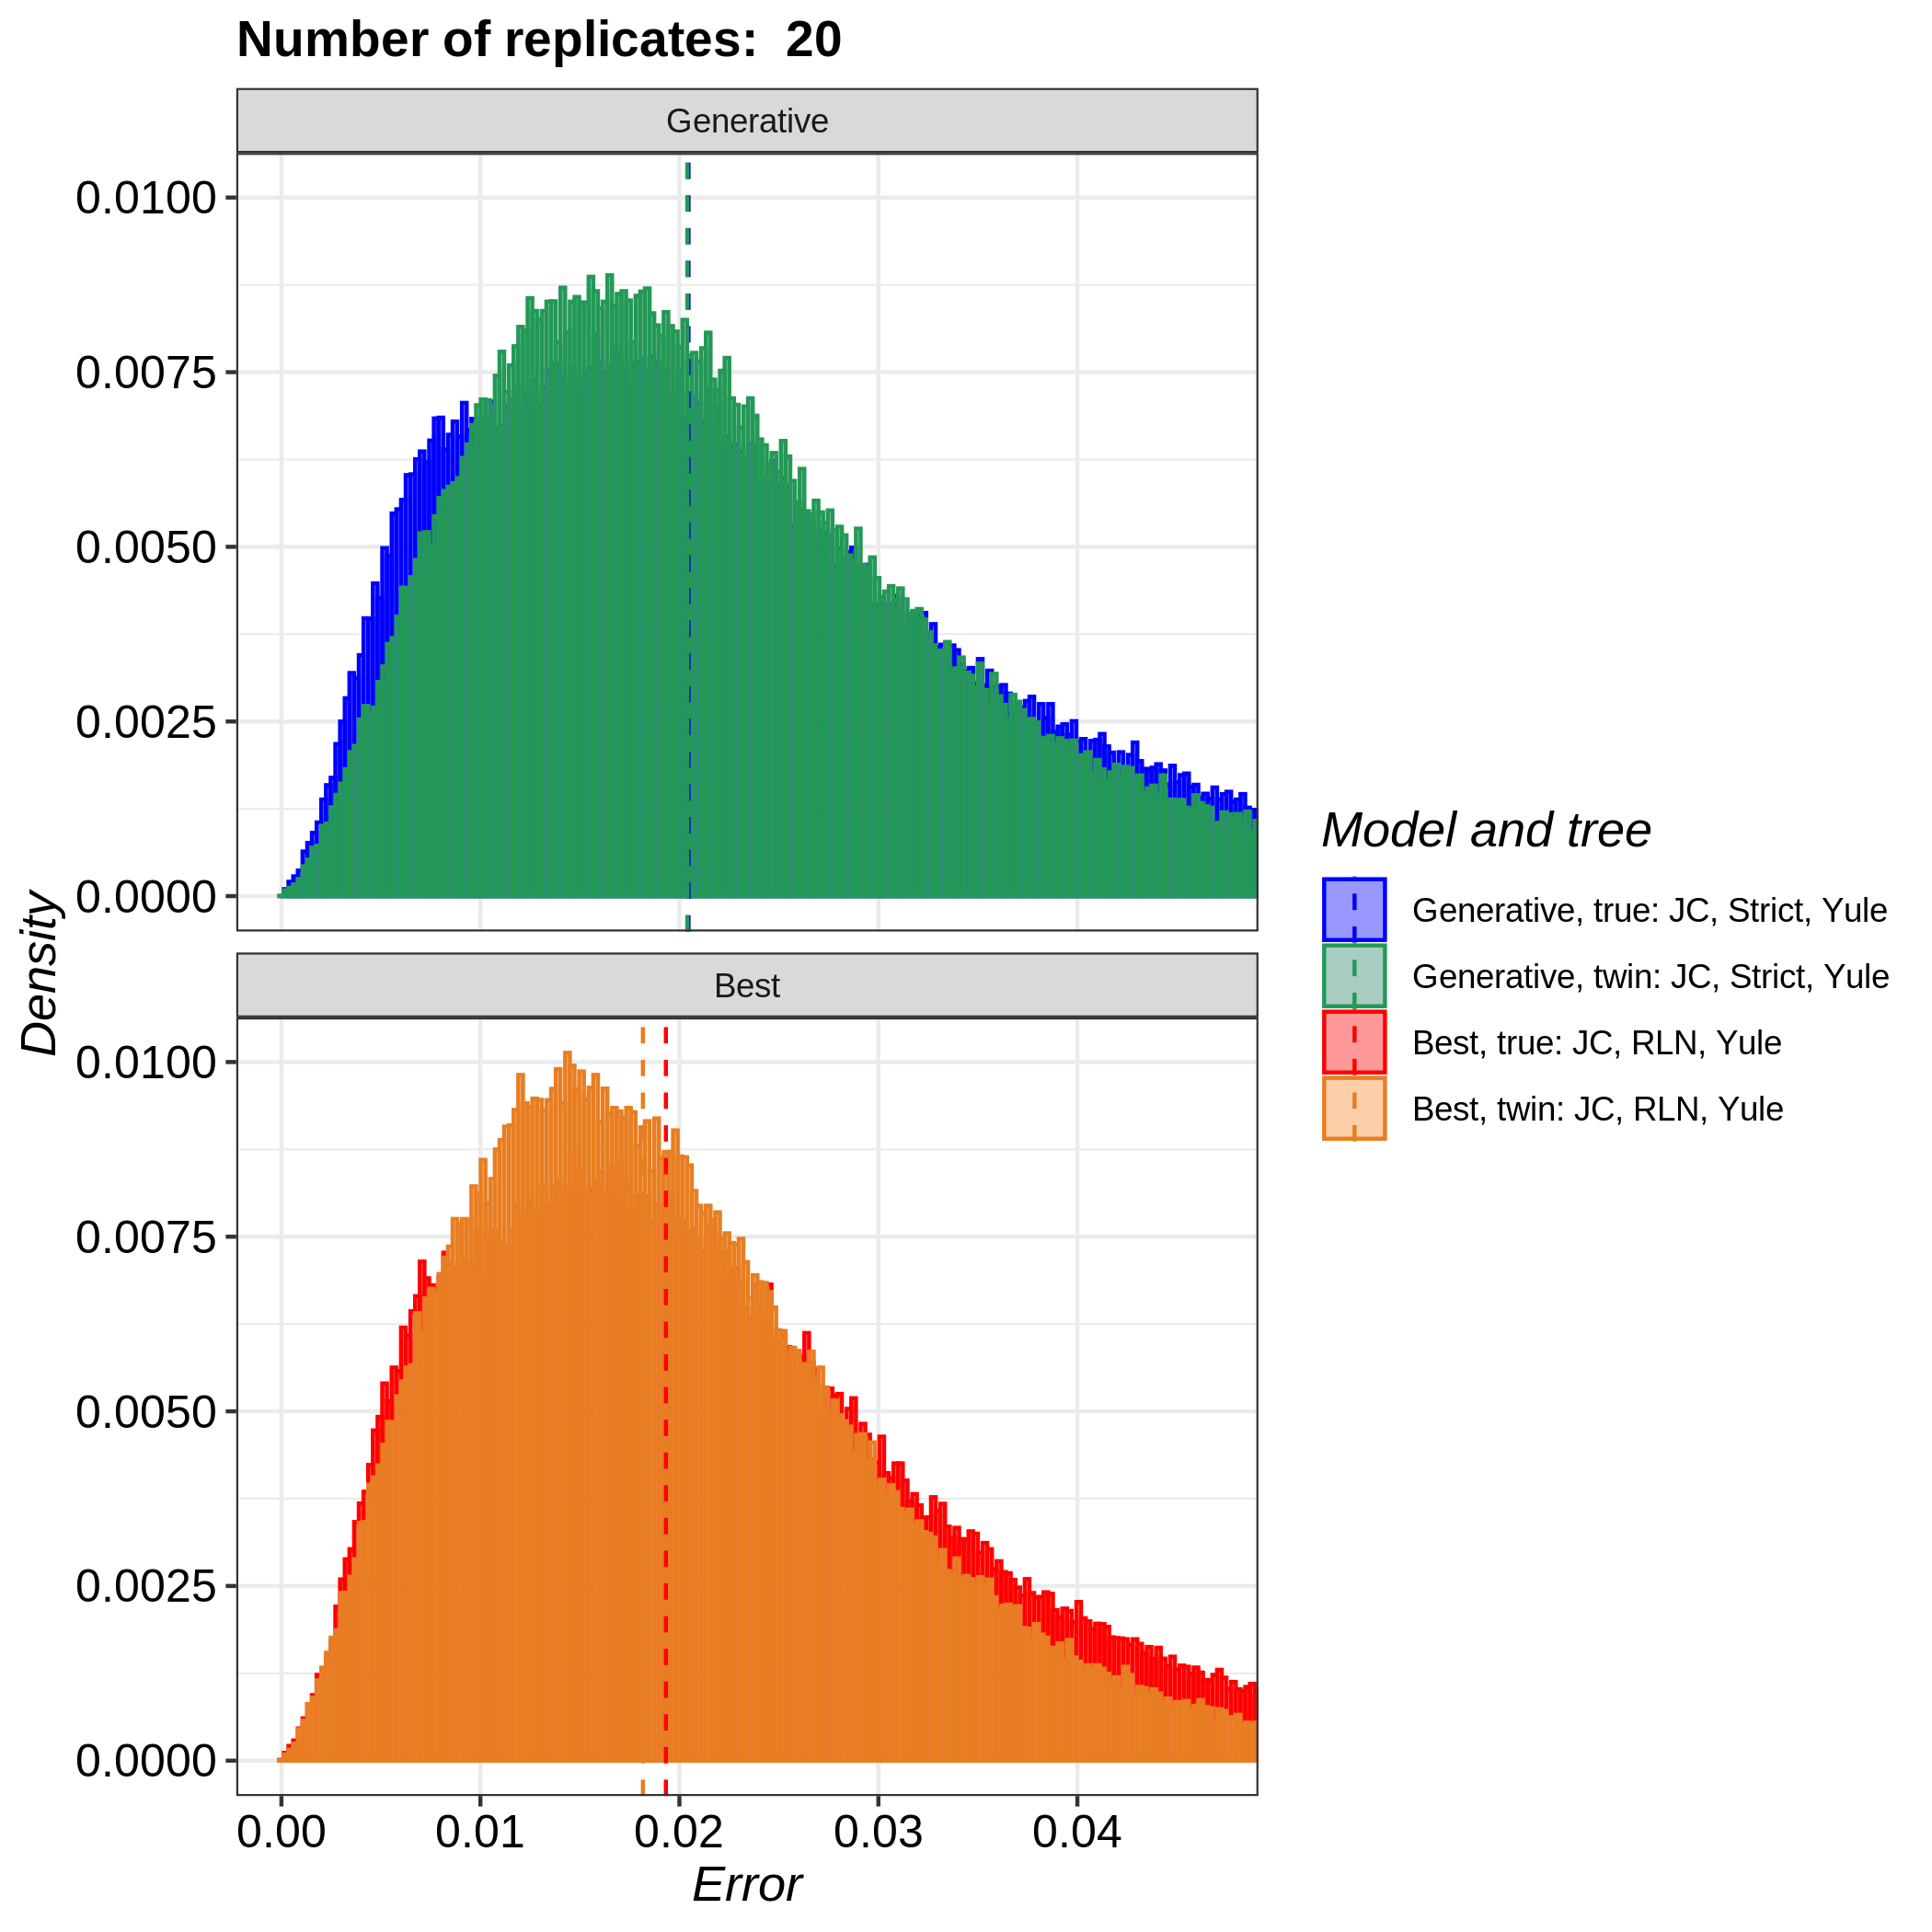
\includegraphics[width=\textwidth]{pirouette_example_35/errors.png}
  \caption{Per-nucleotide mutation rate of 0.25 / crown age, 11 hours}
\end{figure}

\begin{figure}[H]
  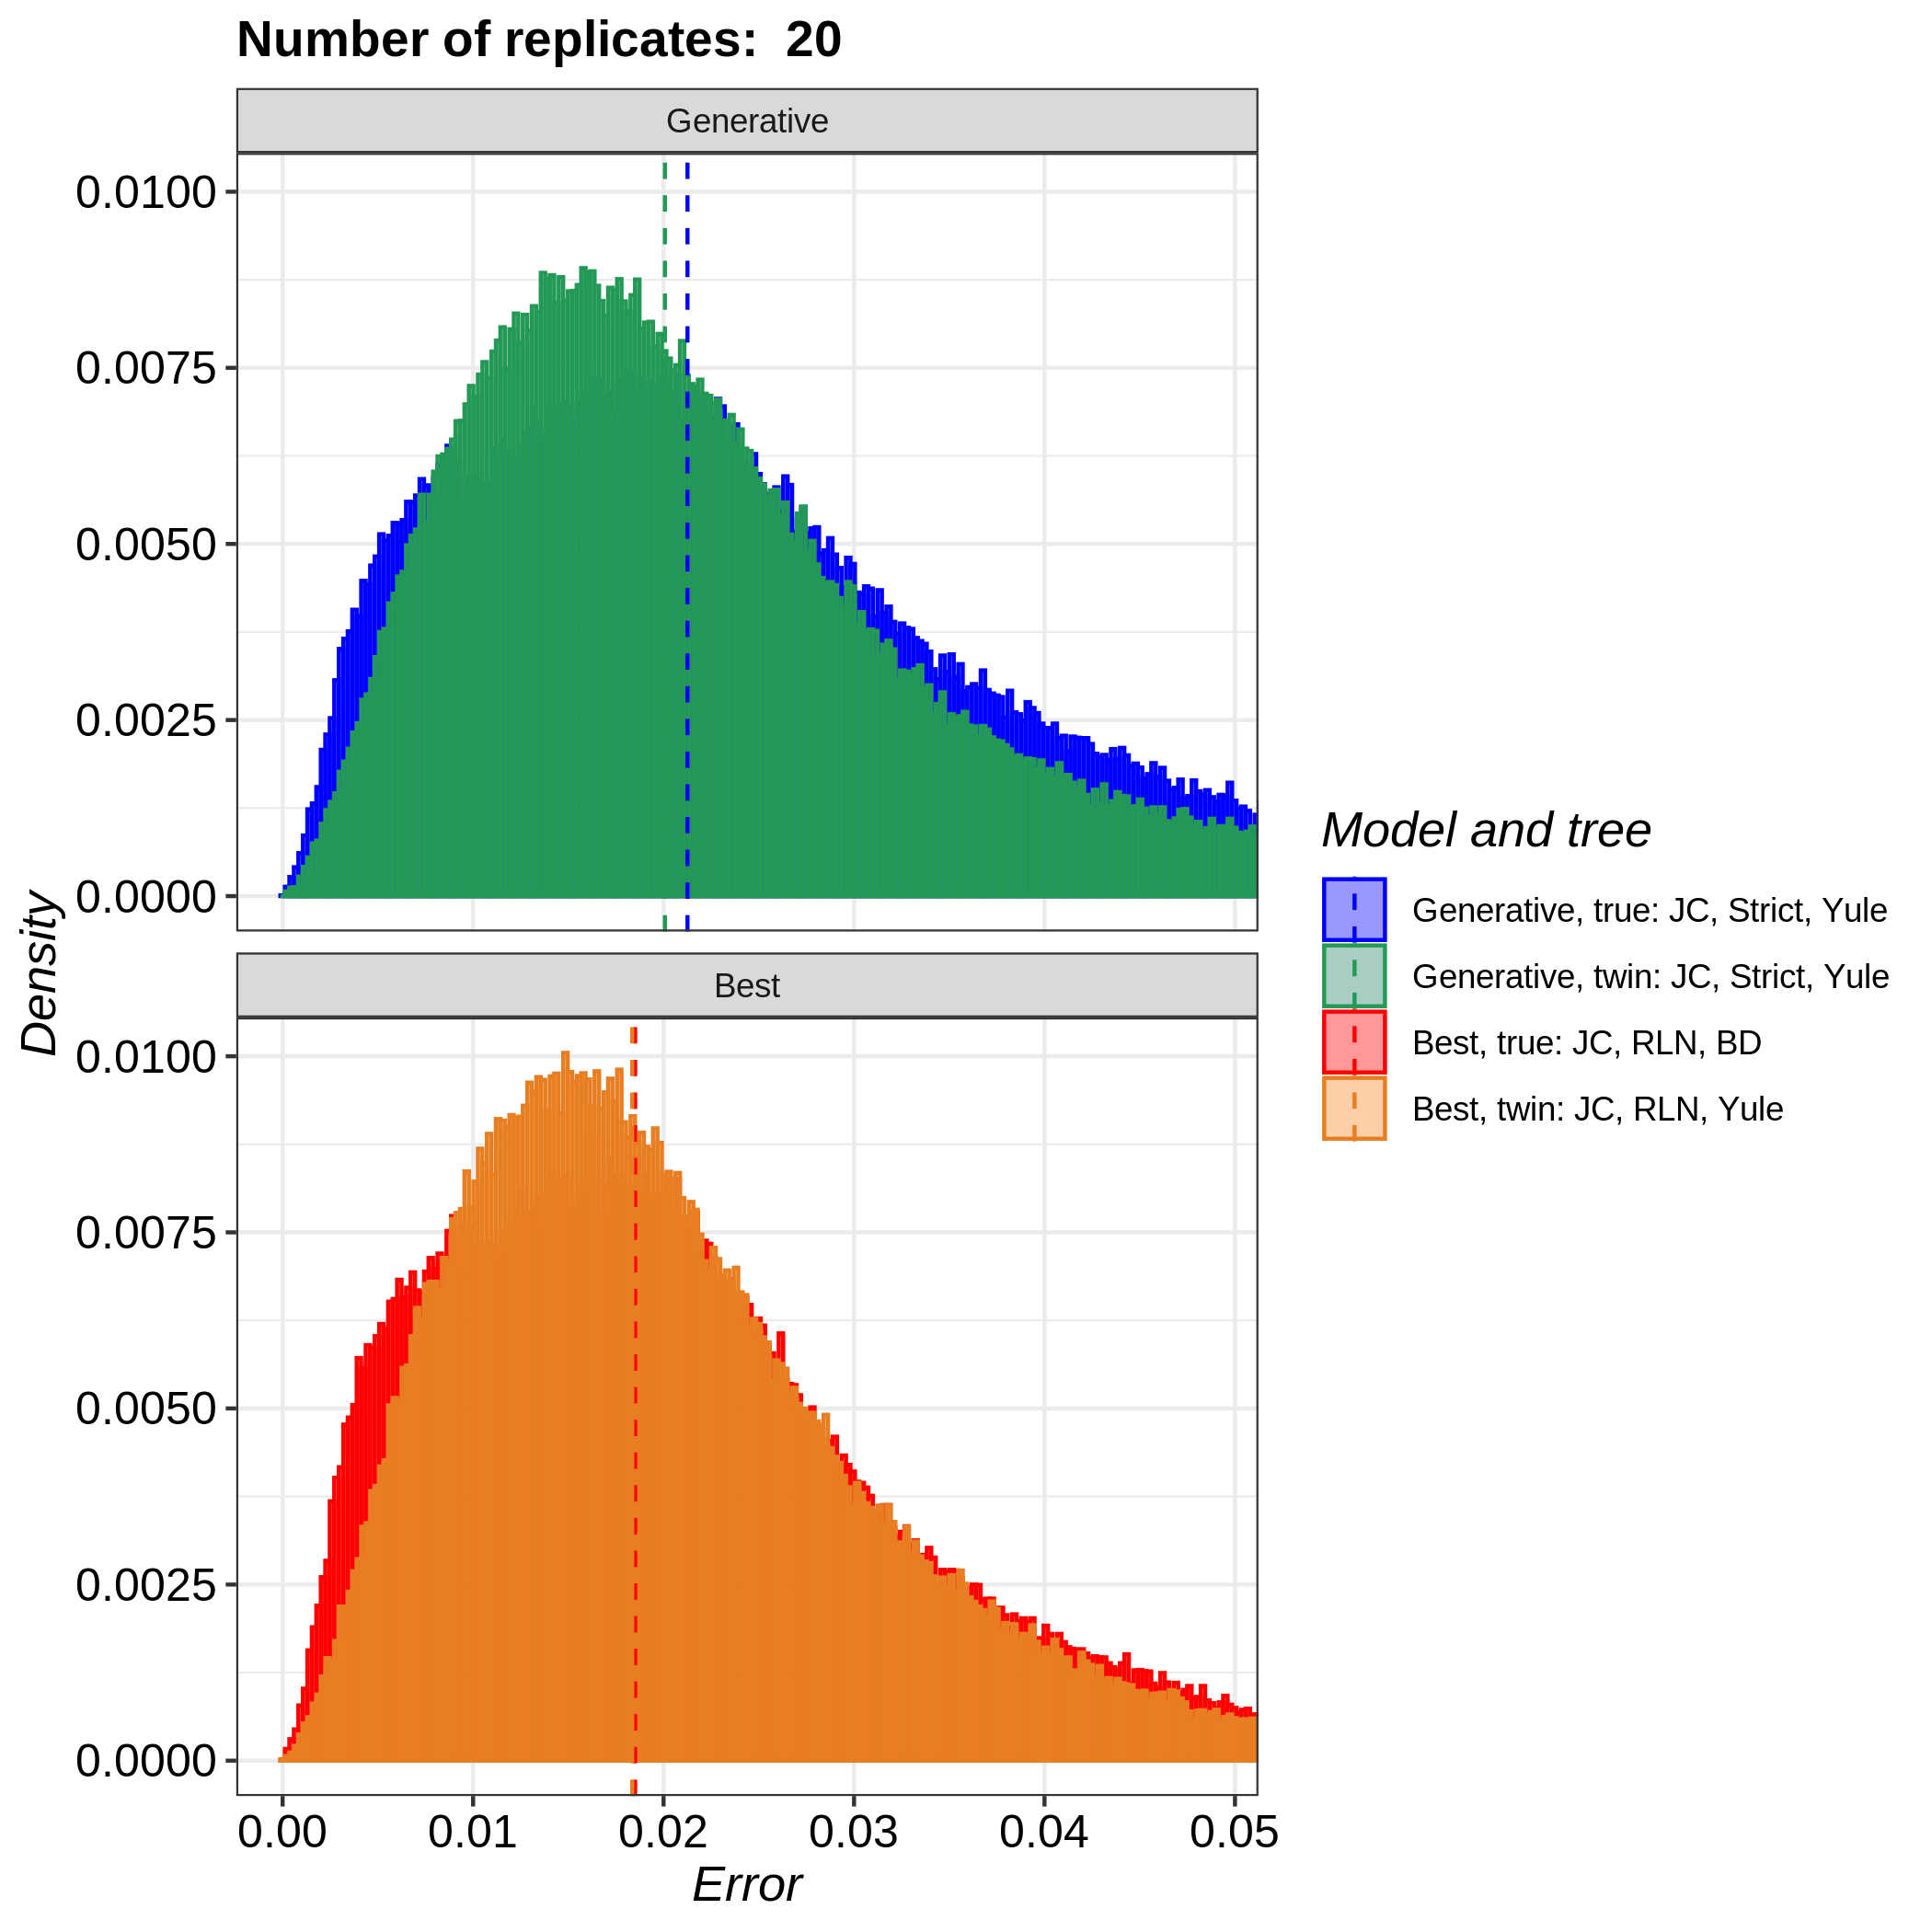
\includegraphics[width=\textwidth]{pirouette_example_36/errors.png}
  \caption{Per-nucleotide mutation rate of 0.50 / crown age, 14 hours}
\end{figure}

\begin{figure}[H]
  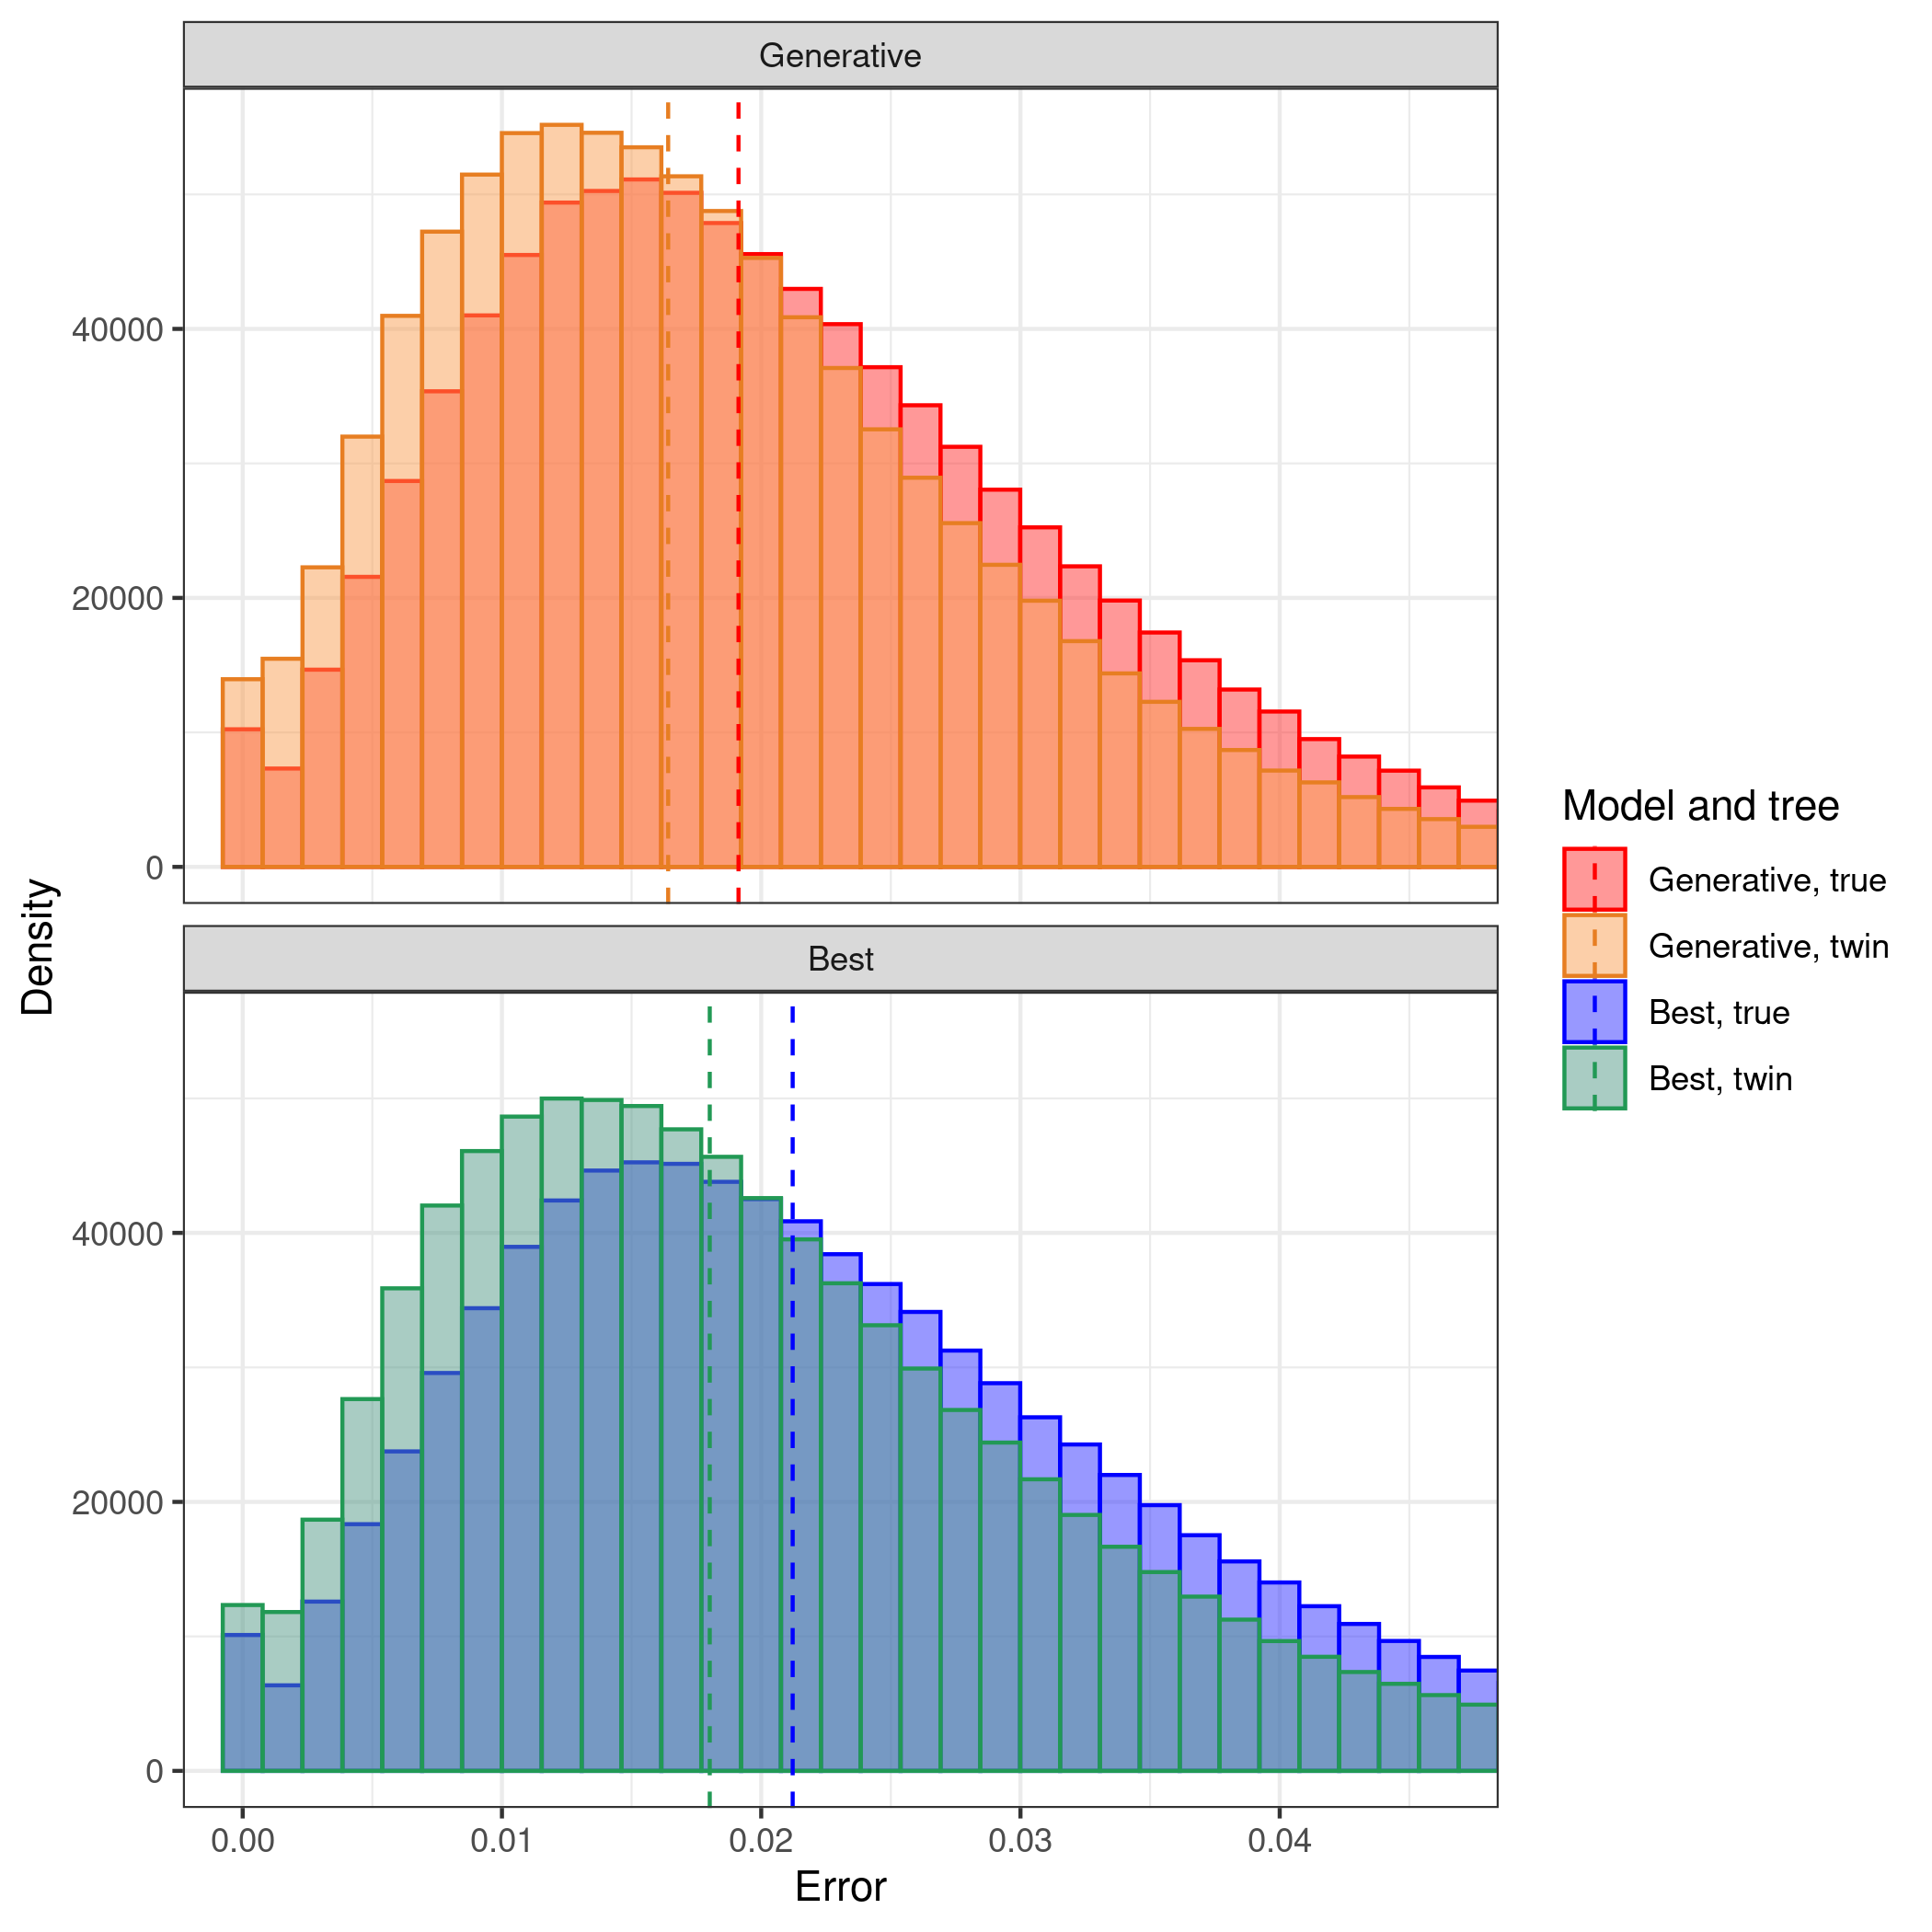
\includegraphics[width=\textwidth]{pirouette_example_37/errors.png}
  \caption{Per-nucleotide mutation rate of 0.75 / crown age, 16 hours}
\end{figure}

\begin{figure}[H]
  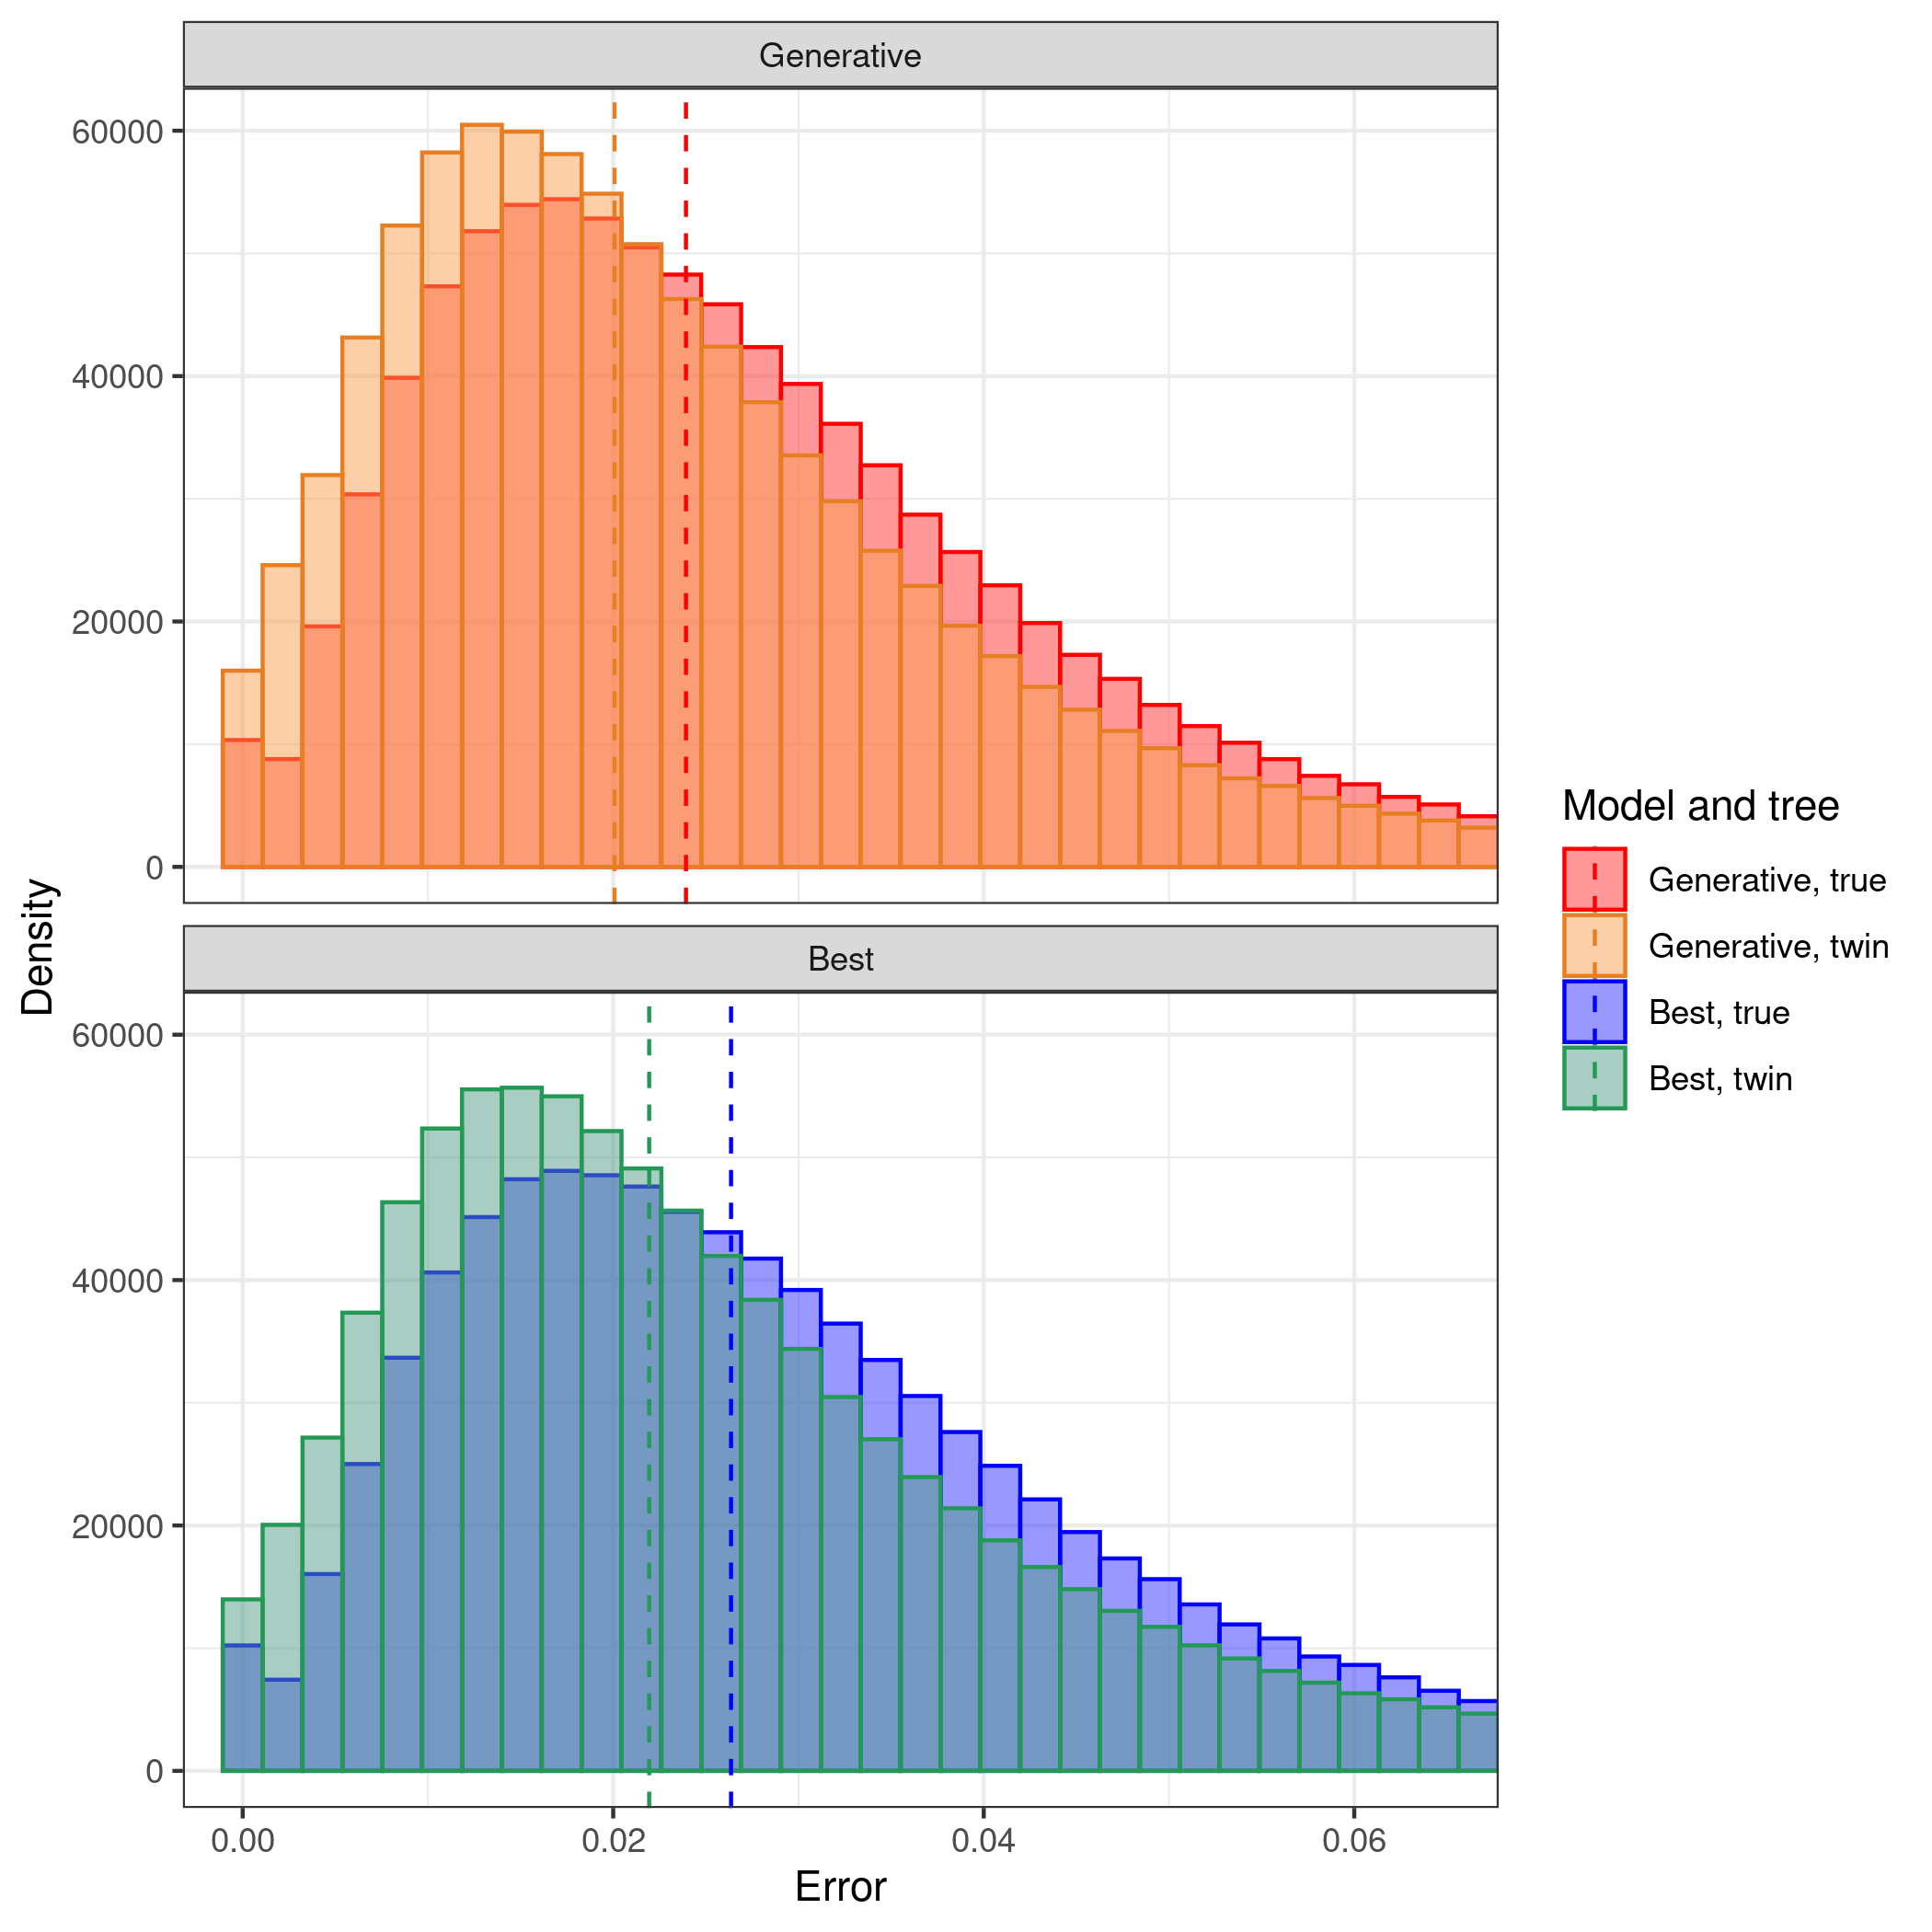
\includegraphics[width=\textwidth]{pirouette_example_28/errors.png}
  \caption{Per-nucleotide mutation rate of 1.0 / crown age, 16 hours (main example)}
\end{figure}

\begin{figure}[H]
  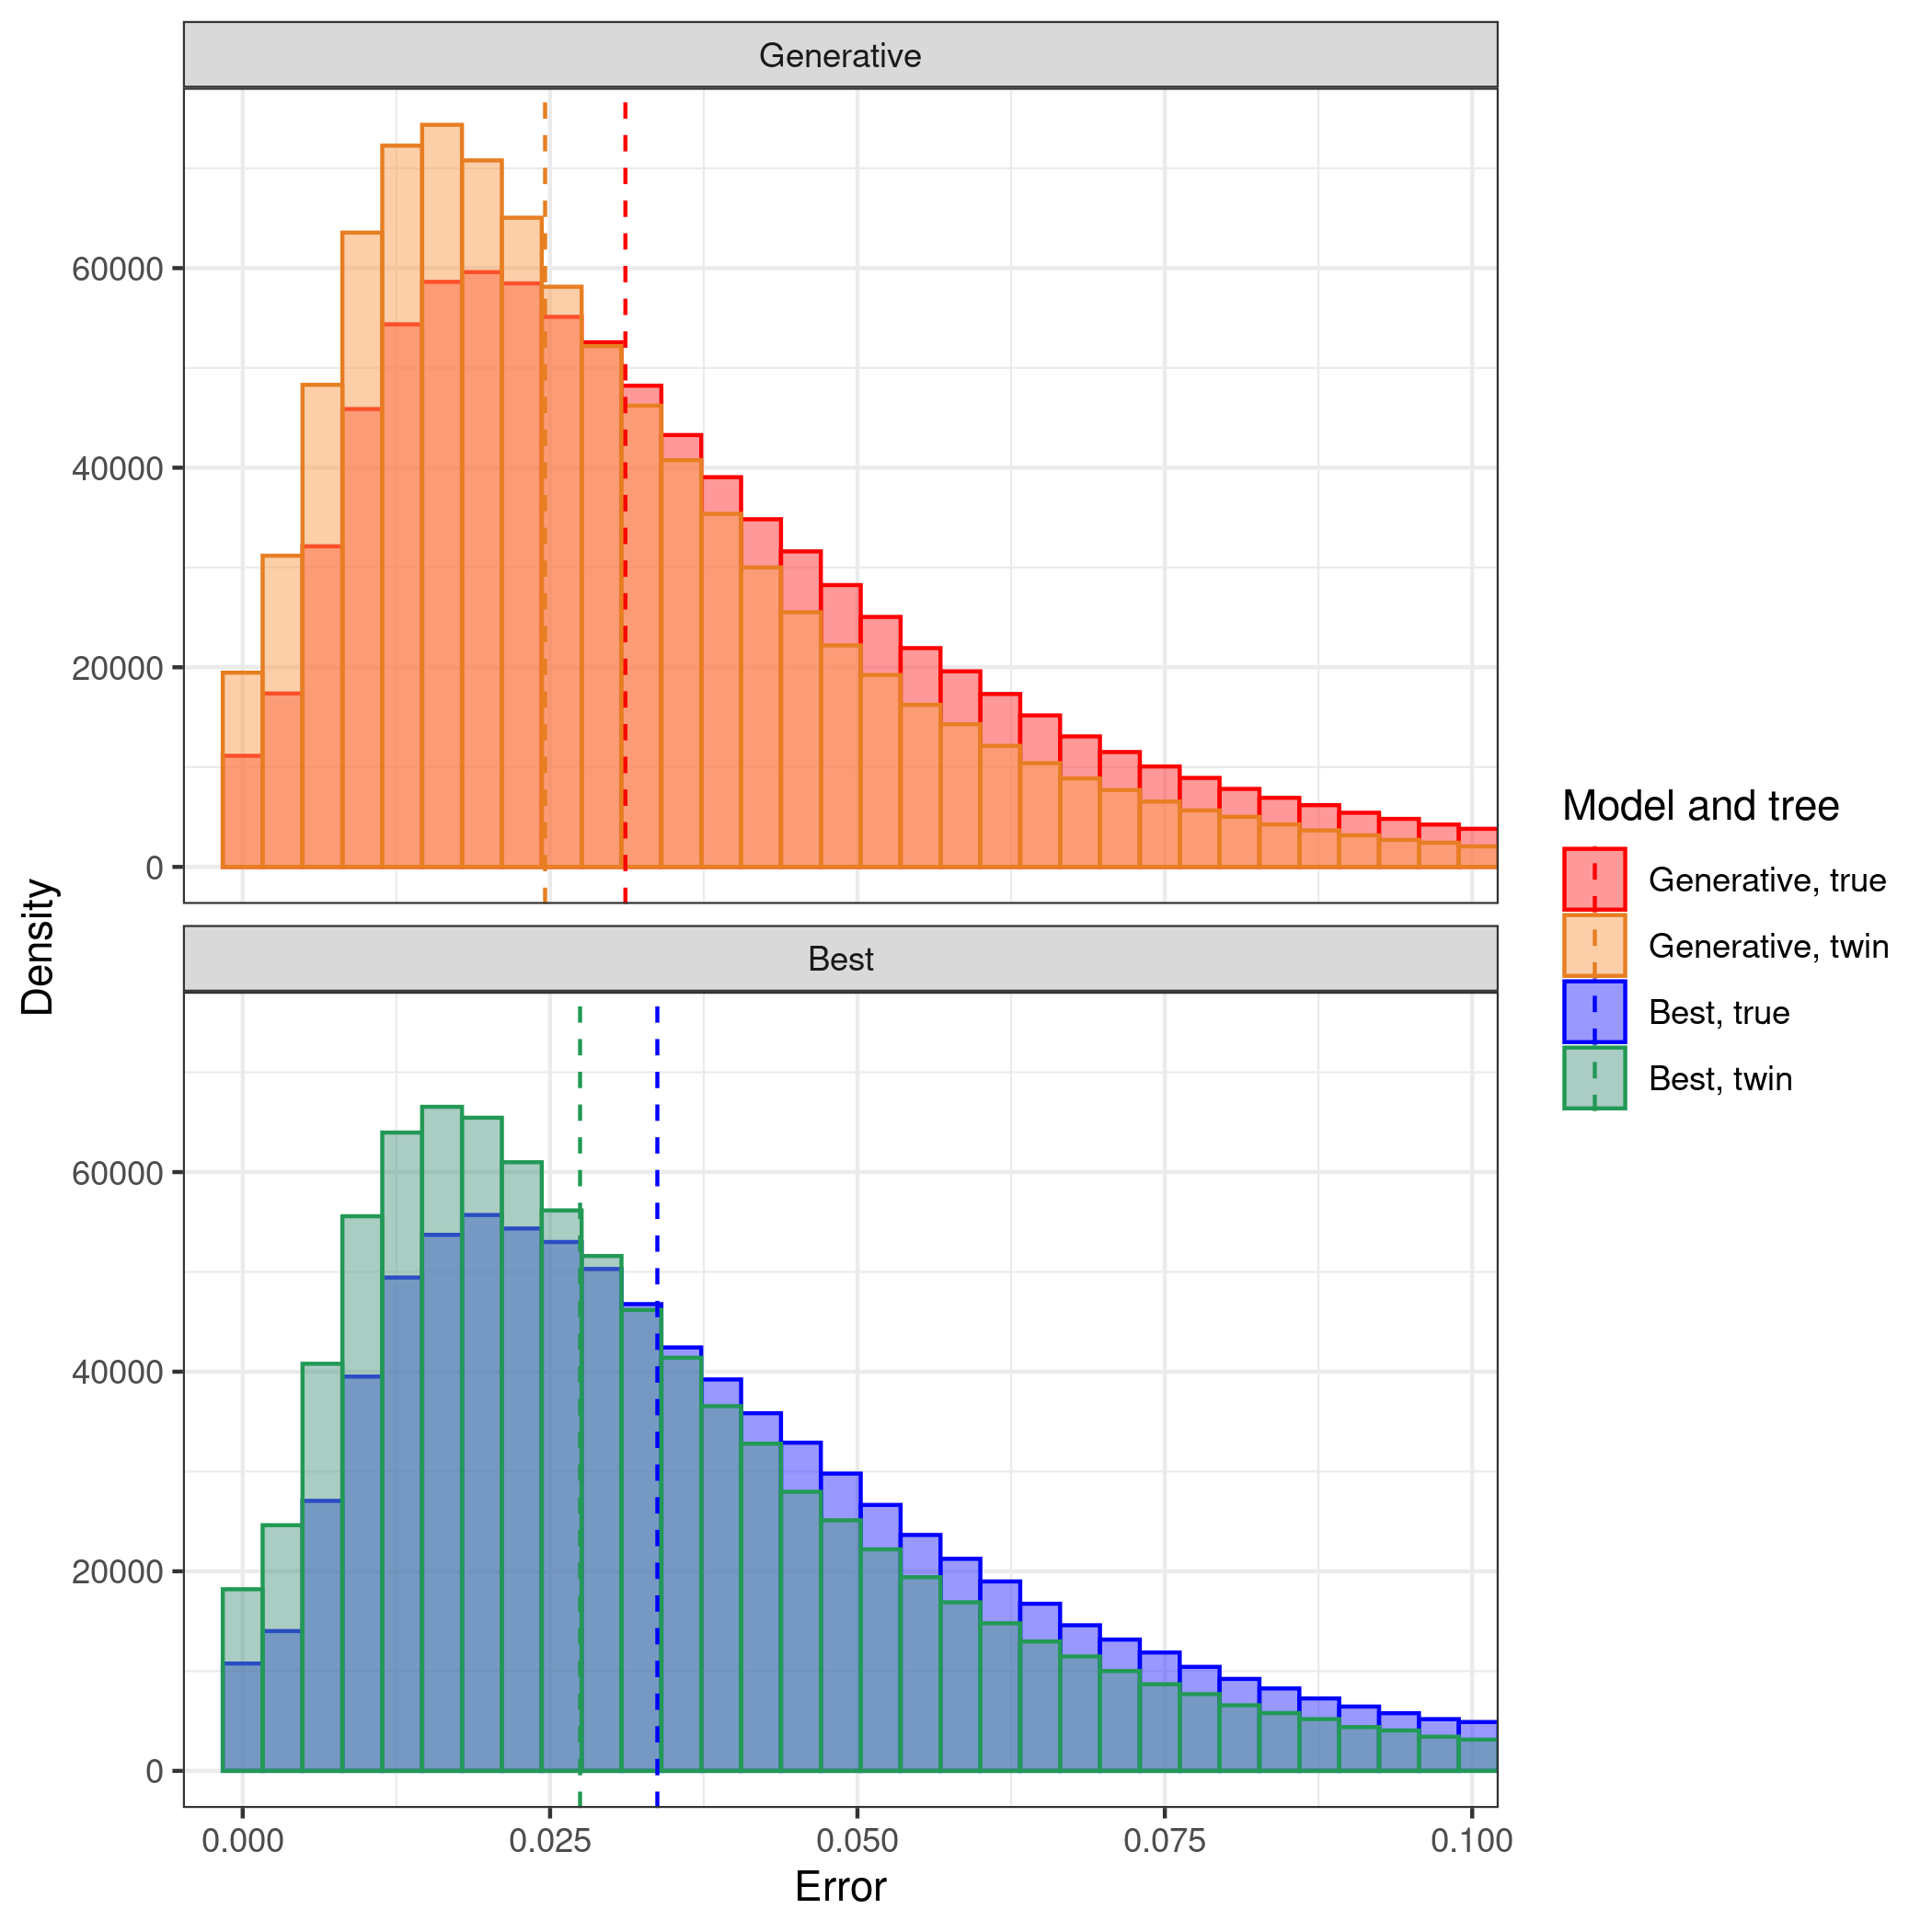
\includegraphics[width=\textwidth]{pirouette_example_38/errors.png}
  \caption{Per-nucleotide mutation rate of 1.25 / crown age, 17 hours}
\end{figure}

\begin{figure}[H]
  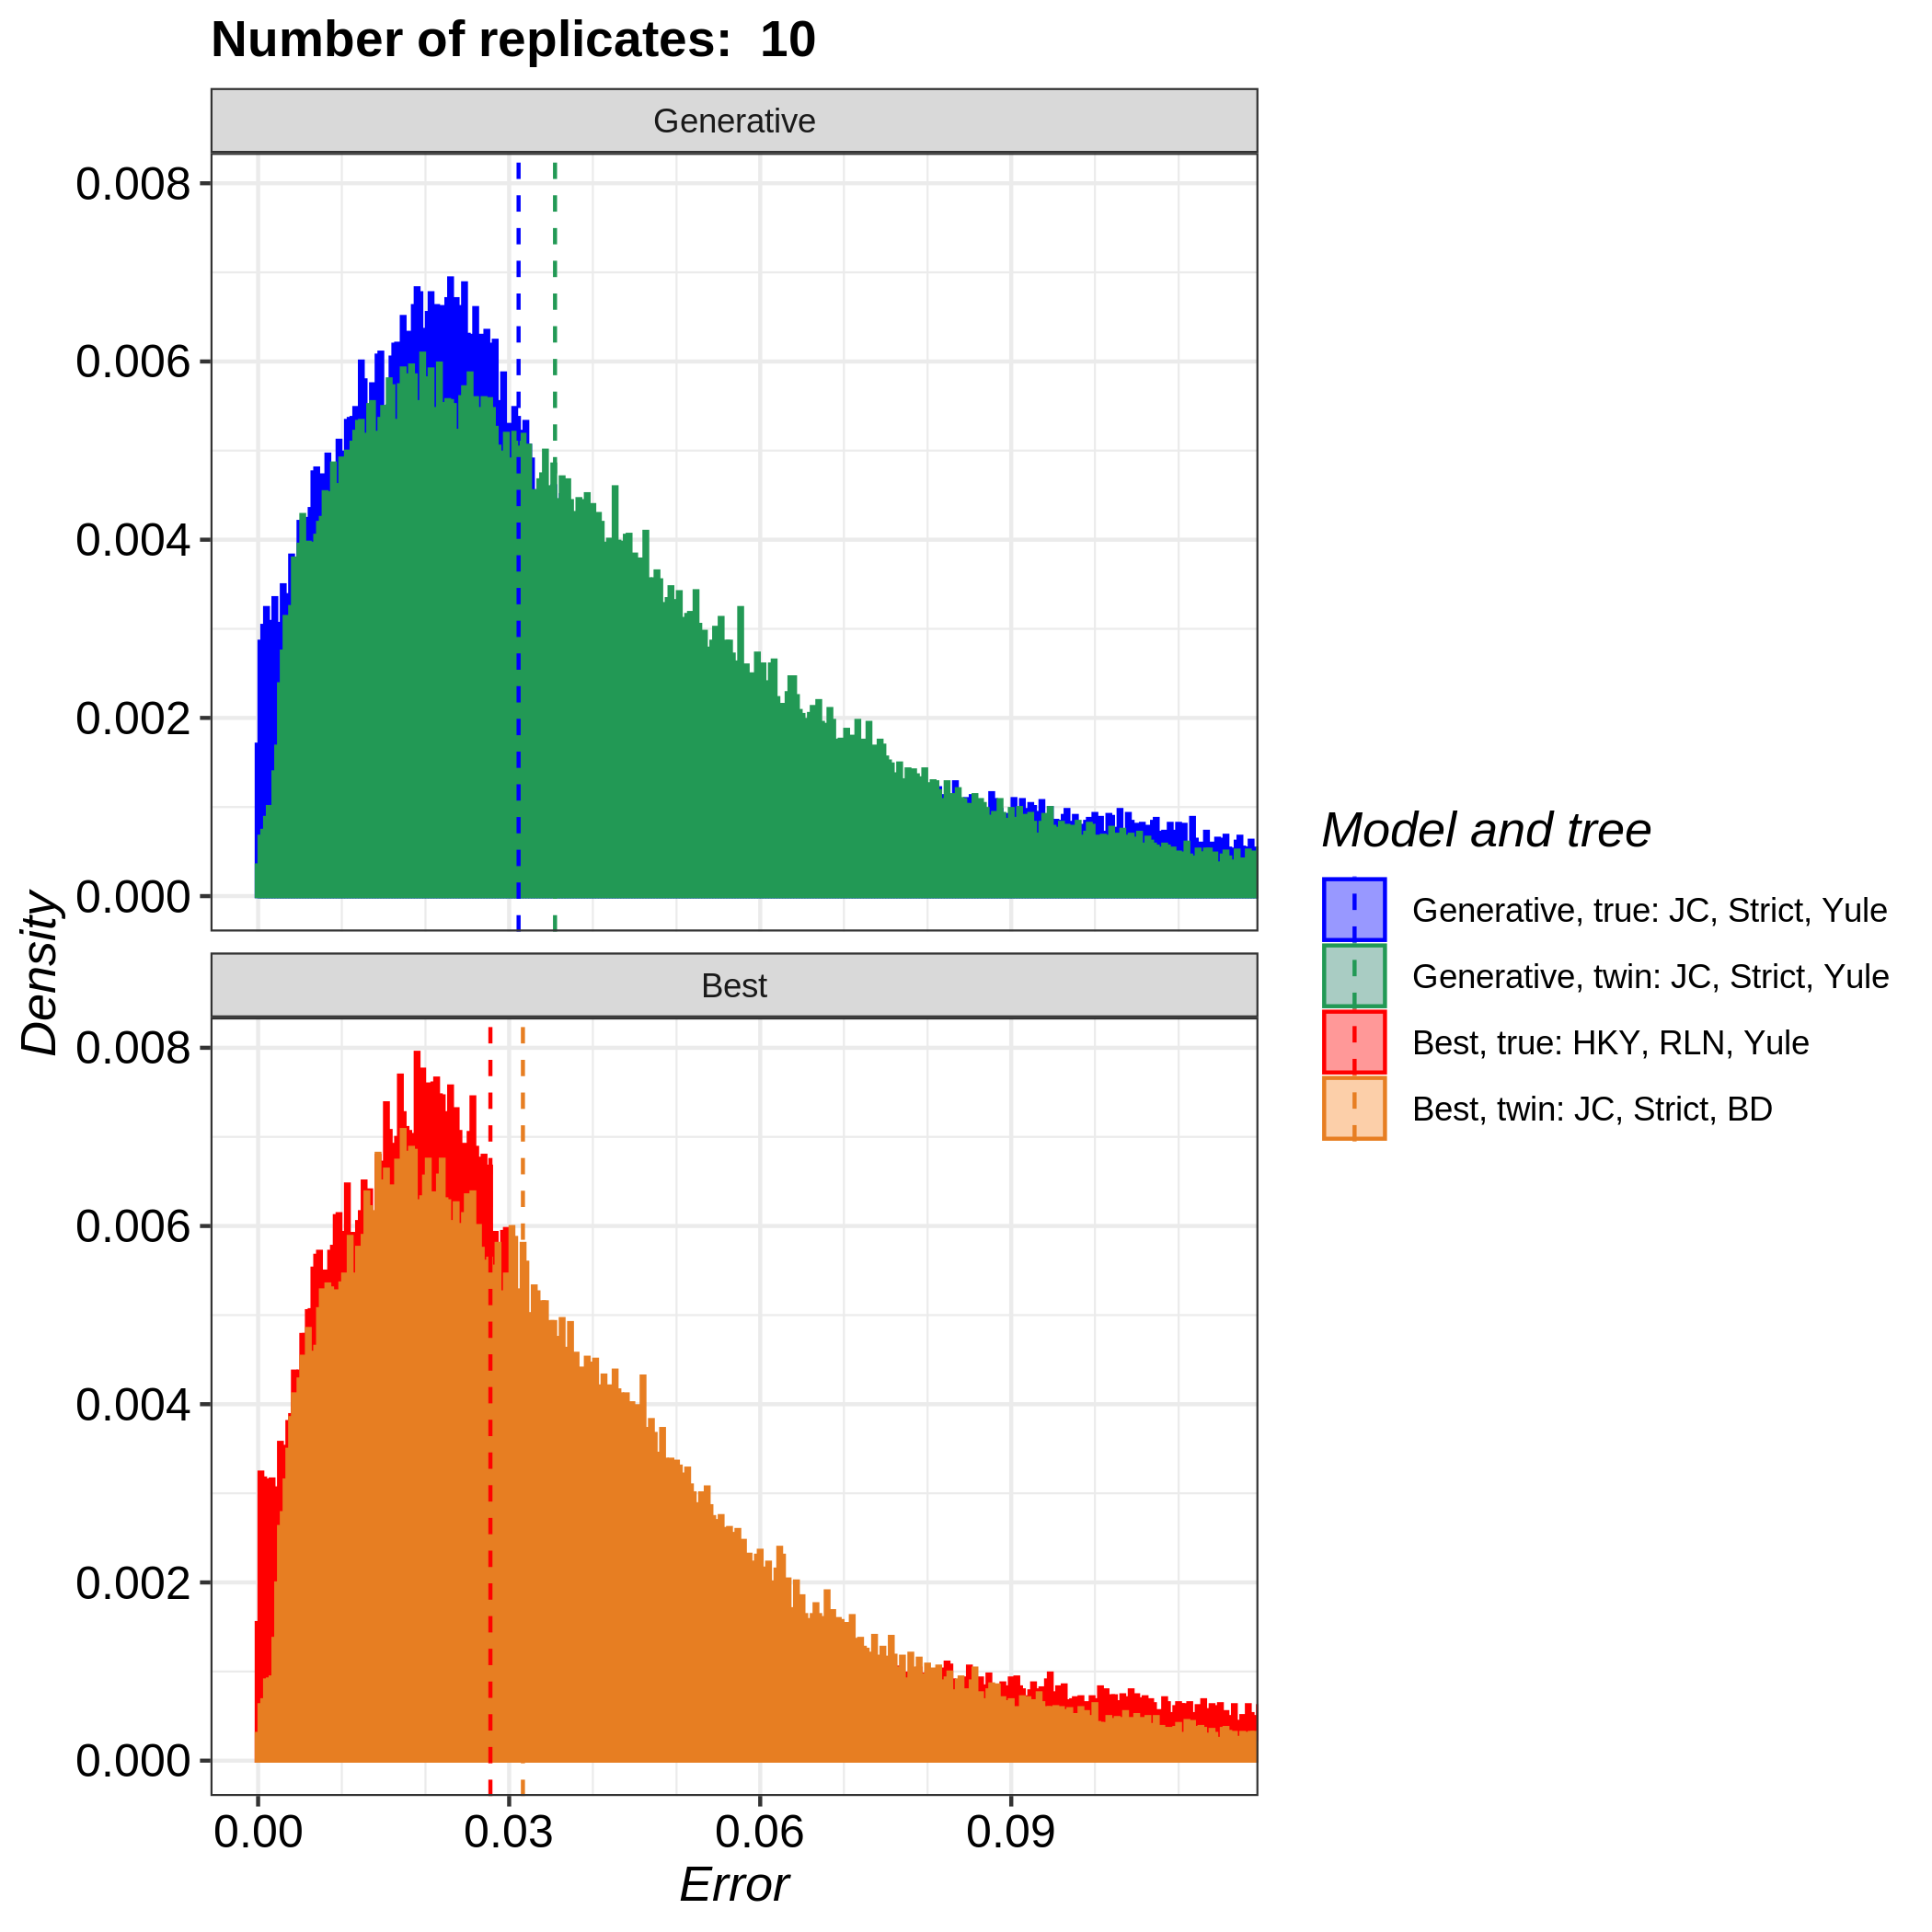
\includegraphics[width=\textwidth]{pirouette_example_39/errors.png}
  \caption{Per-nucleotide mutation rate of 1.50 / crown age, 10 hours}
\end{figure}

\begin{figure}[H]
  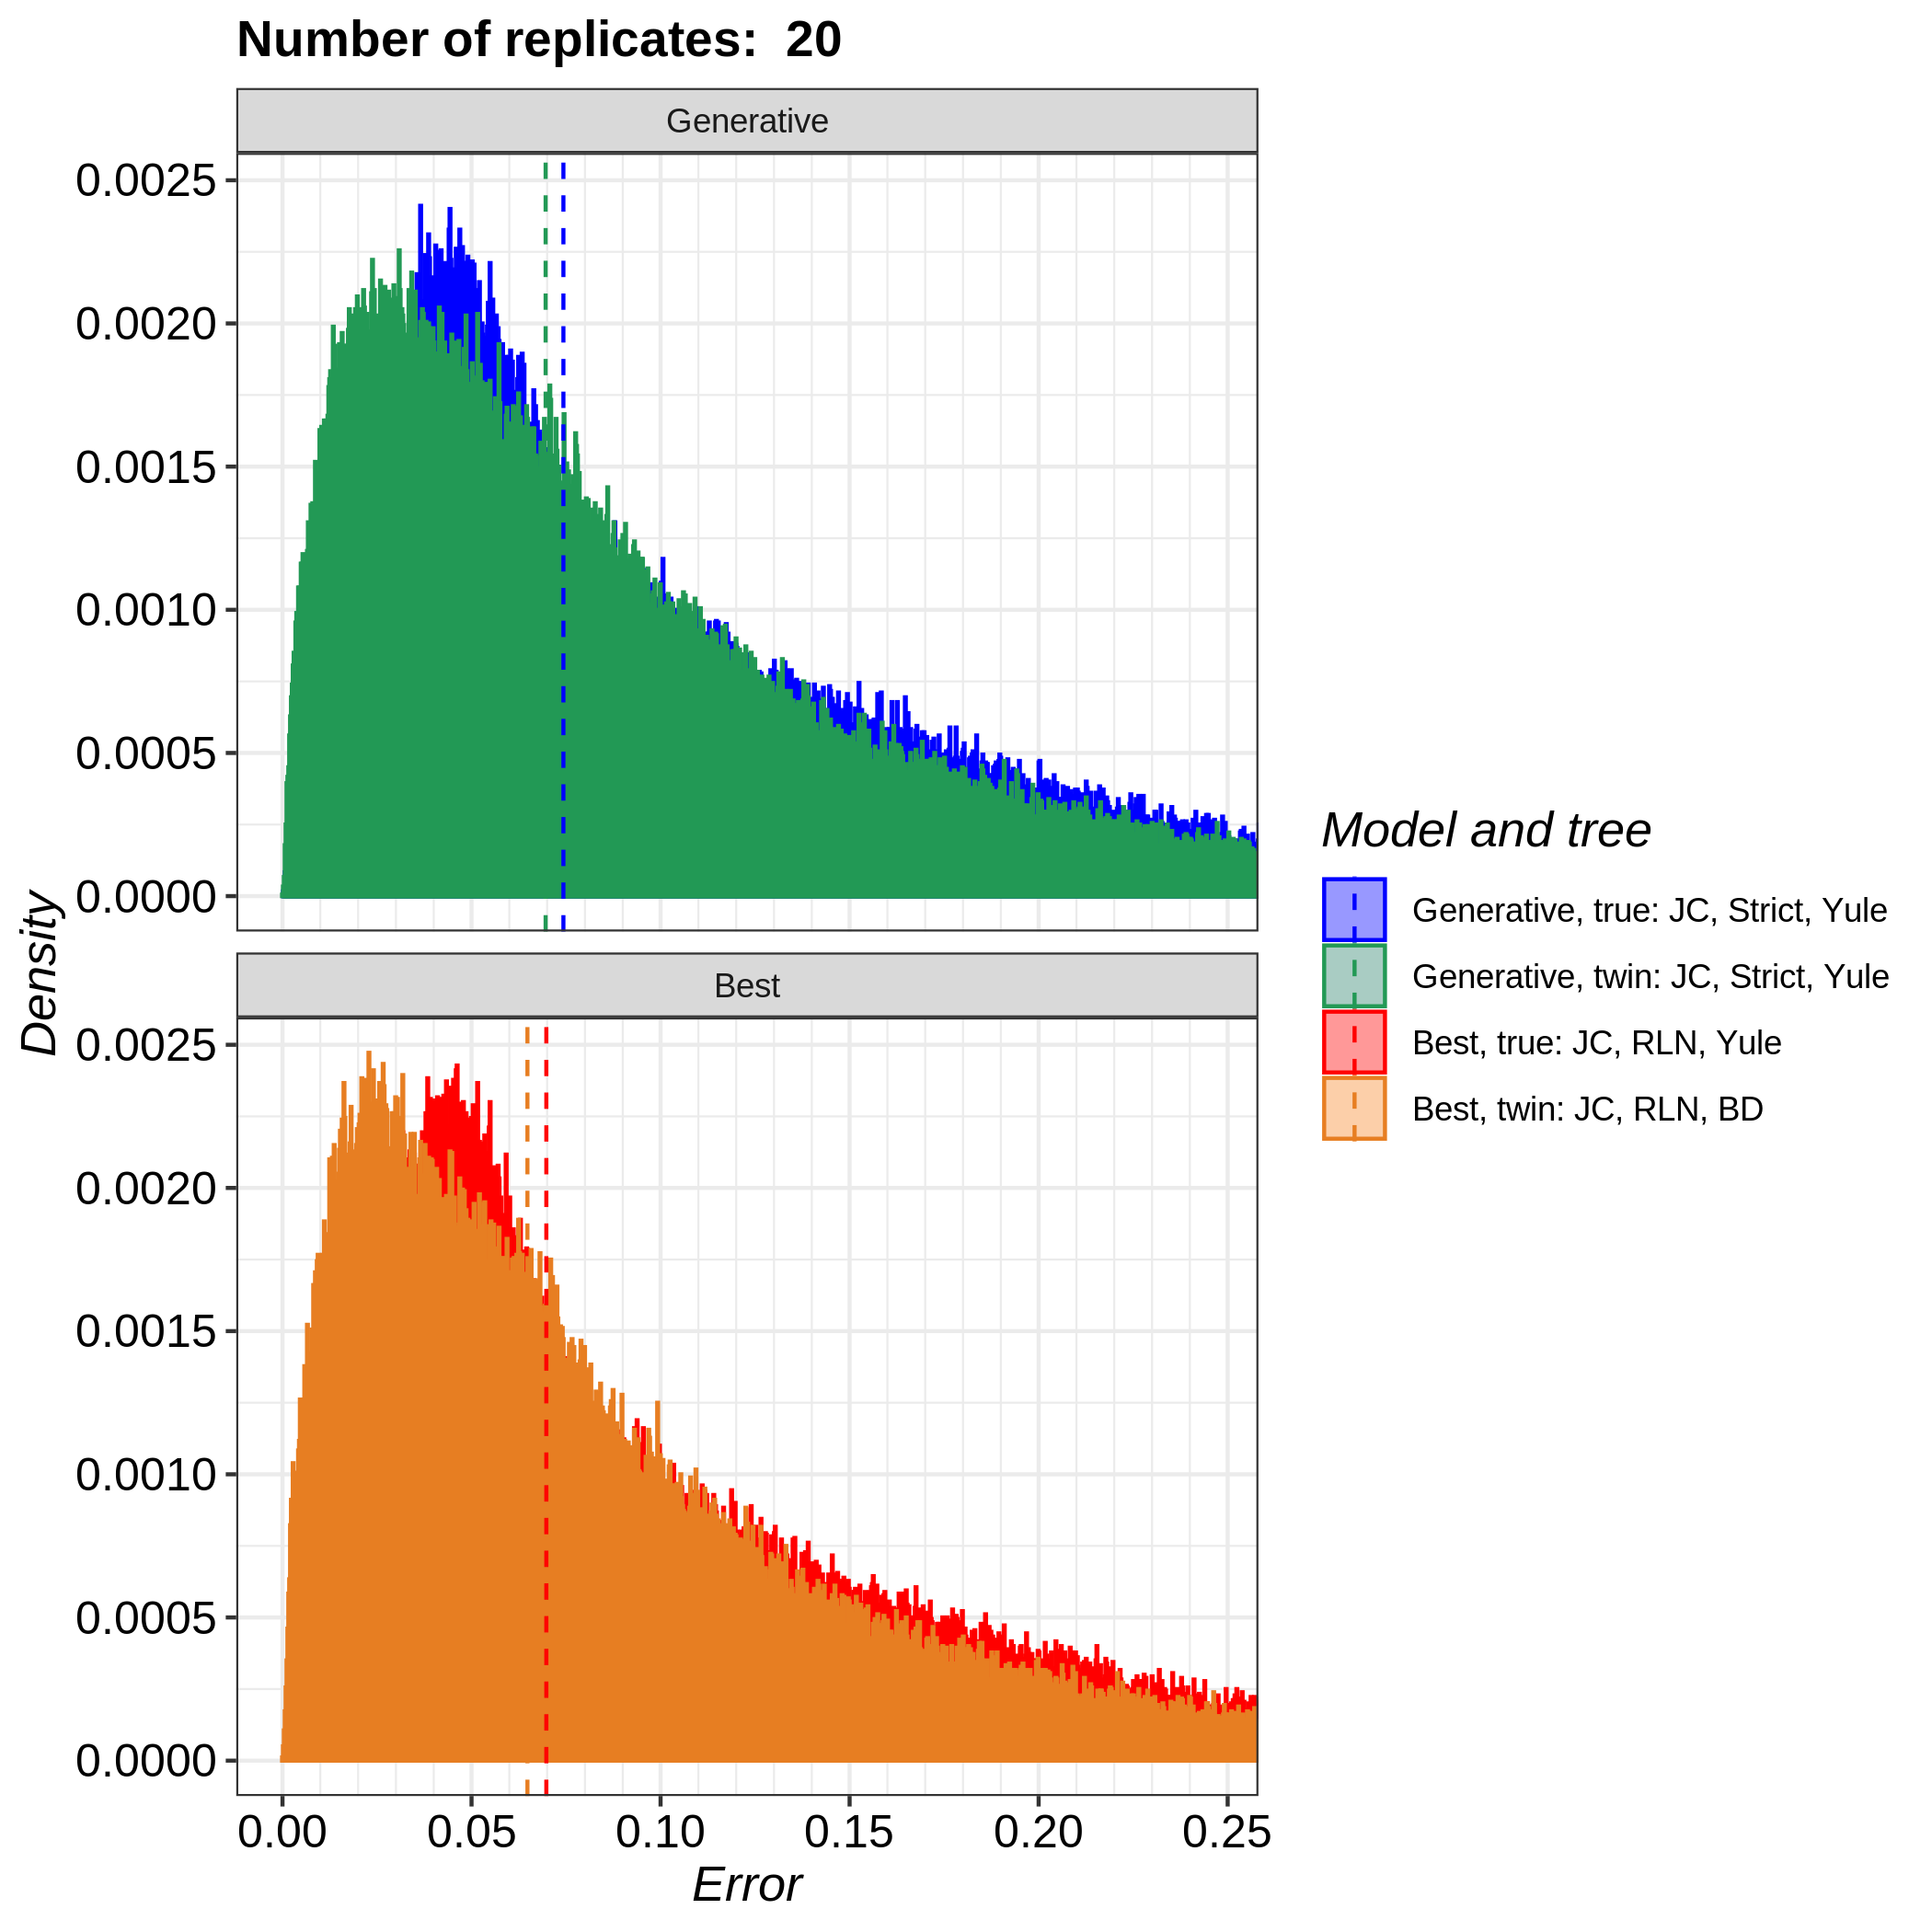
\includegraphics[width=\textwidth]{pirouette_example_40/errors.png}
  \caption{Per-nucleotide mutation rate of 2.0 / crown age, 19 hours}
\end{figure}

